\documentstyle[psfig,html]{article}

% use %sort -f -u manual.idx > manual.index for a primitive index

%%%%%%%%%%%%%%%%%%% No changes beyond this point %%%%%%%%%%%%%%%%%%%%%%%%%%%%%

\makeindex
%\psdraft
% Transforms the \indexentry generated by \makeindex in the concepts.idx
% file into a form understood by the theindex environment.
% See below on h	ow to produce an index.
\newcommand{\latextohtml}{ {\bf LaTeX}{2}{\tt{HTML}} }
\newcommand{\fn}{\tt}	% file names
\newcommand{\indexentry}[2]
   {\item #1 #2}

\setlength{\textwidth}{5.5in}
\addtolength{\oddsidemargin}{-1in}
\addtolength{\evensidemargin}{-1in}
\begin{document}
\sloppy
\title{The LaTeX2HTML Translator}
\author{Nikos Drakos,\\ Computer Based Learning Unit,\\ University of
Leeds.}
\date{\today}
\maketitle 

\centerline{This document accompanies LaTeX2HTML Version 95}

\begin{htmlonly}
A \htmladdnormallink{postscript
version}{http://cbl.leeds.ac.uk/nikos/tex2html/doc/manual.ps}
is available. \index{postscript version}

{\bf Warning:} The contents of this document are likely to change.
It is advisable not to use links to any pages other than the first
page (this page).
\end{htmlonly}

\begin{abstract} 
\latextohtml is a conversion tool that allows documents
written in LaTeX to become part of the WorldWide Web.
In addition, it offers an easy migration path towards
authoring complex hypermedia documents using
familiar word-processing concepts.

\latextohtml replicates the basic structure of a LaTeX document 
as a set of interconnected HTML files which can be explored using
automatically generated navigation panels. 
The cross-references, citations, footnotes, the table of contents and the lists
of figures and tables, are also translated into hypertext links. Formatting
information which has equivalent ``tags'' in HTML (lists, quotes, paragraph
breaks, type styles, etc.) is also converted appropriately. 
The remaining heavily formatted items
such as mathematical equations, pictures or tables are converted to images
which are placed automatically at the correct positions in the
final HTML document.

\latextohtml extends LaTeX by supporting arbitrary hypertext links 
and symbolic cross-references between evolving 
remote documents. It also allows the specification
of {\em conditional text} and the inclusion of raw HTML commands.
These hypermedia extensions to LaTeX are available as 
new commands and environments from with a LaTeX document.

This document presents the main features of \latextohtml, and
describes how to obtain, install, and use it.
\end{abstract}

\pagebreak
\tableofcontents
\listoffigures
\listoftables

\pagebreak

\section{Overview}
\index{overview}
This document describes the \latextohtml translator which:

\begin{itemize}
\item breaks up a document into one or more components as specified
by the user\footnote{The user can specify the {\em depth} at which 
the document should not be broken up any further.},
\item provides optional, customizable iconic navigation
panels on every page which contain links to other parts of the
document, or other documents,
\index{inlined equations}
\item hadles inlined equations ( \(\sum_{i=1}^{n} x_{i} =
\int_{0}^{1} f \)), handles equation alignment ($A_{B_{C+D}}$), 
right-justified numbered equations
(see equation \ref{eq:demo}), tables (see Table \ref{tab}), or
figures (see Figure \ref{fig:example}),
and {\em any arbitrary environment}\footnote{These are
passed to LaTeX and then converted to images which are either included
in the document or are made available through hypertext links.},

\item 
figures or tables can be arbitrarily scaled and shown either as
inlined images or ``thumbnail'' sketches
\item can produce output suitable for browsers that support inlined
images or character based browsers (as specified by the user),
\item handles definitions of new commands, environments, and theorems
even when these are defined in external style files\footnote{
This allows the definition of HTML macros in LaTeX  !},
\item handles footnotes\footnote{Like this!}, tables of contents, lists
of figures and tables, bibliographies, and can generate an
\index{index} index,
\item translates cross-references into hyperlinks and 
extends the LaTeX cross-referencing mechanism to work
not just within a document but {\em between documents} which may
reside in remote locations, \index{ISO-LATIN-1}
\item translates LaTeX accent and special character commands
(e.g. \. {A} \O \"o \pounds \copyright \P) to
the equivalent ISO-LATIN-1 character set where possible,
\item recognizes hypertext links (to multimedia resources or
arbitrary internet services such as sound/video/ftp/http/news) and
links which invoke arbitrary program scripts,
all expressed as LaTeX commands,
\item recognizes {\em conditional text}  which is intended only for
the hypertext version, or only for the paper (DVI) version,
\item can include raw HTML in a LaTeX document (e.g. in order to
specify interactive forms),
\item can deal sensibly at least with the {\em Common LaTeX  commands}
summarized at the back of the LaTeX  blue book \cite{lamp:latex},
\item will try and translate any document with embedded LaTeX commands 
irrespective of whether it is complete or syntactically legal.
\end{itemize}

A selection of documents illustrating the different contexts in 
which \latextohtml has been used is available at \\
\htmladdnormallink{http://cbl.leeds.ac.uk/nikos/tex2html/doc/latex2html/latex2html.html}{http://cbl.leeds.ac.uk/nikos/tex2html/doc/latex2html/latex2html.html}.

\section{User Manual}
\index{man page} \label{sec:man}

To use \latextohtml simply type {\fn latex2html $<$file$>$.tex}. This 
will create a new directory called {\tt file} which will contain 
the generated HTML files, some log files and possibly some images.
To view the result use an HTML viewer such as \htmladdnormallink{NCSA 
Mosaic}{http://www.ncsa.uiuc.edu/SDG/Software/Mosaic/Docs/help-about.html}
on the main HTML file which is {\fn file/file.html}. This file will
contain navigation links to the other parts of the generated document.

It is possible to customize the output from \latextohtml using a number
of \hyperref{command line options}{command line options (see Section
}{)}{options}
with which you can specify how to break up the document, where to put 
the generated files, what the title is, what the signature at the end
of each page is, what to put in the navigation panel, what kind of
extra information to include about the document, whether to retain
the original LaTeX section numbering scheme, etc.

Also, the \latextohtml script includes a short manual which can be 
viewed by saying 
{\tt \verb|%nroff -man latex2html| }.

\subsection{Command Line Options}
\index{options}\label{options}
The command line options described below can be used to change the
default behavior of \latextohtml. Alternatively, the corresponding 
environment variables
in the initialization file {\fn .latex2html-init} may be changed, in
order to achieve the same result.

\begin{description}
\item [-split num]
Stop splitting sections into separate files at this depth.
A value of 0 will put the document into a 
single HTML
file. The default is 8.
\item [-link num]
Stop revealing child nodes at each node at this depth. 
(A node is a part/chapter/section/subsection/subsubsection etc.).
A value of 0 will show no links to child nodes, a value of 1 
will show only the immediate descendents, etc. A value
at least as big as that of the {\tt -split}
option will produce a table of contents for
the tree structure, rooted at each given node. The default is 4.
\label{page:nolatex}
\item [-nolatex ]
Disable the mechanism for passing unknown environments to LaTeX   for processing.
This can be thought of as ``draft mode'' which allows  faster translation of the 
basic document structure and text, without fancy figures, equations or
tables. 

{\bf This option has been superceded by the {\tt -no\_images} option
(see below)}.
\item [-external$\_$images]
Instead of including any generated images inside the document, leave them
outside the document and provide hypertext links to them.
\label{asciimode} 
\item [-ascii$\_$mode]
Use only ascii characters and do not include any images in the final output.
In ascii mode the output of the translator can be used on
character based browsers which do not support inlined images (the $<$IMG$>$ tag).
\item [-t top-page-title]
Name the document using this title.
\item [-dir output-directory]
Redirect the output to this directory. 
\item [-no\_subdir]
Place the generated HTML files  in the 
current directory. The default behaviour is to create (or reuse)
another file directory.
\item [-ps\_images]
Use links to external postscript images rather than inlined GIF images.
\item [-address author-address]
Sign each page with this address. \label{navoptions} 
\item [-no$\_$navigation]
Disable the mechanism for putting navigation links in 
each page.
\item [-top$\_$navigation]
Put navigation links 
at the top of each page.    
\item [-bottom$\_$navigation]
Put navigation links 
at the bottom of each page AS WELL as the top.
\item [-auto$\_$navigation]
Put navigation links
at the top of each page. If the page exceeds \verb|$WORDS_IN_PAGE| number of words
(the default is 450) then put one at the bottom of the page as well.
\item [-index$\_$in$\_$navigation]
Put a link to the index page in the navigation panel if there is an index.
\item [-contents$\_$in$\_$navigation]
Put a link to the table of contents in the navigation panel if there is a 
table of contents.
\item [-next$\_$page$\_$in$\_$$\_$navigation]
Put a link to the next logical page in the navigation panel.
\item [-previous$\_$page$\_$in$\_$$\_$navigation]
Put a link to the previous logical page in the navigation panel.
\item [-info string]
Generate a new section {\em About this document ...} containing information
about the document being translated. The default is to generate such a section 
with information on the original document, the date, the user and the
translator.
An empty string (or the value 0) disables the creation of this extra
section. If a non-empty string is given, it will be placed in the contents of the 
{\em About this document ...} section instead of the default information.
\item [-dont$\_$include file(s)]
Do not include the specified file(s). Such files are usually style files which
may contain raw TeX commands that LaTeX or the translator cannot handle. 
\item [-reuse]
Reuse images generated during previous translations where appropriate.
This also disables the initial interactive session during which the user is
asked whether to reuse the old directory, delete its contents or quit.
Images which depend on context (e.g. numbered tables or equations)
cannot be reused and are always re-generated.
\item [-no\_reuse]
Do {\bf not} reuse images generated during previous translations.
(This will enable the initial interactive session during which the user is
asked whether to reuse the old directory, delete its contents or quit)
\item [-init$\_$file file]
Load the specified file. This Perl file will be loaded after loading 
\$HOME/.latex2html-init (if one exists). It can be used to change the 
default options.
\item [ -no\_images]
Do not attempt to produce any inlined images. 
The missing images can be generated "off-line" by restarting \latextohtml
with the option {\tt -images\_only}.
\item [ -images\_only]
Try and convert any inlined images that were left over from previous
runs of \latextohtml. 
\item [ -show$\_$section$\_$numbers]
Show section numbers. By default the section numbers are not shown 
in order to encourage the 
use of particular sections as standalone documents. 
In order to be shown, section titles must be unique and must not
contain inlined graphics.
\item [-h]
Print out the list of options.
\end{description}

\subsection{Extending the Translator}
\label{sec:extend}
As the translator covers only partially the set of LaTeX commands
and
because new LaTeX commands can be defined arbitrarily using low level 
TeX commands, the translator should be flexible enough to allow end
users
to specify how they want particular commands to be translated. 

\subsubsection{Adding Support for Specific Style Files}
\label{sec:sty}
\latextohtml provides a mechanism where code to translate specific
style files is automatically loaded if such code is available.
When the use of a style
file such as {\fn german.sty} is detected in a LaTeX source
document,
the translator looks for a file {\fn LATEX2HTMLDIR/styles/german.perl}.
If one is found, then it will be loaded into the main script. 

This mechanism will help to keep the core script smaller as well as make
it easier for others to contribute and share solutions on  
how to translate specific style files. The current distribution includes the files
{\fn german.perl}, {\fn french.perl}, {\fn html.perl} and {\fn makeidx.perl}.

The problem however, is that writing such extensions requires an understanding 
of Perl and of the way \latextohtml is organized. More user-friendly 
interfaces will be  investigated.

At the moment a rudimentary mechanism is provided so that 
a user can ask for particular commands and their arguments either to be
ignored or passed on to LaTeX for processing (the default behavior
for unrecognized commands is for their arguments to remain in the HTML
text).
Commands that are passed on to LaTeX are converted to images which
are either ``inlined'' in the main document or become accessible via
hypertext links.
Simple extensions using the commands above may be included in the 
{\fn LATEX2HTMLDIR/latextohtml.config} file or in each personal 
{\fn HOME/.latex2html-init} initialization file.

\subsubsection{Asking the Translator to Ignore Commands}
Commands that should be ignored may be specified in the {\fn
.latex2html-init}
file as input to the {\tt {\verb|ignore_commands|}} subroutine. 
Each command which is to be ignored should be on a separate line 
followed by compulsory or optional argument markers separated by 
{\verb|#|}'s e.g.\footnote{It is possible to add arbitrary Perl code
between any of the argument markers which will be executed when 
the command is processed. For this however a basic understanding of
how the translator works and of course Perl is required.}:
\begin{verbatim}
<cmd_name>#{}# []# {}# [] ...
\end{verbatim} 
\verb|{}|'s mark compulsory arguments and \verb|[]|'s optional ones.

Some commands may have arguments which should be left as
text even though the command should be ignored (e.g. {\tt mbox}, {\tt
center}, etc). In these cases the arguments should be left unspecified.

Here is an example of how this mechanism may be used:
\begin{verbatim}
&ignore_commands( <<_IGNORED_CMDS_);
documentstyle # [] # {}
linebreak# []
center
<add your commands here>
_IGNORED_CMDS_
\end{verbatim}
\subsubsection{Asking the Translator to Pass Commands to LaTeX}
\label{pass}
Commands that should be passed on to LaTeX for processing because
there is no direct translation to HTML may be specified in the {\fn
.latex2html-init}
file as input to the {\tt {\verb|process_commands_in_tex|}}
subroutine.
The format is the same as that for specifying commands to be ignored.
Here is an example:
\begin{verbatim}
&process_commands_in_tex (<<_RAW_ARG_CMDS_);
fbox # {}
framebox # [] # [] # {}
<add your commands here>
_RAW_ARG_CMDS_
\end{verbatim}
\section{Special Features}
\label{special} \index{hypertext extensions}
This section describes some special features of the translator which
can be considered as {\em hypertext extensions to \LaTeX}.
These are implemented as new LaTeX commands which have special 
meaning during the translation to HTML but are mostly ignored when
processed by \LaTeX.

\index{html.sty}
All the new commands used in the sections 
below are defined in the file \htmladdnormallink{{\fn html.sty}} 
{http://cbl.leeds.ac.uk/nikos/tex2html/doc/html.sty.txt} which is part of the 
distribution. {\em This file must be included in any 
LaTeX document using these features}\footnote{As an argument to the 
{\tt documentstyle} command or as an argument to the {\tt input}
command or by pasting the definitions of individual commands
directly into the text!}.

\subsection{Hyperlinks in LaTeX}
\label{sec:hyper} \index{hyperlinks} \index{htmladdnormallink} \index{htmladdimg}
Arbitrary hypertext references are available 
through the commands 
{\tt htmladdnormallink} and {\tt htmladdimg}).

These are defined as follows:
\begin{verbatim}
\htmladdnormallink{<text>}{<URL>}
\htmladdimg{<URL>}
\end{verbatim}
The first command expects some text as the first argument and a URL as
the second argument. When processed by LaTeX (i.e. in the {\tt dvi }
or {\tt ps} output files), the URL will have no effect.
But when processed by the 
translator, 
\htmladdnormallink{the URL will be used to provide
an active hypertext link}
{http://www.ncsa.uiuc.edu/demoweb/url-primer.html} (to another
file, picture, sound file, movie, etc) e.g.
\begin{verbatim}
\htmladdnormallink{<URL>}
	{http://www.ncsa.uiuc.edu/demoweb/url-primer.html}
\end{verbatim}

A similar command called {\tt htmladdnormallinkfoot} 
takes the same two arguments and has the same effect when generating
HTML as {\tt htmladdnormallink}. But when processed by LaTeX it shows
the 
URL as a footnote.

In a similar way, the argument of the {\tt htmladdimg} command 
should be a URL pointing
to an image. This URL is ignored in
the LaTeX hard copy output. 

\subsection{Cross-References Between Living Documents}
\label{external}
This section describes a mechanism for establishing cross-references
between two or more
documents via symbolic labels which are independent of
the physical realisation of these documents. 
The documents involved may reside in remote locations
and may be spread across one or more HTML files. 

The mechanism
is an extension of the simple {\tt label-ref} pairs which can be used only 
within a single document. A symbolic label defined with a 
{\tt label} command can be referred to using a {\tt ref} command.
When processed by LaTeX, each {\tt ref} command is replaced by the 
section number in which the corresponding {\tt label} occurred.
When processed by the translator, each {\tt ref} is replaced by 
a hypertext link to the place where the corresponding {\tt label}
occurred. The new commands detailed below show how it is possible to
refer to symbolic labels defined with {\tt label} in other external
documents.
Such references to external symbolic labels are then translated
into hyperlinks pointing to the external document.

\index{externallabels} \index{externalref} 
Cross-references between documents are established with the commands:
\begin{verbatim}
\externallabels{<URL to directory of external document>}
               {<external document labels.pl file>}

\externalref{<label in remote document>}
\end{verbatim}

\index{labels.pl} 
The first argument to {\tt externallabels} should be a URL to 
the directory containing the external document.  
The second argument
should be the full pathname to the {\tt labels.pl} file belonging
to the external document. The file {\tt labels.pl} associates symbolic
labels with physical files and is generated automatically for each 
translated document\footnote{Note that for {\em remote} external
documents
it is necessary to copy the {\tt labels.pl} file locally so that it
can be read when processing a local document that uses it.}.
The command {\tt externallabels} can be used once for each external
document in order to import the external labels into the current document.
The argument to {\tt externalref} may be any symbolic label defined 
in any of the external documents in the same
way that the {\tt ref} command refers to  labels defined internally.


After any modifications in an external document (sections added/deleted,
segmentation into different physical parts etc.) a new {\tt labels.pl}
will be generated. If the {\tt externallabels} command in another 
document contains the correct address
to the {\tt labels.pl} file then the cross-references will be
realigned
after running the local document through the translator. A warning is
given
if {\tt labels.pl} cannot be found.
\subsubsection{Example}
\label{crossrefs} 
To understand this mechanism better consider 
how you would maintain a link to this section  
(of the hypertext version of this document) from one of your documents
without using labels.
Sure enough you can get the
name of the physical file that this section is in. This however is very
likely to change and any links to it will become invalid. To update 
your link, the name of the new file must be found and your link changed 
by hand. Also there is no general updating mechanism so the only way to
find
out if your document is pointing to the right place is by actually
following the link and then doing a manual update\footnote{
Link validation can be done automatically but the updating must be
done
manually when filenames have changed (assuming no other symbolic label
mechanism is available).}.

Now consider how it could be done with symbolic labels. 
First you have to import the labels used in this document 
by copying the file 
\htmladdnormallink{labels.pl}
{http://cbl.leeds.ac.uk/nikos/tex2html/doc/manual/labels.pl},
saving it say
in {\tt /tmp/labels.pl},
and then adding anywhere in your document:
\begin{verbatim}
\externallabels{http://cbl.leeds.ac.uk/nikos/tex2html/doc/manual}
               {/tmp/labels.pl}
\end{verbatim}
After that you can use the label {\tt crossrefs} defined at the beginning of this 
section\footnote{You either have to guess the role of each label by
looking at the {\tt labels.pl} file or by asking the author!} as follows:
\begin{verbatim}
\externalref{crossref}
\end{verbatim}
This will be translated into the appropriate hyperlink to this page.
If there are any changes in this document and you would like to
bring your document upto date you have to copy 
\htmladdnormallink{labels.pl}
{http://cbl.leeds.ac.uk/nikos/tex2html/doc/manual/labels.pl} again
and rerun the translator on your document. Of course if I move the 
directory containing the HTML files for this document somewhere else 
then you would have to make a change in the argument of the 
{\tt externallabels} command to reflect this. 

It is obvious that some level of collaboration is required between
authors
trying to maintain cross-references between different documents. 
Using symbolic labels makes this a lot easier (especially for documents
written by the same author).

\subsection{Including Arbitrary HTML Markup}
\index{HTML+} 
Raw HTML or HTML+ tags and text may be included using the environment {\tt
rawhtml}. This can be used to take advantage
of new HTML+ facilities as soon as they become available.
\index{electronic forms} A particularly
good use of this feature is in the creation of interactive
\htmladdnormallink{electronic forms}{http://south.ncsa.uiuc.edu/forms.html}
from within a LaTeX document. When producing the paper (DVI) version
of a document the {\tt rawhtml} environment is ignored.

Here is an example: \index{rawhtml}
\begin{small}
\begin{verbatim}
\begin{rawhtml}
<HR>
<FORM ACTION="http://cbl.leeds.ac.uk/nikos/doc/error.html">
<OL>
<LI> <INPUT TYPE="checkbox" NAME="wp" VALUE="word"> Word for
Windows.
<LI> <INPUT TYPE="checkbox" NAME="wp" VALUE="wp"> Word Perfect.
\end{verbatim}
\begin{verbatim}
<LI> <INPUT TYPE="checkbox" NAME="wp" VALUE="latex"> LaTeX.
<LI> Plain Text Editors (Please Specify): <INPUT TYPE="text" NAME="other_ed">
</OL>
So, what do think (comments please): <BR>
<INPUT TYPE="text" SIZE=45,4 NAME="other_wp">

<INPUT TYPE="submit" VALUE="submit this form but don't expect much!">
</FORM>
<HR>
\end{rawhtml}
\end{verbatim}
\end{small}
\begin{rawhtml}
The result is shown below. 
<HR>
<FORM ACTION="http://cbl.leeds.ac.uk/nikos/doc/error.html">
<OL>
<LI> <INPUT TYPE="checkbox" NAME="wp" VALUE="word"> Word for
Windows.
<LI> <INPUT TYPE="checkbox" NAME="wp" VALUE="wp"> Word Perfect.
<LI> <INPUT TYPE="checkbox" NAME="wp" VALUE="latex"> LaTeX.
<LI> Plain Text Editors (Please Specify): <INPUT TYPE="text" NAME="other_ed">
</OL>
So, what do think (comments please): <BR>
<INPUT TYPE="text" SIZE=45,4 NAME="other_wp">

<INPUT TYPE="submit" VALUE="submit this form but don't expect much!">
</FORM>
<HR>
\end{rawhtml}

\begin{latexonly}
The result is shown below:
\begin{figure}[tbh]
    \begin{center}
    \framebox{
    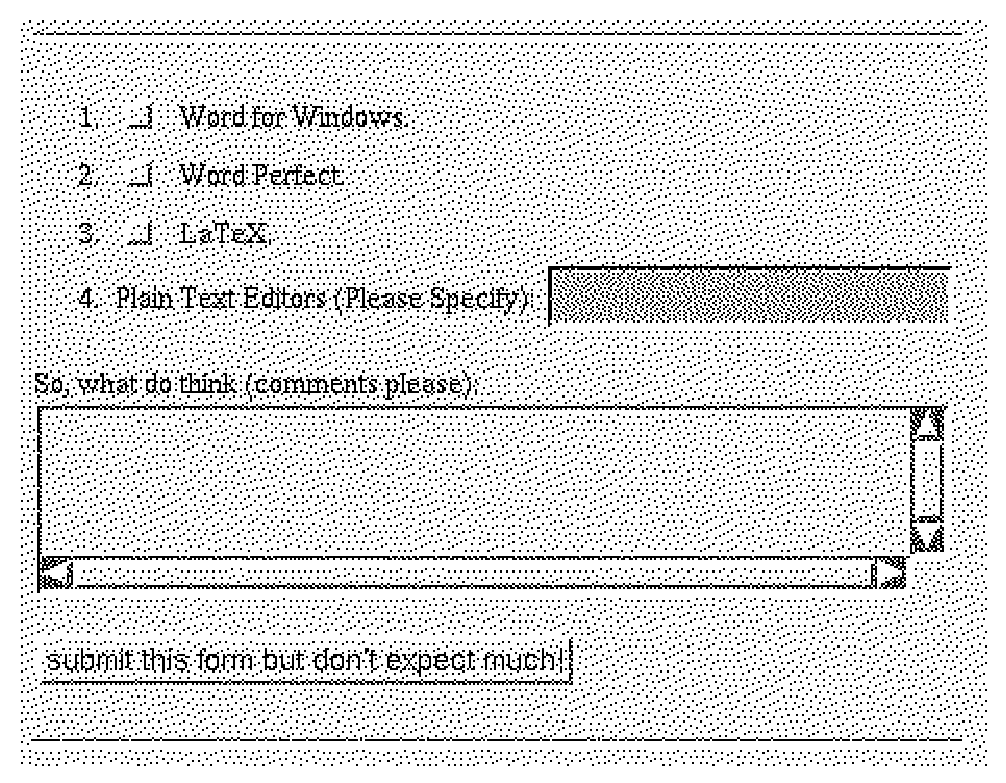
\psfig{file=eform.ps,width=4in}} \\
     Figure: An electronic form. Of course in the online version of this
document the form above would be active.
    \end{center}
\end{figure}
\end{latexonly}

{\bf Warning:} Avoid using LaTeX commands involving counters (e.g.
numbered figures or equations) in conditional text because this may 
disrupt the values of the counters in the electronic version.

% The argument here used to have a \label in its argument which caused
% the ``Contents'' page entry not to be hyperized.
\subsection{Conditional Text}
\label{sec:latexonly}
\index{latexonly} \index{htmlonly}
Conditional text can be specified using the environments {\tt latexonly} and {\tt
htmlonly}. These allow writing parts of a document which are intended
only for electronic delivery or only for paper-based delivery. 

This would be useful for example in adding a long description of a
multimedia resource in the paper version of a document. Such a
description would be redundant in the electronic version, as the user
can have direct access to this resource. 

Here is an example of the use of the {\tt latexonly} environment:

\begin{verbatim}
\begin{latexonly}
\begin{figure}
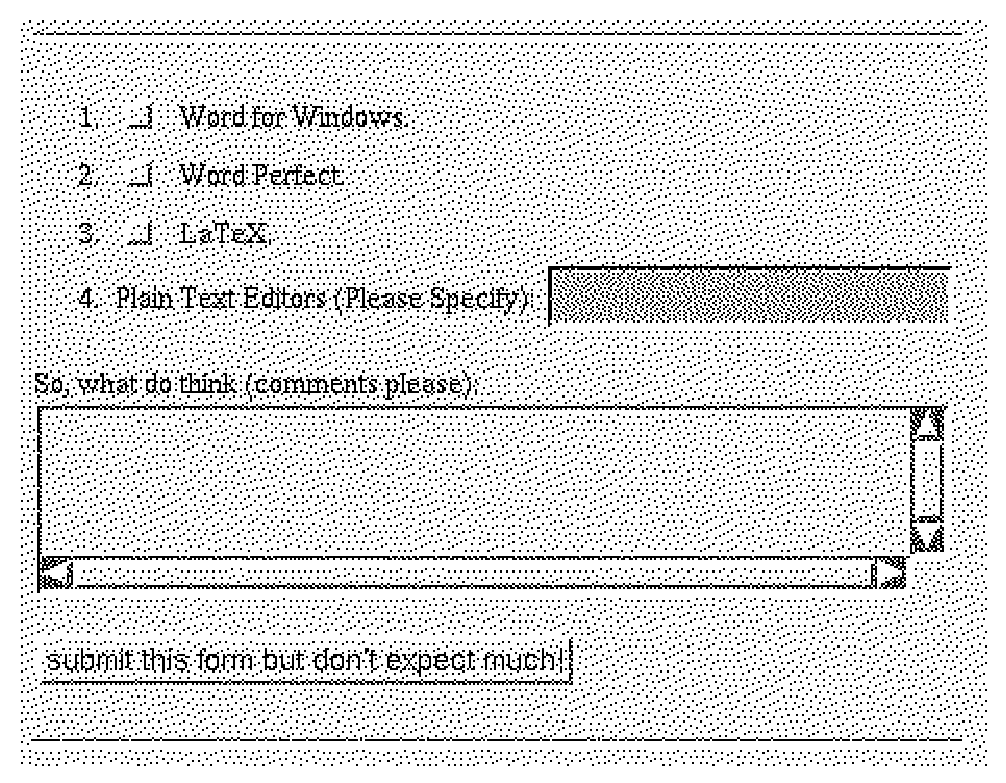
\psfig{file=eform.ps,width=4in}
\caption{An electronic form. Of course in the online version 
of this document the form above would be active!}
\end{figure}
\end{latexonly}
\end{verbatim} 

\subsection{Cross References Shown as ``Hyperized'' Text}

\index{cross-references}
In printed documents cross-references are shown through a {\em numerical
or symbolic indirection} e.g. ``see Figure 1'' (numeric indirection), or
``see section ``Changes'' (symbolic indirection).  \latextohtml can
mirror this mechanism using the same numeric or symbolic references,
or when these are
not appropriate by using iconic references.

In a hypertext document however, cross-references can be shown 
without any indirection just by highlighting a relevant piece of
text. This can make a document more readable as it removes unnecessary
information. 

A single new LaTeX command {\tt hyperref} can be used for
specifying how a cross-reference should appear both in the printed
document and in the hypertext version.

Assuming that the label \verb|sec:cond| is defined somewhere
in a document the command {\tt hyperref} which takes 4 arguments
can be used in the same document as follows:

\index{hyperref} \index{conditional text}
\begin{verbatim}
{\em Is the concept of
\hyperref
% This will be highlighted in the hypertext version
{conditional text}			% argument #1
% This will be shown in the printed version 
% followed by a numeric reference ...      
{conditional text (see Section }  	% argument #2
% ... followed by this text
{ for more information)} 		% argument #3
% This the common label 
{sec:cond}				% argument #4
a good idea? }
\end{verbatim}

Here is how it will be shown: \\
{Is the concept of
\hyperref
% This will be highlighted in the hypertext version
{conditional text}
% This will be shown in the printed version  
% followed by a numeric reference ...      
{conditional text (see Section }  
% ... followed by this text
{ for more information)} 
% This the common label 
{sec:cond}
a good idea? }

\begin{htmlonly}
In the printed version what would appear is: \\
{ Is the concept of conditional text (see Section XXX for more information) a good idea? }
\end{htmlonly}

\begin{latexonly}
In the hypertext version what would appear is:\\
{ Is the concept of \underline{conditional text} a good idea?} \\
Of course \underline{conditional text} would be an active hypertext link.
\end{latexonly}


Another command also defined in {\fn html.sty} is {\tt htmlref} 
which has the same effect as {\tt hyperref} during the conversion to
HTML.
It takes two arguments, some text and a label. In the HTML version the
text will be ``hyperized'' pointing to the label. In the paper version
the text will be shown as it is and the label will be ignored eg

\begin{small}
\begin{verbatim}
With {\tt htmlref} \htmlref{it's easy to make links}{fig:example}.
\end{verbatim}
\end{small}

\begin{htmlonly}
In the HTML version it will be shown as: \\
With {\tt htmlref} \htmlref{it's easy to make links}{fig:example}.
\end{htmlonly}
\begin{latexonly}
In the HTML version it will be shown as: \\
With {\tt htmlref} \underline{it's easy to make links}.
\end{latexonly}


\subsection{Customizing the Navigation Panel}
\index{navigation panel} \label{sec:navpanel}
The navigation panel is the strip containing ``buttons'' and text
that appears at the top
and perhaps at the bottom of each generated page and provides
hypertext
links to other sections of a document. Some of the
options and variables that control whether and where it should appear 
\hyperref{have already been mentioned}{have already been mentioned in 
Section }{}{navoptions}. 


A simple mechanism for appending customized buttons to the navigation
panel is provided by the command {\tt htmladdtonavigation}. This takes
one
argument which \latextohtml appends to the navigation panel. For
example,
\begin{verbatim}
\htmladdtonavigation
   {\htmladdnormallink
      {\htmladdimg{http://server/mybutton.gif}}
      {http://server/link}}
\end{verbatim}
will add an active button {\tt mybutton.gif} pointing to the specified location.


Apart from these facilities it is
also 
possible to specify completely what appears in the navigation panel 
and in what order. As each section is processed, \latextohtml
assigns relevant information to a number of global variables.
These variables are used by the subroutine {\fn navigation$\_$panel}
where the navigation panel is constructed as a string consisting of
these variables and some formatting information. 

This subroutine
can be redefined in a system or a user configuration file ({\fn
LATEX2HTMLDIR/latex2html.config} and {\fn HOME/.latex2html-init} 
respectively). {\em Any combination of text, HTML tags, 
and the variables mentioned below is acceptable}. 

The control panel variables are:

{\bf Iconic links (buttons)}
\begin{itemize}
\item PREVIOUS - points to the previous section 
\item UP  - points up to the "parent" section
\item NEXT - points to the next section
\item NEXT$\_$GROUP - points to the next "group" section
\item PREVIOUS$\_$GROUP - points to the previous "group" section
\item CONTENTS - points to the contents page if there is one
\item INDEX - points to the index page if there is one
\end{itemize}

{\bf Textual links (section titles)}
\begin{itemize}
\item PREVIOUS$\_$TITLE - points to the previous section
\item UP$\_$TITLE  - points up to the "parent" section
\item NEXT$\_$TITLE - points to the next section
\item NEXT$\_$GROUP$\_$TITLE - points to the next "group" section
\item PREVIOUS$\_$GROUP$\_$TITLE - points to the previous "group" section
\end{itemize}

If the corresponding section exists each iconic button will contain an
active link to that section. If the corresponding section does
not exist, the button will be inactive. If the section corresponding
to a textual link does not exist then the link will be empty.

The number of words that appears in each textual link
is controlled by the variable {\fn WORDS$\_$IN$\_$NAVIGATION$\_$PANEL$\_$TITLES}
which may also be changed in the configuration files.

Below is an example of a navigation panel 
(the ``.'' is the Perl string concatenation operator and ``\#''
signifies
a comment).

\begin{small}
\begin{verbatim}
sub navigation_panel {

    #  Start with a horizontal rule (3-d dividing line)
    "<HR> ".			
    
    # Now add few buttons with a space between them
    "$NEXT $UP $PREVIOUS $CONTENTS $INDEX $CUSTOM_BUTTONS" .
	    
    "<BR>\n" .		# Line break
	
    # If ``next'' section exists, add its title to the navigation panel
    ($NEXT_TITLE ? "<B> Next:</B> $NEXT_TITLE\n" : undef) . 
    
\end{verbatim}
\begin{verbatim}
    # Similarly with the ``up'' title ...
    ($UP_TITLE ? "<B>Up:</B> $UP_TITLE\n" : undef) . 
 
    # ... and the ``previous'' title
    ($PREVIOUS_TITLE ? "<B> Previous:</B> $PREVIOUS_TITLE\n" : undef) .
   
    #  Horizontal rule (3-d dividing line) and new paragraph  
    "<HR> <P>\n"		
}
\end{verbatim}
\end{small}

\subsection{Indicating Differences Between Document Versions} 

\latextohtml supports the {\fn changebar.sty} package by David B. Johnson 
(dbj@titan.rice.edu), for 
inserting ``change bars'' in a document in order to indicate 
differences from previous versions. This is a very primitive form of 
version control and there is much scope for improvement.


\subsection{Hypertext Links in Bibliographic References (Citations)}
If a report or a book that is cited (using the {\tt cite}) 
command is available (or there is information about it) on WorldWide
Web then it is possible to add the appropriate hypertext links
in your bibliographic database (the {\fn .bib}) file. 

Here is an example of a bibliographic entry for the original
LaTeX\cite{lamp:latex} book:

\begin{small}
\begin{verbatim}
@book{lamp:latex,
title = "LATEX User's Guide \& Reference Manual",
year = 1986 ,
author = "Leslie Lamport",
Publisher = "Addison-Wesley Publishing Company, Inc.",
note = "Online information on TeX and LaTeX is available at
\htmladdnormallink{http://curia.ucc.ie/info/TeX/menu.html}
{http://curia.ucc.ie/info/TeX/menu.html} and
\htmladdnormallink{http://es-sun2.fernuni-hagen.de/info2html?(latex.info)Top}
{http://es-sun2.fernuni-hagen.de/info2html?(latex.info)Top}"}
\end{verbatim}
\end{small}
No other
modifications are required for this to work - LaTeX and BibTeX 
should work as normal.

For those who use the Harvard style for references
\htmladdnormallinkfoot{there exists a special conversion
add-on package}{http://www.arch.su.edu.au/\~{}peterw/latex/harvard/}.

\subsection{Internationalization}
A special variable {\tt LANGUAGE\_TITLES} 
in the initialization or configuration files determines the language 
in which some section titles will appear. For example setting it to 
\begin{verbatim}
$LANGUAGE_TITLES = ``french'';
\end{verbatim}
will cause LaTeX2HTML to produce ``Table des mati\`{e}res'' instead of
``Table of Contents''.

The only languages currently supported are ``french'' and ``english''
but it is trivial to add support for another language in the
file {\fn latex2html.config}. As a guide here is the entry for 
the French titles:
\begin{verbatim}
sub french_titles {
 $toc_title = "Table des mati\\`eres";	
 $lof_title = "Liste des figures";
 $lot_title = "Liste des tableaux";
 $idx_title = "Index";
 $bib_title = "R\\'ef\\'erences";		
 $info_title = "\\`A propos de ce document..."; 
}
\end{verbatim}

In order to provide full support for another language you may also
want to replace the navigation buttons which come with \latextohtml 
(which are by default in
English)
with your own. As long as the new buttons have the same filenames as the
old ones there should not be a problem.

\subsection{Image Conversion}
\label{imgcon}

\latextohtml converts equations, special accents, external postscript
files, and LaTeX environments it cannot directly translate into 
inlined images. This section describes how it is possible to control
the final appearance of such images. For the purposes of the discussion below,

\begin{description}
\item[{\bf ``small images''}] will refer to equations, special accents and
any other image generating LaTeX commands, while 
\item[{\bf ``figures''}] will
apply  to any image generating LaTeX environments (eg figure, table,
minipage etc).
\end{description}

The size of all ``small images'' depends on a configuration variable
{\tt MATH\_SCALE\_FACTOR} which specifies how much to enlarge or 
reduce them in relation to their original size in the postscript 
version of the document. For example a scale factor of 0.5 will make all 
images half as big while a scale factor of 2 will make them twice as
big.
Larger scale factors result in longer processing times and larger 
intermediate image files. A scale factor will only be effective 
if it is greater than 0. 

The configuration variable {\tt FIGURE\_SCALE\_FACTOR} performs
a similar function for ``figures''. Both of these configuration 
variables are initially set to 1.6.

For finer control, several
parameters affecting the conversion of a single ``figure'' 
can be controlled
with the command {\tt htmlimage} which is defined in {\fn
html.sty}.
The one argument of {\tt htmlimage}
is a string of options separated by commas. The options are
\begin{verbatim}
scale = <scale factor>
external
thumbnail = <scale factor>
map = <image map URL>
\end{verbatim}

The {\tt scale} option allows control over the size of the final
image.

The {\tt external} option will cause the image not to be inlined 
(images are inlined by default). External images will be accessible
via a hypertext link. 

The {\tt thumbnail} option will cause a small inlined image to be 
placed in the caption. The size of the thumbnail depends on the
scale factor. The use of the {\tt thumbnail} option implies
the {\tt external} option. In order to be effective the command
{\tt htmlimage} and its options {\bf must be placed inside the
environment on which it will operate}.

The {\tt map} option will turn the inlined image into an 
\htmladdnormallink{active
image map}{http://wintermute.ncsa.uiuc.edu:8080/map-tutorial/image-maps.html}.

{\bf Example:}
The effect of the LaTeX commands below can be seen in the
\htmlref{thumbnail sketch of Figure}{fig:example} \ref{fig:example}.
\begin{small}
\begin{verbatim}
{\begin{figure}[tbh]
    \htmlimage{thumbnail=0.5}
    \centerline{
    \psfig{file=figure.ps,width=5in}}
    \caption{A sample figure showing part of a page generated by
\latextohtml containing a customized navigation panel (from the
\protect\htmladdnormallinkfoot{CSEP project}
{http://csep1.phy.ornl.gov/csep.html}).}
    \label{fig:example}
\end{figure}}
\end{verbatim}
\end{small}

The {\tt htmlimage} command is also often useful to cancel-out the
effect of the configuration variable {\tt FIGURE\_SCALE\_FACTOR}.
For example to avoid resizing a color screen snap despite 
the value of {\tt FIGURE\_SCALE\_FACTOR} it is possible to 
use {\tt htmlimage\{scale=0\}}.

\subsection{Figures, Tables and Arbitrary Environments}
\index{figures} These are here to show how the translator
handles figures, tables
and other environments. Compare the paper with the online version.

\index{tables}
\begin{table}[h]
\begin{center}
\begin{tabular}{||l|lr||}   \hline
gnats	&	gram	&	\$13.65  \\ \cline{2-3}
	&	each	&        .01	\\ \hline
gnu	& 	stuffed	&        92.50  
                \\  \cline{1-1} \cline{3-3}
emur	&		&	33.33   \\ \hline
armadillo	& frozen	&	8.99 \\ \hline
\end{tabular}
\end{center}
\caption{A sample table taken from \protect\cite{lamp:latex}}
\label{tab}
\end{table}

\index{numbered equations}
Here are some some automatically numbered right-justified equations
\begin{equation} 
\Phi_{l+1,m,n} = (\Phi+h\frac{\partial\Phi}{\partial x} +
\frac{1}{2}h^2\frac{\partial^2\Phi}{\partial x^2} +
\frac{1}{6}h^3\frac{\partial^3\Phi}{\partial x^3} + \ldots)_{l,m,n}
\end{equation}
with some gratuitously \'{a}cc\"{e}nted text in between them.
\begin{eqnarray}  \label{eq:demo}
\frac{\Phi_{l+1,m,n}-2\Phi_{l,m,n}+\Phi_{l-1,m,n}}{h^{2}} +
\frac{\Phi_{l,m+1,n}-2\Phi_{l,m,n}+\Phi_{l,m-1,n}}{h^{2}} + \nonumber \\
\frac{\Phi_{l,m,n+1}-2\Phi_{l,m,n}+\Phi_{l,m,n-1}}{h^{2}} = -I_{l,m,n}(v)
\end{eqnarray}

{\begin{figure}[tbh]
    \htmlimage{thumbnail=0.5}
    \centerline{
    \psfig{file=figure.ps,width=5in}}
    \caption{A sample figure showing part of a page generated by
\latextohtml containing a customized navigation panel (from the
\protect\htmladdnormallinkfoot{CSEP project}
{http://csep1.phy.ornl.gov/csep.html}).}
    \label{fig:example}
\end{figure}}

\section{Getting LaTeX2HTML}
\index{source code}
\begin{flushleft}
The \htmladdnormallink{source code can be obtained 
at http://cbl.leeds.ac.uk/nikos/tex2html/latex2html.tar.}
{http://cbl.leeds.ac.uk/nikos/tex2html/latex2html.tar}
or \htmladdnormallink{as a compressed archive at http://cbl.leeds.ac.uk/nikos/tex2html/latex2html.tar-gz}{http://cbl.leeds.ac.uk/nikos/tex2html/latex2html.tar-gz}
The source code is also available 
via anonymous FTP at 
\htmladdnormallink{ftp://ftp.tex.ac.uk/pub/archive/support/latex2html}{ftp://ftp.tex.ac.uk/pub/archive/support/latex2html}
or
\htmladdnormallink{ftp://sunsite.unc.edu/pub/packages/infosystems/WWW/tools/translators/latex2html}{ftp://sunsite.unc.edu/pub/packages/infosystems/WWW/tools/translators/latex2html}.
Other FTP sites nearer to you can be found using {\fn Archie}
at
\htmladdnormallink{http://hoohoo.ncsa.uiuc.edu/archie.html}{http://hoohoo.ncsa.uiuc.edu/archie.html}
or 
\htmladdnormallink{http://www.pvv.unit.no/archie/}{http://www.pvv.unit.no/archie/}
(faster).

{\bf Warning:} Some FTP sites may not carry the latest version.

Updates and patches are posted on the \latextohtml server at
\htmladdnormallink{http://cbl.leeds.ac.uk/nikos/tex2html/doc/latex2html/latex2html.html}{http://cbl.leeds.ac.uk/nikos/tex2html/doc/latex2html/latex2html.html}

\end{flushleft}

If you get the {\tt tar} version, save it into a file, say {\tt latex2html.tar}
and then extract the files with 
\begin{verbatim}
% tar xvf latex2html.tar
\end{verbatim} 

You should then have the following:
\begin{itemize}
\item A {\fn README} file.
\item A {\fn Changes} file.
\item The {\fn latex2html} Perl program.
\item A \index{texexpand} {\fn texexpand} Perl program \footnote{Written 
by Robert S. Thau $<$rst@edu.mit.ai$>$.}.
\item A {\fn latex2html.config} configuration file.
\item An {\fn install-test} installation and testing Perl script.
\item A {\fn dot.latex2html-init} sample initialization file.
\item A {\fn html.sty} style file.
\item A {\fn pstogif} perl script.
\item Two {\fn pstoppm.ps} files.
\item A {\fn docs/} subdirectory containing a version of this
manual.
\item An {\fn icons/} subdirectory containing various icons.
\item A {\fn styles/} subdirectory containing Perl code for handling
some style files.
\end{itemize}
\section{Requirements}
\index{requirements}
The translator makes use of several utilities all of which 
are freely available on most platforms. \htmladdnormallinkfoot{You may use 
{\fn Archie} to find the source code of any utilities you might need.}
{http://www.pvv.unit.no/archie/}

The requirements for using \latextohtml 
depend on the kind of translation you would like to perform, as follows:

\begin{enumerate}
\item {\bf LaTeX commands but without equations, figures, tables, etc.} \hfill
\begin{itemize}
\item \htmladdnormallink{{\fn Perl}}{ftp://ftp.uu.net/languages/perl/} 
(version 4.0 - RCSfile: perl.c,v - Revision: 4.0.1.8 - Date:
1993/02/05 19:39:30 - Patch level: 36)

{\bf Warning:} You really DO need Perl at patch level 36 or later.
Versions of \latextohtml earlier than 0.7a4 work {\bf only} with 
Perl 4 at patch level 36. Later versions of \latextohtml work 
both with Perl 4 at patch level 36 and Perl 5. {\bf No} version 
of \latextohtml will work  with Perl 4 at earlier patch levels.

\item {\fn DBM} or {\fn NDBM}, the Unix DataBase Management system.
\end{itemize}

\item {\bf LaTeX commands with equations, figures, tables, etc.} \\
As above plus
\begin{itemize}
\item {\fn latex},
\item  \htmladdnormallink{{\fn dvips}}
{ftp://ftp.tex.ac.uk/pub/archive/dviware/dvips}
(version  5.516 or later) or {\fn dvipsk}.
\item {\fn gs} (Ghostscript version 2.6.1 or later). 
\item The \htmladdnormallink{{\fn
pbmplus}}{ftp://ftp.x.org/R5contrib/}
OR \htmladdnormallink{{\fn
netpbm}}{ftp://ftp.x.org/R5contrib/}
library.
Some of the filters in those libraries are used during the postscript to
GIF conversion. 
\end{itemize}

\item 
{\bf \htmladdnormallinkfoot{Transparent inlined images}{http://melmac.corp.harris.com/transparent\_images.html}}\\
If you dislike the ugly white background color of the
generated inlined images then you should get either 
the {\fn netpbm} library (instead of the older {\fn pbmplus}) OR
install the
\htmladdnormallinkfoot{{\fn
giftrans}}{ftp://ftp.rz.uni-karlsruhe.de/pub/net/www/tools/giftrans.c}
filter by Andreas Ley $<$ley@rz.uni-karlsruhe.de$>$. 
Version 1.10.2 is
known to work without problems but later versions should also be OK.

\end{enumerate} 

If {\fn ghostscript} or the {\fn pbmplus} (or {\fn netpbm}) library are not
available it
is still possible to
use the translator with the {\tt -no\_images} option. 

If you intend to use any of the special features of the translator (see Page \pageref{special})
then you have to include the 
{\fn html.sty} file in any LaTeX documents that use them. 

Because by default the translator makes use of inlined images in the final 
HTML output, it would be better to have a viewer which supports 
the {\tt $<$IMG$>$} tag, such as \htmladdnormallink{NCSA 
Mosaic}{http://www.ncsa.uiuc.edu/SDG/Software/Mosaic/Docs/help-about.html}.
If only a character based browser is available or if you want the
generated
documents to be more portable then the translator can be used
with the 
\hyperref{{\tt -ascii$\_$mode} option}{{\tt -ascii$\_$mode} option (See
Section }{ )}{asciimode}. 

\section{Installing LaTeX2HTML}

To install \latextohtml you {\bf MUST} do the following:

\begin{enumerate}
\item {\bf Specify where Perl is on your system}. \\
In each of the files {\fn latex2html}, {\fn texexpand} {\fn pstogif}
and  {\fn install-test},
modify the first line saying where Perl is on your system. 

Some system administrators do not allow Perl programs to run as shell
scripts. This means that you may not be able to run any of the above
programs. {\em In this case change the first line in each of these
programs from}
\begin{verbatim}
#!/usr/local/bin/perl
\end{verbatim}

{\em to}

\begin{verbatim}
: # *-*-perl-*-*
    eval 'exec perl -S  $0 "$@"'
    if $running_under_some_shell; 
\end{verbatim}

\item {\bf Specify where the external utilities are on your system.} \\
In the file {\fn latex2html.config} give the correct pathnames for 
some directories (the {\fn latex2html} directory and the {\fn 
pbmplus} or {\fn netpbm} library) and some executables ({\fn latex, dvips, gs}). 
Note that it is
possible 
to use \latextohtml even
if you don't have some of the external utilities.

While you're at it you may want to change some of the default 
options in the same file.

\item {\bf Run {\fn install-test}.} \\
This Perl script will make some changes in the {\fn latex2html} file
and then check whether the pathnames to any external utilities
(specified during the previous step) are correct. It will not actually
install the external utilities. 

Don't forget to make {\fn
install-test} executable (using the {\fn chmod} command) before
using it if necessary. You may also need to make the files
{\fn pstogif}, {\fn texexpand} and {\fn latex2html} executable 
if {\fn install-test} fails to do it for you.

If for any reason you have trouble running {\fn install-test}
do not despair. Most of what it does is to do with checking
your installation rather than actually installing anything.
To do a {\bf manual installation} just change the variable
{\tt LATEX2HTMLDIR} in the beginning of the file {\fn latex2html}
to point to the directory where the \latextohtml files can be found.
\end{enumerate}

This is enough for the main installation but you may also 
want to do some of the following:
\begin{itemize}

\item {\bf To use the new LaTeX commands which are defined in {\fn html.sty}:} \\
Make sure that LaTeX knows where the html.sty
file is, either by putting it in the same place as the other style files on
your system, or by changing your TEXINPUTS shell environment variable,
or by copying html.sty in the same directory as your LaTeX source file.

\item {\bf To set up different initialisation files:} \\
For a ``per user'' initialisation file, 
copy the file {\fn dot.latex2html-init} in the home directory
of any user that wants it, modify it according to her preferences and
rename it as {\fn .latex2html-init}. At runtime, both the {\fn 
latex2html.config} file and {\fn \$HOME/.latex2html-init} file will be
loaded, but the latter will take precedence.

You can also set up a ``per directory'' initialisation file by 
copying a version of {\fn .latex2html-init} in each directory you
would like it to be effective. An initialisation file
{\fn /X/Y/Z/.latex2html-init} will take precedence over all other
initialisation files if {\fn /X/Y/Z} is the ``current directory'' when
\latextohtml is invoked.

\item {\bf To make your own local copies of the \latextohtml icons:} \\
Please copy the {\fn icons} subdirectory to a 
place under your WWW tree
where they can be served by your server.
Then modify the value of the {\fn \$ICONSERVER} variable in 
{\fn latex2html.config} accordingly. 

{\bf Warning:} If you cannot do that
bear in mind that these icons will have
to travel from Leeds!!! Also, your documents will depend on our
server being operational in the first place.

\item  {\bf To make your own local copy of the \latextohtml
documentation:} \\
This will also be a good test of your installation. 
To do it run \latextohtml on the file {\fn docs/manual.tex}.
You will get better results if you run LaTeX first on the 
same file in order to create some auxiliary files.

\item {\bf To join the community of \latextohtml users:} \\
More information on a mailing list, discussion archives, bug reporting
forms and more is available at \\
\htmladdnormallink{http://cbl.leeds.ac.uk/nikos/tex2html/doc/latex2html/latex2html.html}
{http://cbl.leeds.ac.uk/nikos/tex2html/doc/latex2html/latex2html.html}
\end{itemize}

\section{Changes from Previous Versions}
The \htmladdnormallink{previous versions of the
translator and some patches}{http://cbl.leeds.ac.uk/nikos/tex2html/previous-versions}
are available. A \htmladdnormallink{detailed list of changes}
{http://cbl.leeds.ac.uk/nikos/tex2html/doc/Changes.txt}
which includes full credits to all who have contributed 
bug fixes or other code is also available with the
\latextohtml distribution in the file {\fn Changes}.


\subsection{Changes upto v95}
\begin{description}
\item[{\bf Much improved inlined equation baseline alignment!}]
(Thanks to Mark Segal $<$segal@spud.asd.sgi.com$>$)
Inlined equation bitmaps are now aligned correctly depending 
on whether they contain subscripts, superscripts etc. 
\item[{\bf Support for internationalization}]
(Thanks to Martin Boyer $<$gamin@ireq-robot.hydro.qc.ca$>$)
A global variable {\tt LANGUAGE\_TITLES} can now be used to change the
language in which some section titles (eg ``Table of Contents'') are
printed. It is also very easy to add support for more languages.
\item[{\bf Compatibility with Perl 5}]
\item[{\bf More efficient implementation}]
There has been a major overhaul of the way the source text is parsed
and analysed in order to reduce the memory requirements of this
process.

This has been achieved by spawning off separate Unix processes to deal
with each of the {\tt input}'ed or {\tt include}'d files. As each
process
terminates all the space that it used is reclaimed. 
Asynchronous communication between processes takes place using 
the Unix DataBase Management system (DBM or NDBM) 
which should be present
on your system.

{\bf To take advantage of these changes}, 
it is necessary to split the source text 
into more than one files which can be assembled using the \LaTeX
{\tt input} or {\tt include} commands.


\item[{\bf ``Off-line'' Image Generation}]

Two new options {\tt -no\_images} and {\tt  -images\_only} allow
``off-line'' image conversion. The advantage of using these options is 
that the translation can be allowed to finish even when there are
problems with image conversion. In addition it may be possible to 
fix manually any image conversion problems and then run \latextohtml 
again just to integrate the new images without having to translate
the rest of the text. More instructions on how to do this are
included in the ``Troubleshooting'' section of the \latextohtml
manual.

Can now use either the {\fn pbmplus} or the {\fn netpbm} libary.
If {\fn netpbm} is used then it is no longer necessary to get and
install {\fn giftrans} in order to generate transparent inlined 
images.

Also, a new option {\tt map=$<$image map URL$>$} in the 
command {\tt htmlimage} can turn an included postscript image into an active
image map.

\item[{\bf New options}] \hfill
\begin{description}
\item [-no\_images]
Do not attempt to produce any inlined images. 
The missing images can be generated "off-line" by restarting \latextohtml
with the option {\tt -images\_only}.
\item [-images\_only]
Try and convert any inlined images that were left over from previous
runs of \latextohtml. 
\item [-no\_reuse]
Do {\bf not} reuse images generated during previous translations.
(This will enable the initial interactive session during which the user is
asked whether to reuse the old directory, delete its contents or quit)
\item [-no\_subdir]
Place the generated HTML files  in the 
current directory. The default behaviour is to create (or reuse)
another file directory.
\item [-ps\_images]
Use links to external postscript images rather than inlined GIF images.
\end{description}
\item[{\bf Several small changes and bug fixes}] \hfill
\begin{itemize}
\item It is no longer necessary to get {\fn Giftrans} if {\fn NETPBM}
is available
\item Fixed problems with support for {\fn german.sty}
\item Fixed problems with multiple bibliographies. Each bibliography
is now treated as a separate section.
\item Added support for ``dotless i's and j's''.
\item  Fixed to resolve figure and table numbers when captions contain
accented characters.
\item Added support for hierarchical indices with duplicate index keys
\item Fixed problem with HTML encodings of ISO-LATIN1 characters   
creeping into converted images of figures and tables.
\item  Added new global variable {\tt PAPERSIZE}
to make it easier to change the default behavior when converting large images
\item A new configuration variable ({\tt TRANSPARENT\_IMAGES}) can be 
used to stop any inlined images generated from "figure" environments
from being transparent.
\item Fixed problem which occurs when {\fn getcwd.pl} is not part of the
Perl library.
\item The option {\tt -address ""} is now valid.
\item Fixed a problem with tables of contents.
\item Fixed problem with the use of the {\tt finger} command when
trying to find out the name of the user.
\item Added some support for {\tt tabbing} environments.
\item HTML heading elements no longer contain other markup.
\item Fixed problem with optional argument in citation commands
\item Added some more support for LaTeX2e.
\item Fixed problem with displayed equations forcing all the remaining
equations to be displayed.
\item Fixed bug with converting postscript images containing more than
256 colors.
\end{itemize}
\end{description}

\subsection{Changes upto v0.6.2}

\begin{description}
\item[{\bf Image Conversion}] \hfill
\begin{itemize}
\item The {\fn pstogif} script has been rewritten in Perl and it
now accepts more options for specifying color depth, scale factors
and pixel density.
\item LaTeX {\tt figure} and other environments are now processed
in 24-bit color.
\item Figure and table captions are now converted into HTML
rather than becoming part of the inlined image. This means that 
any cross-references in the captions will become active.
\item It is now possible to control for each generated image:
\begin{itemize}
\item its size 
\item whether it should be inlined or left as an external image
\item if left as an external image whether it should be accessible
via a \htmlref{{\bf generated thumbnail sketch}}{fig:example}
or a textual hypertext link
\end{itemize}
These options are available from a new LaTeX command defined in {\fn
html.sty} called {\fn htmlimage}. 

\item Equations and other inlined images are converted into
transparent GIFs rather than XBMs. {\bf This makes it possible 
to reduced their storage requirements to about 1/6th of what was
previously required!}
\item The default size of equations and other small inlined 
images can be changed
by setting the variable {\tt MATH\_SCALE\_FACTOR} in the
configuration files.
\item The default size of figures, tables, and other large
inlined images can be changed by setting the variable 
{\tt FIGURE\_SCALE\_FACTOR} in the
configuration files.

\item Dvips is now called with the {\tt -M} option which stops it
from invoking {\tt METAFONT}.
\end{itemize}

\item[{\bf Optimization}] \hfill
\begin{itemize}
\item Some effort has gone into reducing the amount of memory required
during conversion. {\bf The impact of these changes can be very
significant}.
In particular, files
containing large numbers of LaTeX commands (eg {\fn .aux} or {\tt .bib}) 
files are handled much better.
\end{itemize}

\item[{\bf Backwards Incompatible Changes}] \hfill
\begin{itemize}
\item The option {\tt -allbitmaps} has been removed. This is no
longer necessary as \latextohtml can now generate transparent
GIF images.
\item The definition of the command {\tt htmladdnormallink} in the 
file {\fn html.sty} has changed and the URL will no longer appear
as a footnote in the paper (DVI) version. The translation of
this command into HTML is {\bf not} affected. 

The previous functionality can be obtained with a new command
{\tt htmladdnormallinkfoot} which will add the URL as a footnote
in the paper version.
\item The script {\fn pstoxbm} is no longer distributed as it is not
used.

\end{itemize}

\item[{\bf Bug Fixes}] \hfill
\begin{itemize}
\item The {\fn install-test} script now recognizes version
numbers correctly and gives better warnings. It also makes
executable any scripts that need to be so. 
\item Stopped using the {\tt nslookup} program to try and guess
e-mail addresses (they were used in signing each generated page). 
This has been replaced with a simple call 
to {\tt finger}.
\item Fixed problem which could cause ``Parameter overflow'' in 
TeX during image conversion.
\item The {\fn texexpand} script has been changed extensively.
Some nasty looping problems are now avoided, and the tracking
down of included files has been improved.
\item Some reported incompatibilities with some Unix shells
(bash,OSF) have been fixed.
\item Displayed equations now appear correctly on separate
lines and are right justified.
\item Fixed bug with nested environments.
\item Fixed problem which caused the wrong numbers to be assigned
to sections with the same titles when the {\tt -show\_section\_titles}
is used (thanks to Brian  Toonen $<$toonen@mcs.anl.gov$>$).
\item Fixed problem with the {\tt hyperref} command which
caused the wrong ``hyperized'' text to appear in the final document.
\item {\tt item} optional arguments can now contain one level of
nesting eg {\tt item[[First Choice]]}.
\item Fixed problems with the ``image caching and reuse'' mechanism 
which avoids converting images unnecessarily..
\end{itemize}

\item[{\bf Other Changes}] \hfill
\begin{itemize}
\item LaTeX2HTML now generates $<$meta$>$ HTML tags which can be used
by \htmladdnormallinkfoot{indexing scripts}
{http://www.ai.mit.edu/tools/site-index.html}
 which generate information for the \htmladdnormallinkfoot{ALIWEB}
{http://web.nexor.co.uk/aliweb/bin/aliwebsimple.pl} 
search and retrieval tool. The information in the $<$meta$>$ tags
contains
the title of each separate HTML file. 
\item A new configuration variable {\tt DEBUG} can be used to preserve
intermediate files for debugging. 
\item Some problems with respect to compatibility with the HTML2.0 
standard have been addressed. No more ``unquoted attribute value literals''.
\item All the navigation icons are now ``lynx friendly''; their
{\tt ALT} attribute now has a meaningful value.
\item A new LaTeX command {\fn htmlref} makes it a lot simpler
to create hypertext links intended only for the HTML version of
the document.
\item {\fn DVIPSK} is now recognized by the installation script
\item Added support for the {\fn changebar.sty} file by 
David B. Johnson (dbj@titan.rice.edu).
\item It is no longer necessary to add style file names into the 
{\tt DONT\_INCLUDE} variable as \latextohtml now does not
attempt to translate file included files ending in {\tt .sty}.
\item The small invisible bitmaps that used to mark anchors have been
replaced with the invisible character \verb|&#160;|.
\item It is no longer necessary to use full pathnames when
including external postscript files.
\item If a file {\fn .latex2html-init} is found in the ``current
directory'' then this will be loaded automatically after loading the
other default configuration files.
\item Changed the naming convention of generated HTML files. The
``top'' document is {\fn $<$FILE$>$.html} as before but all other ``nodes''
are named {\fn nodeN.html} where {\fn N} is an integer. Also, the file
containing
the footnotes is now called {\fn footnode.html}.
\item A special extension to \latextohtml for those who use the 
Harvard style for references can be obtained from
\htmladdnormallink{http://www.arch.su.edu.au/\~{}peterw/latex/harvard/}{http://www.arch.su.edu.au/\~{}peterw/latex/harvard/}.
\end{itemize}
\end{description}


\subsection{Changes upto v0.5.3}
\begin{itemize}
\item The files {\fn LATEX2HTMLDIR/styles/german.perl} and 
{\fn LATEX2HTMLDIR/styles/makeidx.perl} have been fixed
so that they are consistent with changes in the main script.
\item A problem with disappearing spaces after some equations
and other environments has been fixed.
\end{itemize}
\subsection{Changes upto v0.5.1}
\begin{description}
\item[{\bf Navigation Panel}]
The \hyperref{navigation panel}{navigation panel (see section
}{)}{sec:navpanel}
is now fully configurable and much better looking.
\item[{\bf Automatic Signatures}]
The signatures at the bottom of each page are now constructed
using {\fn nslookup} (Thanks to Alberto Accomazzi
$<$alberto@cfa.harvard.edu$>$)
\item[{\bf Numerous fixes including...}] \hfill
\begin{itemize}
\item ``dead'' {\fn next$\_$page} buttons when the {\fn -split} option
was used, and
\item internal \latextohtml markers appearing in section titles.
\end{itemize}
\end{description}

\subsection{Changes upto v0.4}
\begin{description}
\item[{\bf Accents and Special Characters}]
LaTeX accent commands, special characters and accent commands defined
in {\fn german.sty} are translated to equivalent ISO-LATIN-1
characters when that is possible (partly thanks to code supplied
by Franz Vojik $<$vojik@de.tu-muenchen.informatik$>$).
\item[{\bf Auto-loading of Style-Specific Code}]
The translator now supports a 
\hyperref{mechanism for including Perl code extensions}{mechanism for
including Perl code extensions (see Section }{)}{sec:sty}
which are specific to particular style files. 


This mechanism will help to keep the core script smaller as well as make
it easier for others to contribute and share solutions on  
how to translate specific style files. The current distribution includes the files
{\fn german.perl}, {\fn french.perl}, {\fn html.perl} and {\fn makeidx.perl}.
\item[{\bf Installation and Testing}]
To make it easier to install the translator for more than one user
there is now a configuration file ({\fn
LATEX2HTMLDIR/latex2html.config}) which contains installation specific 
information and default values for the various options. 
This makes it unnecessary to have a {\fn HOME/.latex2html-init} for
each user.
If a user does have a  {\fn HOME/.latex2html-init} then this will be
loaded after {\fn
LATEX2HTMLDIR/latex2html.config}.

A new Perl script ({\fn install-test}) is now available with the distribution
which will install the translator, and then perform some tests on the
availability
of some external
programs giving, appropriate warnings.
\item[{\bf Navigation Panel Extensions}]
The following new links have been added to the navigation panel which
appears in each page
(where this is appropriate):
\begin{itemize}
\item a link to the next ``logical'' page (this allows reading each
page in the same order as with a paper-based version - as opposed to
structure navigation)
\item a link to the previous ``logical'' page 
\item a link to the table of contents
\item a link to the index 
\end{itemize}
\item[{\bf HTML Style File Extensions}]
The HTML style file {\fn html.sty} now includes definitions of new 
environments for:
\begin{description}
\item[Inclusion of Raw HTML]
A new LaTeX environment {\tt rawhtml} allows
arbitrary
HTML tags to be included in a LaTeX document. This is useful for
taking
advantage of HTML+ features as they become available (e.g. interactive
forms).
The HTML commands are ignored when producing the DVI version of the
document.
\label{sec:cond}
\item[Conditional Text]
The new environments {\tt latexonly} and {\tt htmlonly} allow their
contents to appear only in final DVI or in the HTML version of a
document respectively. 

A new command {\tt hyperref} can be used to specify the way in
which cross-references should be shown in the DVI version and the
HTML version of the document.
\end{description}
\item[{\bf Right Justification of Equations}]
The translator
adds enough whitespace at the beginning of each equation bitmap
to push it to the right-hand margin. The width of each line can be
set in the configuration file using the variable {\tt LINE$\_$WIDTH}.
\item[{\bf Inlined Images}]
All inlined images are now generated by calling {\tt latex} and {\fn
dvips} only once
at the end of the conversion process (but each generated image still
has to be filtered individually). Also, a warning is given if an 
image cannot be converted.
\item[{\bf Numeric Labels}]
The original (LaTeX generated) numeric labels are used instead of
the arrow navigation icon for cross-references where possible.
To do this the translator uses the information in the 
{\fn aux} file which is generated by \LaTeX. If the {\fn aux} file
is out of date a warning is given.
\item[{\bf New Options}] \hfill
\begin{description}
\item[{\tt -auto$\_$navigation}]
This puts a navigation panel 
at the top of each page as usual. But if the page exceeds a
user-settable  
number of words (the default is 450 words) 
then a navigation panel is also placed at the end of
the page. This option is active by default.
\item[{\tt -index$\_$in$\_$navigation}]
Adds a link to the index in the navigation panel.
\item[{\tt -contents$\_$in$\_$navigation}]
Adds a link to the table of contents in the navigation panel.
\item[{\tt -next$\_$page$\_$in$\_$navigation}]
Adds a link to the next ``logical'' page in the navigation panel.
\item[{\tt -previous$\_$page$\_$in$\_$navigation}]
Adds a link to the previous ``logical'' page in the navigation panel.
\item[{\tt -bottom$\_$navigation}]
This puts a navigation panel at the bottom of each page.
\item[{\tt -top$\_$navigation}]
This puts a navigation panel at the top of each page (the default).
\item[{\tt -show$\_$section$\_$numbers}]
This allows each section (page) title to be numbered in the same 
way that it would be numbered by \LaTeX. This requires 
an up to date {\fn aux} file (generated by running \LaTeX) and that 
each title is unique. If the {\fn aux} file is not up to date then a 
warning is given.
Unfortunately if 
the title contains inlined images the numbering for that title will
be lost. 
\item[{\tt -reuse}]
This allows images generated during previous invocations of
the translator to be ``reused'' without going through the initial 
interactive session. The same behavior is obtained by setting
the variable {\tt REUSE} to 1 (the default) in the configuration file.
Note that images which may depend on contextual information (e.g. numerical
labels) cannot be reused and are always re-generated. 
\end{description}
\item[{\bf Bug Fixes and Minor Changes}] \hfill
\begin{itemize}
\item The links from the table of contents in single page documents (created using
the option {\tt -split 0}) is now working as expected.
\item Newlines are translated to the $<$BR$>$ tag.
\item Fixed some problems in dealing with new command macros.
\item {\fn texexpand} now respects commented {\tt input} and {\tt
include} commands. Also (thanks to Franz Vojik
$<$vojik@de.tu-muenchen.informatik$>$), it 
now looks in subdirectories when expanding
files.
\item The ALIGN attribute of inlined images is now BOTTOM instead of
TOP.
\item Fixed problem with the environment variable {\tt TEXINPUTS}.
\item Added some support for optional user-defined labels (bullets) in
list environments.
\end{itemize}
\end{description}

More details on all the changes are available in the file 
{\fn LATEX2HTMLDIR/Changes}.

\subsection{Changes upto v0.3.1}
These changes are mostly due to patches contributed by Robert S. Thau
$<$rst@ai.mit.edu$>$:
\begin{itemize}
\item Nested environments with the same name are now dealt with
properly.
\item Commands that are passed to LaTeX for processing which have 
environments in their arguments (e.g. a {\tt parbox} command which 
an {\tt itemize} environment as an argument) are now
processed correctly. A general mechanism for users to 
specify the syntax of commands that should be passed to LaTeX 
is described in Page \pageref{pass}.
\item Fixed a problem with recognizing the {\tt special} command.
\item Fixed bug in the generation of the index.
\end{itemize}

\subsection{Changes upto v0.3}
\begin{description}
\item [{\bf Image Recycling}]
Images for equations, tables, figures, special characters etc. generated by
the translator are recognised  during subsequent runs.
The user is then asked whether old images should be reused
(or whether the old images should be deleted and regenerated).
This offers tremendous improvements in speed after an initial
successful translation.

\item [{\bf Cross-References Between (Local or Remote) Documents}]
Cross-references between 
two or more documents (possibly on remote locations) can be
established via symbolic labels
which are independent of the physical realisation of these documents. 

Such cross-references will be maintained with a simple
re-translation\footnote{This is true for documents under the same
server but for remote documents a little more is required (see 
the \hyperref{example}{example in Section}{}{crossrefs})}
even after one or more of the documents have been broken into
different physical parts or moved.

The mechanism is based on the 
\hyperref{new commands}{new commands (see Section }{ )}{external}
{\tt externallabels} and {\tt externalref} which are an extension of the simple 
{\tt label-ref} pairs. 

\item [{\bf New Options}] \hfill
\begin{description}
\item [{\tt external$\_$images}] This provides hypertext links to where
generated images (for equations, tables, figures etc) are stored
externally. (The default is to ``inline'' generated images in the main body 
of the text.)
\item [{\tt ascii$\_$mode}] This switches all the navigation icons to their
ascii equivalents. Also generated images are stored externally as with the 
{\tt external$\_$images} option above. The {\tt ascii$\_$mode} option
makes documents more portable as it allows them to be
viewed on browsers that do not support inlined images.
\end{description}
\item [{\bf Special Command Style File}] A style file \htmladdnormallink{{\fn html.sty}} 
{http://cbl.leeds.ac.uk/nikos/tex2html/doc/html.sty.txt} is now included in the
distribution. This contains the definitions (syntax) of some 
special LaTeX commands mainly for providing external hypertext
links.
This should be included in LaTeX files that use the any 
\hyperref{hypermedia extensions}{hypermedia extensions (see Section}{ )}{special}.

\item [{\bf Minor Changes and Bug Fixes}] \hfill
\begin{itemize}
\item Equations, equation arrays and theorems are now numbered
correctly even when they are individually passed to LaTeX for
processing.
\item Fixed problem with {\tt label} commands appearing in section
headings.
\item Fixed problems with verbatim environments, bibliography items,
generated file names, the options {\tt nolatex} and {\tt
no$\_$navigation}, the {\tt thanks command}, the name of an HTML tag
($<$HEAD$>$), 
\item The appearance of footnotes has been improved.
\item Some inconsistencies in the {\fn pstoxbm} and {\fn pstogif}
 scripts have been fixed.  
\item Parts of the documentation have been rewritten, restructured and
some new sections have been added. 
\end{itemize}
\end{description}

{\bf The following were contributed by Robert S. Thau
$<$rst@ai.mit.edu$>$:}

\begin{description}
\item [{\bf New Texexpand}]
This fixes problems with the standard version and 
handles the inclusion of style files which need to processed by the 
translator. Appropriate modifications to the main script were also 
made to work with new version of {\fn texexpand}. 

\item [{\bf Handling of Raw \TeX}]
Added support for simple raw TeX commands such as  
{\tt special} and simple instances of {\tt def}\footnote{Where
``simple'' is defined roughly 
as ``they could have used {\tt newcommand}, but didn't''.}. 
For the messier cases, 
the definition is scooped up and moved to the preamble.  This allows 
the translator to handle the simple, but nonstandard, postscript figure inclusion
macros as well as an awful lot of other stuff done with gratuitous 
{\tt defs}.
\item [{\bf More Options}] \hfill
\begin{description}
\item [{\tt dont$\_$include}]
This can be used  to specify style files that
should not be included in the translation.
\end{description}
\item [{\bf Other Changes}] \hfill
\begin{itemize} 
\item Added support for nested math mode expressions and general
list environments in order to handle {\em the document from Hell!!!}.
\item Fixed problems in the translation of 
bibitems, the substitution of macro definitions, and the processing of
unrecognized commands in the preamble.
\end{itemize}
\end{description}
\subsection{Changes upto v0.2}
\begin{itemize}
\item Added a command line option
to switch off the navigation links
at the top of each page.
\item The navigation icons are now part of the distribution.
\item Added a customizable separator between the main body of the text
in a page and the child links from that page.
\item The order of the navigation keywords at the top of each page is
the same as that of the navigation icons.
\item The arguments of {\tt verbatim} environments are now translated
into fixed width fonts.
\item A warning is given if a {\tt bbl} (bibliography) file is 
needed but not found.
\item The installation is now (mostly) done by setting variables in 
just one file.
\item The {\fn pstoxbm} script now uses environment variables
set in the initialization file.
\item Fixed bug in translating sequences of special HTML characters
(e.g. \&, $<$, etc.)
\item Fixed bug in the handling of the \verb|$$|-form of the dislay
math environment.
\item Fixed bug in the handling of the *-forms of environments.
\item Added sections on how to embed hyperlinks in a LaTeX document 
(see Page \pageref{sec:hyper}) and on how to extend the translator
(see Page \pageref{sec:extend}) in the documentation.
\end{itemize}

\subsection{Changes upto v0.1.1}
\begin{itemize}
\item Fixed bug about empty lines being inserted in environments that
cannot tolerate them (e.g. {\tt math}).
\item Changed the format of inlined images coming back from LaTeX
from GIF to XBM. This looks better on grayscale and color monitors.
\item Fixed problem with commands being passed on to LaTeX  after
their
arguments had been translated (this affects the commands 
{\tt psfig}, {\tt fbox}, {\tt framebox}, and {\tt parbox}).
\end{itemize}
\section{Known Problems}
\index{problems} \index{bugs}
Here are some of the problems of the current version:
\begin{description}
\item [{\bf Correctness and Efficiency} \index{efficiency}]
The translator cannot be guaranteed to perform as expected.
Several aspects of the implementation need
optimization and improvement. Apart from possible bugs the translator 
may place heavy demands on your resources.
\item [{\bf Unrecognized Commands and Environments} \index{unrecognized commands}]
Unrecognized commands are ignored and any arguments are left in the
text. Unrecognized environments are passed to LaTeX  and the result is
included in the document as one or more inlined images.
\item [{\bf Cross-references}\index{cross-references}]
References in environments that are passed to LaTeX  for processing
(e.g. a {\tt cite}, or a {\tt ref} command), are not processed
correctly.
{\tt label} commands are handled correctly.
\item[{\bf Order Sensitive Commands}]
Commands which affect global parameters during the translation,
and are sensitive to the order in which they are processed may
not be handled correctly. In particular, counter manipulation
(e.g. {\tt newcounter, setcounter, stepcounter}, etc) 
commands may cause problems.
\item [{\bf Index}\index{index}]
The translator generates its own index by saving the arguments  of 
the {\tt index} command. The contents of the {\tt theindex}
environment are ignored.
\item[{\bf New Definitions}\index{new definitions}]
New definitions ({\tt newcommand}, {\tt newenvironment}, {\tt
newtheorem} and {\tt def}),
will not work as expected if they are defined more than once.
Only the last definition will be used throughout the document.
\item [{\bf Scope of declarations and environments}]
If the scope of a declaration or environment crosses section
boundaries, then the output may not be as expected, because each
section is processed independently.
\end{description}

\section{Troubleshooting}
\index{debugging} \index{problems} \index{fixes}
Here are some curable symptoms:

\begin{description}
\item [{\bf Cannot run any of the Perl programs}]
If your Perl installation is such that Perl programs are not allowed 
to run as shell scripts you may be unable to run  {\fn latex2html}, {\fn texexpand} {\fn pstogif}
and  {\fn install-test}. In this case change the first line in each of these
programs from
\begin{verbatim}
#!/usr/local/bin/perl
\end{verbatim}

{\em to}

\begin{verbatim}
: # *-*-perl-*-*
    eval 'exec perl -S  $0 "$@"'
    if $running_under_some_shell; 
\end{verbatim}

\item [{\bf The {\fn install-test} script gives uninformative error messages}]
If for any reason you have trouble running {\fn install-test}
do not despair. Most of what it does is to do with checking
your installation rather than actually installing anything.
To do a {\bf manual installation} just change the variable
{\tt LATEX2HTMLDIR} in the beginning of the file {\fn latex2html}
to point to the directory where the \latextohtml files can be found.

Also, make sure that the files
{\fn pstogif}, {\fn texexpand} and {\fn latex2html} are executable,
and if necessary use the Unix {\fn chmod} command to make them 
executable.

\item [{\bf It just stops}] Check the style
files that you are using. It is likely that you are using
a style file which contains raw TeX commands. In such a case
start \latextohtml with the option {\tt -dont$\_$include $<$style file
name$>$}. Alternatively, add the name of the style to the variable 
{\tt DONT$\_$INCLUDE} in your
{\fn HOME/.latex2html-init} file. If you don't have such a file then
create one and add the lines:
\begin{verbatim}
$DONT_INCLUDE = "$DONT_INCLUDE" . ":<style file name>";
1; 	# This must be the last line
\end{verbatim}

Another reason why \latextohtml might stop is that the LaTeX source
file itself contains raw TeX commands. In this case you may 
put such commands inside a 
\hyperref{{\tt latexonly}}{{\tt latexonly (see Section }}{)}{sec:latexonly}
environment.

\item [{\bf Perl cannot parse the {\fn latex2html} script}]
Update your Perl to patch level 36. You can check which version of
Perl you are using by invoking Perl with the {\tt -v} option.
Earlier versions of Perl than that shown above
have caused problems due
to tighter control over syntax.
\item [{\bf It crashes (dumps core) as soon as it starts \label{perl}}]
Update your Perl 4 to patch level 36 or later (Perl 5).

You can check which version of
Perl you are using by invoking Perl with the {\tt -v} option.


While you wait for your technical support people to upgrade Perl
you could try invoking Perl from within \latextohtml with 
the {\tt -d} (debug) option. Then, when \latextohtml starts, it will
immediately fall into the Perl debugger. To continue just press {\tt
c <CR>}.

\item [{\bf {\fn dvips} complains about incorrect arguments \label{dvips}}]
Please use a version which supports the command line options {\tt -M -S,
-o and -i}. ``Recent'' versions at least after 5.516 do
support them.

\item [{\bf It gives an {\tt Out of memory} message and dies}] 
If you are using version \latextohtml 0.7 or later try splitting your 
source file into more than one files using the \LaTeX\ 
commands {\tt input} or {\tt include}. 
Also, use the {\tt -no\_images} option.

As a last resort you may consider increasing the virtual memory
(swap space) of your machine. As an indication 
of what you might be able to do on your machine,
a very long book (about 1000 printed pages) required about 
24MB of RAM and over 150MB of swap space to convert on a local Sun Sparc ELC
running SunOS 4.1.3.

\item [{\bf It gives ``dbm'' related error messages}]
\latextohtml 0.7 and later requires the
Unix DataBase Management system (DBM or NDBM) in order to run.
This is usually part of each Unix operating system but if you 
don't have it then you may need to get it. \htmladdnormallinkfoot{Use Archie}
{http://www.pvv.unit.no/archie/} to find one.

\item [{\bf The {\tt verb"ABC"} command doesn't work}]
This is a nasty bug. Please use any characters other than quotes eg
{\tt verb+ABC+}

\item [{\bf Cannot get the ``tilde'' (\~{}) to show}]
The trick here is to use the command \verb|\~{}|. 

Alternatively it is possible to use something like \\
\verb|\htmladdnormallink{mylink}
{\begin{rawhtml}http://host/~me/path/file.html\end{rawhtml}}|

or

\verb|\htmladdnormallink{mylink}
{http://host/\%7Eme/path/file.html}| 

{\bf Warning:} Some browsers may not be able to interpret the \verb|%7E|
as a ``tilde'' character.

\item [{\bf Macro definitions don't work correctly}]
As mentioned in other places plain TeX definitions cannot be
converted.
But you may also have problems even when using LaTeX definitions
(with {\tt newcommand} and {\tt newenvironment}) if such definitions
make use of {\it sectioning or verbatim} commands. These are 
handled in a special way by \latextohtml and cannot be used in
macro definitions. 

In general the macro handling mechanism is inefficient and very
fragile. Avoid using macros if possible.

\item [{\bf {\tt input} commands}]
There is a bug in the expansion of {\tt input} commands which causes a problem
when more than one {\tt input} command appear on the same line.
There is no quick fix other than suggesting that you 
insert a newline after {\tt input} commands in the source .tex files.

\item [{\bf {\tt input} commands in verbatim environments}]
These cause problems. There is no fix yet.

\item [{\bf {Optional arguments in description environments}}]
If you have optional arguments for the {\tt item} command in 
a description environment containing nested ``]'' characters then 
these may not show up correctly. To avoid the problem enclose them
in \{\}'s eg \verb+\item[{[nested [angle [brackets] are ok]]}]+

\item [{\bf LaTeX2HTML behaves differently even when you run it on the
same file}]

If you notice any strange side-effects from previous runs of
\latextohtml try using the option {\tt -no\_reuse} and choose 
{\tt (d) } when prompted. This will 
clear any intermediate files generated during previous runs.
Note that this option will disable to image reuse mechanism.

\item [{\bf Cannot convert postscript images which are included
in the LaTeX file}] \hfill \\
It is likely that the macros you are using for including postscript
files (e.g. {\tt epsffile}) are not understood by \latextohtml.
To avoid this problem enclose them in an environment which will
be passed to LaTeX anyway e.g.
\begin{verbatim}
\begin{figure}
\epsffile{<postscript file name>}
\end{figure}
\end{verbatim}

Another reason why this might happen is that your shell 
environment variable 
{\tt TEXINPUTS} is undefined. This is not always 
fatal but if you have problems you can use full
pathnames for included postscript files (even when the postscript
files are in the same directory as the LaTeX source file).
Alternatively try setting TEXINPUTS to ".::". 
With some TeX and LaTeX installations setting TEXINPUTS to 
".::" may cause problems in the normal operation of LaTeX.
If you get errors such as LaTeX complaining that it can no longer find
any style files then you must set TEXINPUTS to 
\verb|"<path to your LaTeX installation>:."|
if you want to use both LaTeX and LaTeX2HTML.

\item [{\bf Some of the inlined images are in the wrong places}]
This happens when any one of the inlined images is more than a page
(paper page) long. This is sometimes the case with very large tables
or large postscript images. In this case you can try specifying 
a larger paper size (eg ``a3'', ``a2'' or even ``a0'') instead of
the default (``a4'') using the LaTeX2HTML variable {\fn PAPERSIZE} 
in the file {\fn latex2html.config}.

Another reason why this may happen is that by default the {\fn dvips} program
reverses the postscript pages it generates. If your {\fn dvips
program}
behaves in this way try changing the line
\verb|$DVIPS = "dvips";| 

to

\verb|$DVIPS = "dvips -r0";|

in the file {\fn latex2html.config}.

\item [{\bf Unacceptable quality of converted images}]
Try changing the size of the image 
(\hyperref{See image conversion}{See Section }{}{imgcon}).

\item [{\bf The bibliographic references are missing}]
Run {\tt latex} and then {\tt bibtex} on the original source file in
order to generate a {\tt bbl} file. \latextohtml requires a {\tt bbl}
in order to generate the references.

\item [{\bf The labels of figures, tables or equations are wrong}]
This can happen if you have used any figures, tables, equations or
any counters inside conditional text i.e. in a {\tt latexonly} 
or a {\tt htmlonly} environment. 

\item [{\bf Problems after changing the configuration files}]
Please make sure that the last line in the configuration files 
(ie {\fn .latex2html-init} and {\fn latex2html.congif}) is:
\begin{verbatim}
1;	# This is the last line
\end{verbatim}
This is a Perl quirk...

\item [{\bf Problems when producing the DVI version \label{htmlsty}}]
If you are using any of the new LaTeX commands which are defined in 
the {\fn html.sty} file make sure that 
{\fn html.sty} file is included e.g. as one of the optional arguments to the 
{\tt documentstyle} command.

Of course you also have to make sure that LaTeX knows where the html.sty
file is, either by putting it in the same place as the other style files on
your system, or by changing your TEXINPUTS shell environment variable\footnote{
If don't know how to do either of these things, copy (or link) html.sty 
to the directory of your LaTeX document...}.

\item [{\bf Some of the fonts are translated incorrectly}]
There is a fault in way the LaTeX scoping rules have been 
interpreted in \latextohtml. Consider this:
\begin{verbatim}
\tt fixed-width font.
\begin{something}
nothing here
\end{something}
default font.
\end{verbatim}
When processed by \LaTeX, the effect of the {\tt tt} command is
delimited
by the beginning of the environment ``something'' so that ``default font'' will
appear in the default font. But \latextohtml will not recognize
``something'' as a delimiter and ``default font'' will appear in the
wrong
font. 

To avoid this problem until it is fixed you may delimit the scope of
some
commands explicitly using \verb|{}|'s i.e.
\begin{verbatim}
{\tt fixed-width font}.
\begin{something}
nothing here
\end{something}
default font.
\end{verbatim}

\item [{\bf You just upgraded to {\fn Ghostscript 3.X} and you can no
longer generate inlined images for equations
etc.}]
If you have a version of \latextohtml later than 0.6.1, go to the
\latextohtml directory and run {\fn install-test} again. This should 
fix it.

With earlier versions of \latextohtml you can fix it by 
replacing the file {\fn pstoppm.ps} in the 
\latextohtml directory with a newer one that accompanies 
{\fn Ghostscript 3.X}. Alterhatively you can avoid using {\fn
pstoppm.ps} 
by changing the way {\tt GS} is invoked in the file {\fn pstogif},
using something like \\
\verb/open (GS, "|$GS -q -sDEVICE=ppmraw  -sOutputFile=$base.ppm $base.ps");/

\item [{\bf Cannot get it to generate inlined images}]
Try a small test file e.g.
\begin{verbatim}
% image-test.tex
\documentstyle{article}
\begin{document}
Some text followed by \fbox{some more text in a box}.
\end{document}
\end{verbatim}

You should see something like:
\begin{verbatim}
This is LaTeX2HTML Version  (Wed Dec 1 1993) by Nikos Drakos, 
Computer Based Learning Unit, University of Leeds.

OPENING /usr/cblelca/nikos/scripts/tex2html/tests/image-test.tex 

Reading ....
Translating ...0/1.....1/1......
Generating images using latex ...
This is TeX, C Version 3.14t3
(12222_images.tex
LaTeX Version 2.09 <7 Dec 1989>


Generating postscript images using dvips ...
This is dvips 5.521 Copyright 1986, 1993 Radical Eye Software
\end{verbatim}
\begin{verbatim}
' TeX output 1993.12.03:1050' -> 12222_image
(-> 12222_image001) <tex.pro>[1] 
Initializing... done.
Ghostscript 2.6.1 (5/28/93)
Copyright (C) 1990-1993 Aladdin Enterprises, Menlo Park, CA.
  All rights reserved.
Ghostscript comes with NO WARRANTY: see the file COPYING for details.
GS>GS>Writing 12222_image001.ppm
GS>pnmcrop: cropping 119 rows off the top
pnmcrop: cropping 961 rows off the bottom
pnmcrop: cropping 208 cols off the left
pnmcrop: cropping 484 cols off the right

Doing section links .....
Done.
\end{verbatim}


If there is a problem somewhere during the conversion from postscript
to GIF you can try to do it manually so that you can find out where
the problem is. Here is one way to do it (Please use the {\fn pstoppm3.ps}
file instead of {\fn pstoppm.ps} if your version of ghostscript is
later than 3.0):

\begin{verbatim}
cblelca% latex image-test.tex
This is TeX, C Version 3.14t3
(image-test.tex
LaTeX Version 2.09 <7 Dec 1989>
(/usr/TeX/tex.lib/inputs//paper.sty
Document Style `paper' <28 Nov 89>.
(/usr/TeX/tex.lib/inputs//pap11.sty) (/usr/TeX/tex.lib/inputs//doublespace.sty)
(/usr/TeX/tex.lib/inputs//smaller.sty)) (/usr/TeX/tex.lib/inputs//psfig.sty
psfig/tex 1.9
)
No file image-test.aux.
[1] (image-test.aux) )
Output written on image-test.dvi (1 page, 652 bytes).
Transcript written on image-test.log.
cblelca% dvips -o image-test.ps image-test.dvi
\end{verbatim}
\begin{verbatim}
This is dvips 5.519 Copyright 1986, 1993 Radical Eye Software
' TeX output 1993.11.12:1412' -> image-test.ps
<tex.pro>. [1] 
cblelca% gs -dNODISPLAY pstoppm.ps
Initializing... done.
Ghostscript 2.6.1 (5/28/93)
Copyright (C) 1990-1993 Aladdin Enterprises, Menlo Park, CA.
  All rights reserved.
Ghostscript comes with NO WARRANTY: see the file COPYING for details.
GS>(image-test) ppm1run 
Writing image-test.ppm
GS>quit
cblelca% pnmcrop image-test.ppm >image-test.crop.ppm
pnmcrop: cropping 61 rows off the top
pnmcrop: cropping 110 rows off the bottom
pnmcrop: cropping 72 cols off the left
pnmcrop: cropping 72 cols off the right
cblelca% ppmtogif image-test.crop.ppm >image-test.gif
\end{verbatim}

\item [{\bf STILL cannot get it to generate inlined images for equations
etc.}]
If you have no problems with the {\fn image-test.tex} file but you
still cannot convert the images in some of your files 
have a look in the directory of the generated
HTML files for two files {\fn images.tex} and {\fn images.log}. Do you notice
anything unusual in them? Copy {\fn images.tex} in the directory 
of your original \LaTeX file and run {\fn latex} on {\fn images.tex}.
Can you see any errors in {\fn images.log}? If yes can you fix
{\fn images.tex} to get rid of the errors? After fixing {\fn
images.tex}
you can put it back in the directory of HTML files created by
\latextohtml and run \latextohtml on the original document 
using the option {\tt -images\_only}. 

If you get into a mess try running \latextohtml with the options
{\tt -no\_reuse} and {\tt -no\_images} eg
\begin{verbatim}
cblipca% latex2html -no_reuse -no_images test.tex
This is LaTeX2HTML Version 95 (Tue Nov 29 1994) by Nikos Drakos, 
Computer Based Learning Unit, University of Leeds.

OPENING /tmp_mnt/home/cblelca/nikos/tmp/test.tex 
Cannot create directory /usr/cblelca/nikos/tmp/test: File exists
(r) Reuse the images in the old directory OR
(d) *** DELETE *** /usr/cblelca/nikos/tmp/test AND ITS CONTENTS OR
(q) Quit ?
:d

Reading ...
Processing macros ....+.
Reading test.aux ......................
Translating ...0/1........1/1.....
Writing image file ...

Doing section links .....

*********** WARNINGS ***********

If you are having problems displaying the correct images with Mosaic,
try selecting "Flush Image Cache" from "Options" in the menu-bar 
and then reload the HTML file.

Done.
\end{verbatim}

Then try to have a look 
in the file  {\fn images.tex} (as described earlier) and perhaps fix it.
Once you are happy that {\fn images.tex} is OK run \latextohtml
again with the option {\tt -images\_only}.

The options {\tt no\_reuse, no\_images} and {\tt images\_only}
are available with \latextohtml
version 0.7 or later.

Some problems in displaying the correct inlined images,
may be due to the image caching mechanisms of your browser.
With some browsers a simple ``Reload Current Document'' will be enough
to refresh the images but with others (eg Mosaic) you may need
to request for the cache to be refreshed. With Mosaic try 
selecting "Flush Image Cache" from "Options" in the menu-bar 
and then reload the HTML file.


\item [{\bf It cannot do slides, memos, etc, ...}] 
If you use {\tt slitex} you can go a long way just by replacing 
the {\tt slides} argument of the {\tt documentstyle} command with 
something like {\tt article} just before using \latextohtml.
One problem may be that all your slides will end up in the  same HTML 
file.
If you use {\fn lslide.sty} you may get much better results 
(\htmladdnormallinkfoot{use Archie}
{http://www.pvv.unit.no/archie/} to find this or any other
style files).
\end{description}


\section{Support and More Information}

Announcements, discussion archives, bug reporting forms, archives and
more are kept at the \latextohtml home at \\
\htmladdnormallink{http://cbl.leeds.ac.uk/nikos/tex2html/doc/latex2html/latex2html.html}{http://cbl.leeds.ac.uk/nikos/tex2html/doc/latex2html/latex2html.html}.

A \htmladdnormallink{\latextohtml mailing list}{mailto:latex2html-request@mcs.anl.gov} has been set up at the
Argonne National Labs (thanks to Ian Foster 
$<$itf@mcs.anl.gov$>$ and Bob Olson $<$olson@mcs.anl.gov$>$). The
\htmladdnormallinkfoot{\latextohtml mailing list
archive}{http://cbl.leeds.ac.uk/nikos/tex2html/doc/mail/mail.html} is
available.

To join send a message to: \\
{\tt latex2html-request@mcs.anl.gov}  \\
with the contents \\
{\tt subscribe}

To be removed from the list send a message to: \\
{\tt latex2html-request@mcs.anl.gov}  \\
with the contents \\
{\tt unsubscribe}.

\section{General License Agreement and Lack of Warranty}
This software is distributed in the hope that it will be useful
but {\bf without any warranty}. The author(s) do not accept responsibility 
to anyone for the consequences of using it or for whether it serves 
any particular purpose or works at all. No warranty is made about 
the software or its performance. 
 
Use and copying of this software and the preparation of derivative
works based on this software are permitted, so long as the following
conditions are met:
\begin{itemize}
\item The copyright notice and this entire notice are included intact
and prominently carried on all copies and supporting documentation.
\item No fees or compensation are charged for use, copies, or
access to this software. You may charge a nominal
distribution fee for the physical act of transferring a
copy, but you may not charge for the program itself. 
\item If you modify this software, you must cause the modified
file(s) to carry prominent notices (a Change Log)
describing the changes, who made the changes, and the date
of those changes.
\item  Any work distributed or published that in whole or in part
contains or is a derivative of this software or any part 
thereof is subject to the terms of this agreement. The 
aggregation of another unrelated program with this software
or its derivative on a volume of storage or distribution
medium does not bring the other program under the scope
of these terms.
\end{itemize}
 
This software is made available {\bf as is}, and is distributed without 
warranty of any kind, either expressed or implied.
In no event will the author(s) or their institutions be liable to you
for damages, including lost profits, lost monies, or other special,
incidental or consequential damages arising out of or in connection
with the use or inability to use (including but not limited to loss of
data or data being rendered inaccurate or losses sustained by third
parties or a failure of the program to operate as documented) the 
program, even if you have been advised of the possibility of such
damages, or for any claim by any other party, whether in an action of
contract, negligence, or other tortious action.

\index{copyright}
The \latextohtml translator is written by Nikos Drakos, 
Computer Based Learning Unit,  University of Leeds,  Leeds,  LS2 9JT.
Copyright \copyright 1993, 1994, 1995. All rights reserved.
 
\section{Credits}
Several people have contributed suggestions, ideas, solutions, support
and encouragement. Some of these are Roderick Williams, Ana Maria
Paiva, Jamil Sawar and Andrew Cole here at the Computer Based Learning Unit.

The idea of splitting LaTeX  files
into more than one components linked with hyperlinks was first
implemented in Perl by Toni Lantunen at CERN.
Thanks to Robert Cailliau $<$cailliau@cernnext.cern.ch$>$
of the WorldWide Web Project also at CERN 
for giving me access to the source code and documentation (although no
part of the original design or the actual code has been used).

Robert S. Thau $<$rst@edu.mit.ai$>$ has contributed the new version of
{\fn texexpand}. Also, in order to translate the {\em document 
from hell} (!!!) he has extended the translator to handle {\tt def}
commands, nested math-mode commands, and has fixed several bugs.

The {\fn pstogif} script 
uses the {\fn pstoppm.ps} postscript program originally written by
Phillip Conrad (Perfect Byte, Inc.) and modified by L. Peter Deutsch 
(Aladdin Enterprises).

The idea of using existing symbolic labels to provide cross-references
between documents was first conceived during discussions with 
Roderick Williams $<$rodw@cbl.leeds.ac.uk$>$.
Eric Carroll $<$eric@ca.utoronto.utcc.enfm$>$ suggested providing
a command like {\tt hyperref}. Franz Vojik
$<$vojik@de.tu-muenchen.informatik$>$
provided the basic mechanism for handling foreign accents.
The {\tt -auto$\_$navigation} option was based on an idea by
Todd $<$little@com.dec.enet.nuts2u$>$.
Axel Belinfante $<$Axel.Belinfante@cs.utwente.nl$>$ provided the
code in the {\fn makeidx.perl} file as well as numerous suggestions
and bug reports. 

Verena Umar $<$verena@edu.vanderbilt.cas.compsci$>$ 
(\htmladdnormallink{Computer Science
Education Project}{http://csep1.phy.ornl.gov/csep.html}) has been a very
patient tester of some early versions of \latextohtml
and many of the current features are a result of her 
suggestions. 

Thanks to (thanks to Ian Foster 
$<$itf@mcs.anl.gov$>$ and Bob Olson $<$olson@mcs.anl.gov$>$) at the
Argonne National Labs for setting up the
\htmladdnormallinkfoot{\latextohtml mailing list}{http://cbl.leeds.ac.uk/nikos/tex2html/doc/mail/mail.html}.

Many others, too many to mention, 
have contributed bug reports, fixes, and other suggestions. Keep them coming!

\bibliographystyle{plain}

\begin{thebibliography}{1}
\bibitem{lamp:latex}
Leslie Lamport.
\newblock {\em LATEX User's Guide \& Reference Manual}.
\newblock Addison-Wesley Publishing Company, Inc., 1986.
\newblock Online information on TeX and LaTeX is available at
  \htmladdnormallink{http://curia.ucc.ie/info/TeX/menu.html}{http://curia.ucc.%
ie/info/TeX/menu.html} and
  \htmladdnormallink{http://es-sun2.fernuni-hagen.de/info2html?(latex.info)Top%
}{http://es-sun2.fernuni-hagen.de/info2html?(latex.info)Top}.
\end{thebibliography}


\begin{theindex}
\documentstyle[psfig,html]{article}

% use %sort -f -u manual.idx > manual.index for a primitive index

%%%%%%%%%%%%%%%%%%% No changes beyond this point %%%%%%%%%%%%%%%%%%%%%%%%%%%%%

\makeindex
%\psdraft
% Transforms the \indexentry generated by \makeindex in the concepts.idx
% file into a form understood by the theindex environment.
% See below on h	ow to produce an index.
\newcommand{\latextohtml}{ {\bf LaTeX}{2}{\tt{HTML}} }
\newcommand{\fn}{\tt}	% file names
\newcommand{\indexentry}[2]
   {\item #1 #2}

\setlength{\textwidth}{5.5in}
\addtolength{\oddsidemargin}{-1in}
\addtolength{\evensidemargin}{-1in}
\begin{document}
\sloppy
\title{The LaTeX2HTML Translator}
\author{Nikos Drakos,\\ Computer Based Learning Unit,\\ University of
Leeds.}
\date{\today}
\maketitle 

\centerline{This document accompanies LaTeX2HTML Version 95}

\begin{htmlonly}
A \htmladdnormallink{postscript
version}{http://cbl.leeds.ac.uk/nikos/tex2html/doc/manual.ps}
is available. \index{postscript version}

{\bf Warning:} The contents of this document are likely to change.
It is advisable not to use links to any pages other than the first
page (this page).
\end{htmlonly}

\begin{abstract} 
\latextohtml is a conversion tool that allows documents
written in LaTeX to become part of the WorldWide Web.
In addition, it offers an easy migration path towards
authoring complex hypermedia documents using
familiar word-processing concepts.

\latextohtml replicates the basic structure of a LaTeX document 
as a set of interconnected HTML files which can be explored using
automatically generated navigation panels. 
The cross-references, citations, footnotes, the table of contents and the lists
of figures and tables, are also translated into hypertext links. Formatting
information which has equivalent ``tags'' in HTML (lists, quotes, paragraph
breaks, type styles, etc.) is also converted appropriately. 
The remaining heavily formatted items
such as mathematical equations, pictures or tables are converted to images
which are placed automatically at the correct positions in the
final HTML document.

\latextohtml extends LaTeX by supporting arbitrary hypertext links 
and symbolic cross-references between evolving 
remote documents. It also allows the specification
of {\em conditional text} and the inclusion of raw HTML commands.
These hypermedia extensions to LaTeX are available as 
new commands and environments from with a LaTeX document.

This document presents the main features of \latextohtml, and
describes how to obtain, install, and use it.
\end{abstract}

\pagebreak
\tableofcontents
\listoffigures
\listoftables

\pagebreak

\section{Overview}
\index{overview}
This document describes the \latextohtml translator which:

\begin{itemize}
\item breaks up a document into one or more components as specified
by the user\footnote{The user can specify the {\em depth} at which 
the document should not be broken up any further.},
\item provides optional, customizable iconic navigation
panels on every page which contain links to other parts of the
document, or other documents,
\index{inlined equations}
\item hadles inlined equations ( \(\sum_{i=1}^{n} x_{i} =
\int_{0}^{1} f \)), handles equation alignment ($A_{B_{C+D}}$), 
right-justified numbered equations
(see equation \ref{eq:demo}), tables (see Table \ref{tab}), or
figures (see Figure \ref{fig:example}),
and {\em any arbitrary environment}\footnote{These are
passed to LaTeX and then converted to images which are either included
in the document or are made available through hypertext links.},

\item 
figures or tables can be arbitrarily scaled and shown either as
inlined images or ``thumbnail'' sketches
\item can produce output suitable for browsers that support inlined
images or character based browsers (as specified by the user),
\item handles definitions of new commands, environments, and theorems
even when these are defined in external style files\footnote{
This allows the definition of HTML macros in LaTeX  !},
\item handles footnotes\footnote{Like this!}, tables of contents, lists
of figures and tables, bibliographies, and can generate an
\index{index} index,
\item translates cross-references into hyperlinks and 
extends the LaTeX cross-referencing mechanism to work
not just within a document but {\em between documents} which may
reside in remote locations, \index{ISO-LATIN-1}
\item translates LaTeX accent and special character commands
(e.g. \. {A} \O \"o \pounds \copyright \P) to
the equivalent ISO-LATIN-1 character set where possible,
\item recognizes hypertext links (to multimedia resources or
arbitrary internet services such as sound/video/ftp/http/news) and
links which invoke arbitrary program scripts,
all expressed as LaTeX commands,
\item recognizes {\em conditional text}  which is intended only for
the hypertext version, or only for the paper (DVI) version,
\item can include raw HTML in a LaTeX document (e.g. in order to
specify interactive forms),
\item can deal sensibly at least with the {\em Common LaTeX  commands}
summarized at the back of the LaTeX  blue book \cite{lamp:latex},
\item will try and translate any document with embedded LaTeX commands 
irrespective of whether it is complete or syntactically legal.
\end{itemize}

A selection of documents illustrating the different contexts in 
which \latextohtml has been used is available at \\
\htmladdnormallink{http://cbl.leeds.ac.uk/nikos/tex2html/doc/latex2html/latex2html.html}{http://cbl.leeds.ac.uk/nikos/tex2html/doc/latex2html/latex2html.html}.

\section{User Manual}
\index{man page} \label{sec:man}

To use \latextohtml simply type {\fn latex2html $<$file$>$.tex}. This 
will create a new directory called {\tt file} which will contain 
the generated HTML files, some log files and possibly some images.
To view the result use an HTML viewer such as \htmladdnormallink{NCSA 
Mosaic}{http://www.ncsa.uiuc.edu/SDG/Software/Mosaic/Docs/help-about.html}
on the main HTML file which is {\fn file/file.html}. This file will
contain navigation links to the other parts of the generated document.

It is possible to customize the output from \latextohtml using a number
of \hyperref{command line options}{command line options (see Section
}{)}{options}
with which you can specify how to break up the document, where to put 
the generated files, what the title is, what the signature at the end
of each page is, what to put in the navigation panel, what kind of
extra information to include about the document, whether to retain
the original LaTeX section numbering scheme, etc.

Also, the \latextohtml script includes a short manual which can be 
viewed by saying 
{\tt \verb|%nroff -man latex2html| }.

\subsection{Command Line Options}
\index{options}\label{options}
The command line options described below can be used to change the
default behavior of \latextohtml. Alternatively, the corresponding 
environment variables
in the initialization file {\fn .latex2html-init} may be changed, in
order to achieve the same result.

\begin{description}
\item [-split num]
Stop splitting sections into separate files at this depth.
A value of 0 will put the document into a 
single HTML
file. The default is 8.
\item [-link num]
Stop revealing child nodes at each node at this depth. 
(A node is a part/chapter/section/subsection/subsubsection etc.).
A value of 0 will show no links to child nodes, a value of 1 
will show only the immediate descendents, etc. A value
at least as big as that of the {\tt -split}
option will produce a table of contents for
the tree structure, rooted at each given node. The default is 4.
\label{page:nolatex}
\item [-nolatex ]
Disable the mechanism for passing unknown environments to LaTeX   for processing.
This can be thought of as ``draft mode'' which allows  faster translation of the 
basic document structure and text, without fancy figures, equations or
tables. 

{\bf This option has been superceded by the {\tt -no\_images} option
(see below)}.
\item [-external$\_$images]
Instead of including any generated images inside the document, leave them
outside the document and provide hypertext links to them.
\label{asciimode} 
\item [-ascii$\_$mode]
Use only ascii characters and do not include any images in the final output.
In ascii mode the output of the translator can be used on
character based browsers which do not support inlined images (the $<$IMG$>$ tag).
\item [-t top-page-title]
Name the document using this title.
\item [-dir output-directory]
Redirect the output to this directory. 
\item [-no\_subdir]
Place the generated HTML files  in the 
current directory. The default behaviour is to create (or reuse)
another file directory.
\item [-ps\_images]
Use links to external postscript images rather than inlined GIF images.
\item [-address author-address]
Sign each page with this address. \label{navoptions} 
\item [-no$\_$navigation]
Disable the mechanism for putting navigation links in 
each page.
\item [-top$\_$navigation]
Put navigation links 
at the top of each page.    
\item [-bottom$\_$navigation]
Put navigation links 
at the bottom of each page AS WELL as the top.
\item [-auto$\_$navigation]
Put navigation links
at the top of each page. If the page exceeds \verb|$WORDS_IN_PAGE| number of words
(the default is 450) then put one at the bottom of the page as well.
\item [-index$\_$in$\_$navigation]
Put a link to the index page in the navigation panel if there is an index.
\item [-contents$\_$in$\_$navigation]
Put a link to the table of contents in the navigation panel if there is a 
table of contents.
\item [-next$\_$page$\_$in$\_$$\_$navigation]
Put a link to the next logical page in the navigation panel.
\item [-previous$\_$page$\_$in$\_$$\_$navigation]
Put a link to the previous logical page in the navigation panel.
\item [-info string]
Generate a new section {\em About this document ...} containing information
about the document being translated. The default is to generate such a section 
with information on the original document, the date, the user and the
translator.
An empty string (or the value 0) disables the creation of this extra
section. If a non-empty string is given, it will be placed in the contents of the 
{\em About this document ...} section instead of the default information.
\item [-dont$\_$include file(s)]
Do not include the specified file(s). Such files are usually style files which
may contain raw TeX commands that LaTeX or the translator cannot handle. 
\item [-reuse]
Reuse images generated during previous translations where appropriate.
This also disables the initial interactive session during which the user is
asked whether to reuse the old directory, delete its contents or quit.
Images which depend on context (e.g. numbered tables or equations)
cannot be reused and are always re-generated.
\item [-no\_reuse]
Do {\bf not} reuse images generated during previous translations.
(This will enable the initial interactive session during which the user is
asked whether to reuse the old directory, delete its contents or quit)
\item [-init$\_$file file]
Load the specified file. This Perl file will be loaded after loading 
\$HOME/.latex2html-init (if one exists). It can be used to change the 
default options.
\item [ -no\_images]
Do not attempt to produce any inlined images. 
The missing images can be generated "off-line" by restarting \latextohtml
with the option {\tt -images\_only}.
\item [ -images\_only]
Try and convert any inlined images that were left over from previous
runs of \latextohtml. 
\item [ -show$\_$section$\_$numbers]
Show section numbers. By default the section numbers are not shown 
in order to encourage the 
use of particular sections as standalone documents. 
In order to be shown, section titles must be unique and must not
contain inlined graphics.
\item [-h]
Print out the list of options.
\end{description}

\subsection{Extending the Translator}
\label{sec:extend}
As the translator covers only partially the set of LaTeX commands
and
because new LaTeX commands can be defined arbitrarily using low level 
TeX commands, the translator should be flexible enough to allow end
users
to specify how they want particular commands to be translated. 

\subsubsection{Adding Support for Specific Style Files}
\label{sec:sty}
\latextohtml provides a mechanism where code to translate specific
style files is automatically loaded if such code is available.
When the use of a style
file such as {\fn german.sty} is detected in a LaTeX source
document,
the translator looks for a file {\fn LATEX2HTMLDIR/styles/german.perl}.
If one is found, then it will be loaded into the main script. 

This mechanism will help to keep the core script smaller as well as make
it easier for others to contribute and share solutions on  
how to translate specific style files. The current distribution includes the files
{\fn german.perl}, {\fn french.perl}, {\fn html.perl} and {\fn makeidx.perl}.

The problem however, is that writing such extensions requires an understanding 
of Perl and of the way \latextohtml is organized. More user-friendly 
interfaces will be  investigated.

At the moment a rudimentary mechanism is provided so that 
a user can ask for particular commands and their arguments either to be
ignored or passed on to LaTeX for processing (the default behavior
for unrecognized commands is for their arguments to remain in the HTML
text).
Commands that are passed on to LaTeX are converted to images which
are either ``inlined'' in the main document or become accessible via
hypertext links.
Simple extensions using the commands above may be included in the 
{\fn LATEX2HTMLDIR/latextohtml.config} file or in each personal 
{\fn HOME/.latex2html-init} initialization file.

\subsubsection{Asking the Translator to Ignore Commands}
Commands that should be ignored may be specified in the {\fn
.latex2html-init}
file as input to the {\tt {\verb|ignore_commands|}} subroutine. 
Each command which is to be ignored should be on a separate line 
followed by compulsory or optional argument markers separated by 
{\verb|#|}'s e.g.\footnote{It is possible to add arbitrary Perl code
between any of the argument markers which will be executed when 
the command is processed. For this however a basic understanding of
how the translator works and of course Perl is required.}:
\begin{verbatim}
<cmd_name>#{}# []# {}# [] ...
\end{verbatim} 
\verb|{}|'s mark compulsory arguments and \verb|[]|'s optional ones.

Some commands may have arguments which should be left as
text even though the command should be ignored (e.g. {\tt mbox}, {\tt
center}, etc). In these cases the arguments should be left unspecified.

Here is an example of how this mechanism may be used:
\begin{verbatim}
&ignore_commands( <<_IGNORED_CMDS_);
documentstyle # [] # {}
linebreak# []
center
<add your commands here>
_IGNORED_CMDS_
\end{verbatim}
\subsubsection{Asking the Translator to Pass Commands to LaTeX}
\label{pass}
Commands that should be passed on to LaTeX for processing because
there is no direct translation to HTML may be specified in the {\fn
.latex2html-init}
file as input to the {\tt {\verb|process_commands_in_tex|}}
subroutine.
The format is the same as that for specifying commands to be ignored.
Here is an example:
\begin{verbatim}
&process_commands_in_tex (<<_RAW_ARG_CMDS_);
fbox # {}
framebox # [] # [] # {}
<add your commands here>
_RAW_ARG_CMDS_
\end{verbatim}
\section{Special Features}
\label{special} \index{hypertext extensions}
This section describes some special features of the translator which
can be considered as {\em hypertext extensions to \LaTeX}.
These are implemented as new LaTeX commands which have special 
meaning during the translation to HTML but are mostly ignored when
processed by \LaTeX.

\index{html.sty}
All the new commands used in the sections 
below are defined in the file \htmladdnormallink{{\fn html.sty}} 
{http://cbl.leeds.ac.uk/nikos/tex2html/doc/html.sty.txt} which is part of the 
distribution. {\em This file must be included in any 
LaTeX document using these features}\footnote{As an argument to the 
{\tt documentstyle} command or as an argument to the {\tt input}
command or by pasting the definitions of individual commands
directly into the text!}.

\subsection{Hyperlinks in LaTeX}
\label{sec:hyper} \index{hyperlinks} \index{htmladdnormallink} \index{htmladdimg}
Arbitrary hypertext references are available 
through the commands 
{\tt htmladdnormallink} and {\tt htmladdimg}).

These are defined as follows:
\begin{verbatim}
\htmladdnormallink{<text>}{<URL>}
\htmladdimg{<URL>}
\end{verbatim}
The first command expects some text as the first argument and a URL as
the second argument. When processed by LaTeX (i.e. in the {\tt dvi }
or {\tt ps} output files), the URL will have no effect.
But when processed by the 
translator, 
\htmladdnormallink{the URL will be used to provide
an active hypertext link}
{http://www.ncsa.uiuc.edu/demoweb/url-primer.html} (to another
file, picture, sound file, movie, etc) e.g.
\begin{verbatim}
\htmladdnormallink{<URL>}
	{http://www.ncsa.uiuc.edu/demoweb/url-primer.html}
\end{verbatim}

A similar command called {\tt htmladdnormallinkfoot} 
takes the same two arguments and has the same effect when generating
HTML as {\tt htmladdnormallink}. But when processed by LaTeX it shows
the 
URL as a footnote.

In a similar way, the argument of the {\tt htmladdimg} command 
should be a URL pointing
to an image. This URL is ignored in
the LaTeX hard copy output. 

\subsection{Cross-References Between Living Documents}
\label{external}
This section describes a mechanism for establishing cross-references
between two or more
documents via symbolic labels which are independent of
the physical realisation of these documents. 
The documents involved may reside in remote locations
and may be spread across one or more HTML files. 

The mechanism
is an extension of the simple {\tt label-ref} pairs which can be used only 
within a single document. A symbolic label defined with a 
{\tt label} command can be referred to using a {\tt ref} command.
When processed by LaTeX, each {\tt ref} command is replaced by the 
section number in which the corresponding {\tt label} occurred.
When processed by the translator, each {\tt ref} is replaced by 
a hypertext link to the place where the corresponding {\tt label}
occurred. The new commands detailed below show how it is possible to
refer to symbolic labels defined with {\tt label} in other external
documents.
Such references to external symbolic labels are then translated
into hyperlinks pointing to the external document.

\index{externallabels} \index{externalref} 
Cross-references between documents are established with the commands:
\begin{verbatim}
\externallabels{<URL to directory of external document>}
               {<external document labels.pl file>}

\externalref{<label in remote document>}
\end{verbatim}

\index{labels.pl} 
The first argument to {\tt externallabels} should be a URL to 
the directory containing the external document.  
The second argument
should be the full pathname to the {\tt labels.pl} file belonging
to the external document. The file {\tt labels.pl} associates symbolic
labels with physical files and is generated automatically for each 
translated document\footnote{Note that for {\em remote} external
documents
it is necessary to copy the {\tt labels.pl} file locally so that it
can be read when processing a local document that uses it.}.
The command {\tt externallabels} can be used once for each external
document in order to import the external labels into the current document.
The argument to {\tt externalref} may be any symbolic label defined 
in any of the external documents in the same
way that the {\tt ref} command refers to  labels defined internally.


After any modifications in an external document (sections added/deleted,
segmentation into different physical parts etc.) a new {\tt labels.pl}
will be generated. If the {\tt externallabels} command in another 
document contains the correct address
to the {\tt labels.pl} file then the cross-references will be
realigned
after running the local document through the translator. A warning is
given
if {\tt labels.pl} cannot be found.
\subsubsection{Example}
\label{crossrefs} 
To understand this mechanism better consider 
how you would maintain a link to this section  
(of the hypertext version of this document) from one of your documents
without using labels.
Sure enough you can get the
name of the physical file that this section is in. This however is very
likely to change and any links to it will become invalid. To update 
your link, the name of the new file must be found and your link changed 
by hand. Also there is no general updating mechanism so the only way to
find
out if your document is pointing to the right place is by actually
following the link and then doing a manual update\footnote{
Link validation can be done automatically but the updating must be
done
manually when filenames have changed (assuming no other symbolic label
mechanism is available).}.

Now consider how it could be done with symbolic labels. 
First you have to import the labels used in this document 
by copying the file 
\htmladdnormallink{labels.pl}
{http://cbl.leeds.ac.uk/nikos/tex2html/doc/manual/labels.pl},
saving it say
in {\tt /tmp/labels.pl},
and then adding anywhere in your document:
\begin{verbatim}
\externallabels{http://cbl.leeds.ac.uk/nikos/tex2html/doc/manual}
               {/tmp/labels.pl}
\end{verbatim}
After that you can use the label {\tt crossrefs} defined at the beginning of this 
section\footnote{You either have to guess the role of each label by
looking at the {\tt labels.pl} file or by asking the author!} as follows:
\begin{verbatim}
\externalref{crossref}
\end{verbatim}
This will be translated into the appropriate hyperlink to this page.
If there are any changes in this document and you would like to
bring your document upto date you have to copy 
\htmladdnormallink{labels.pl}
{http://cbl.leeds.ac.uk/nikos/tex2html/doc/manual/labels.pl} again
and rerun the translator on your document. Of course if I move the 
directory containing the HTML files for this document somewhere else 
then you would have to make a change in the argument of the 
{\tt externallabels} command to reflect this. 

It is obvious that some level of collaboration is required between
authors
trying to maintain cross-references between different documents. 
Using symbolic labels makes this a lot easier (especially for documents
written by the same author).

\subsection{Including Arbitrary HTML Markup}
\index{HTML+} 
Raw HTML or HTML+ tags and text may be included using the environment {\tt
rawhtml}. This can be used to take advantage
of new HTML+ facilities as soon as they become available.
\index{electronic forms} A particularly
good use of this feature is in the creation of interactive
\htmladdnormallink{electronic forms}{http://south.ncsa.uiuc.edu/forms.html}
from within a LaTeX document. When producing the paper (DVI) version
of a document the {\tt rawhtml} environment is ignored.

Here is an example: \index{rawhtml}
\begin{small}
\begin{verbatim}
\begin{rawhtml}
<HR>
<FORM ACTION="http://cbl.leeds.ac.uk/nikos/doc/error.html">
<OL>
<LI> <INPUT TYPE="checkbox" NAME="wp" VALUE="word"> Word for
Windows.
<LI> <INPUT TYPE="checkbox" NAME="wp" VALUE="wp"> Word Perfect.
\end{verbatim}
\begin{verbatim}
<LI> <INPUT TYPE="checkbox" NAME="wp" VALUE="latex"> LaTeX.
<LI> Plain Text Editors (Please Specify): <INPUT TYPE="text" NAME="other_ed">
</OL>
So, what do think (comments please): <BR>
<INPUT TYPE="text" SIZE=45,4 NAME="other_wp">

<INPUT TYPE="submit" VALUE="submit this form but don't expect much!">
</FORM>
<HR>
\end{rawhtml}
\end{verbatim}
\end{small}
\begin{rawhtml}
The result is shown below. 
<HR>
<FORM ACTION="http://cbl.leeds.ac.uk/nikos/doc/error.html">
<OL>
<LI> <INPUT TYPE="checkbox" NAME="wp" VALUE="word"> Word for
Windows.
<LI> <INPUT TYPE="checkbox" NAME="wp" VALUE="wp"> Word Perfect.
<LI> <INPUT TYPE="checkbox" NAME="wp" VALUE="latex"> LaTeX.
<LI> Plain Text Editors (Please Specify): <INPUT TYPE="text" NAME="other_ed">
</OL>
So, what do think (comments please): <BR>
<INPUT TYPE="text" SIZE=45,4 NAME="other_wp">

<INPUT TYPE="submit" VALUE="submit this form but don't expect much!">
</FORM>
<HR>
\end{rawhtml}

\begin{latexonly}
The result is shown below:
\begin{figure}[tbh]
    \begin{center}
    \framebox{
    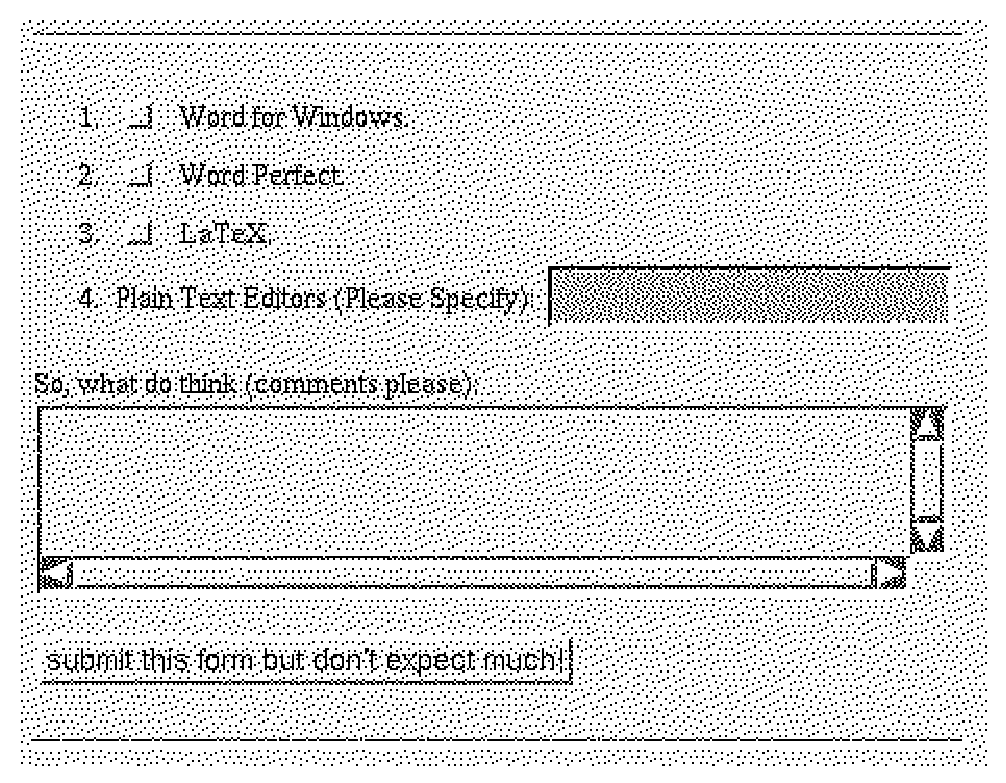
\psfig{file=eform.ps,width=4in}} \\
     Figure: An electronic form. Of course in the online version of this
document the form above would be active.
    \end{center}
\end{figure}
\end{latexonly}

{\bf Warning:} Avoid using LaTeX commands involving counters (e.g.
numbered figures or equations) in conditional text because this may 
disrupt the values of the counters in the electronic version.

% The argument here used to have a \label in its argument which caused
% the ``Contents'' page entry not to be hyperized.
\subsection{Conditional Text}
\label{sec:latexonly}
\index{latexonly} \index{htmlonly}
Conditional text can be specified using the environments {\tt latexonly} and {\tt
htmlonly}. These allow writing parts of a document which are intended
only for electronic delivery or only for paper-based delivery. 

This would be useful for example in adding a long description of a
multimedia resource in the paper version of a document. Such a
description would be redundant in the electronic version, as the user
can have direct access to this resource. 

Here is an example of the use of the {\tt latexonly} environment:

\begin{verbatim}
\begin{latexonly}
\begin{figure}
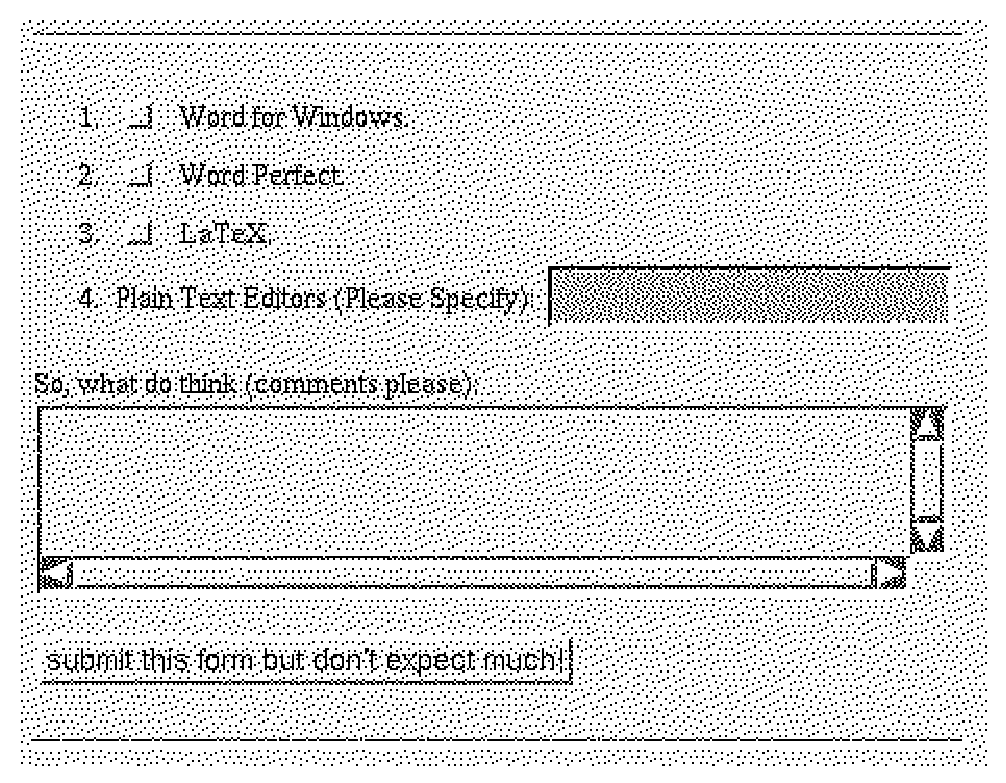
\psfig{file=eform.ps,width=4in}
\caption{An electronic form. Of course in the online version 
of this document the form above would be active!}
\end{figure}
\end{latexonly}
\end{verbatim} 

\subsection{Cross References Shown as ``Hyperized'' Text}

\index{cross-references}
In printed documents cross-references are shown through a {\em numerical
or symbolic indirection} e.g. ``see Figure 1'' (numeric indirection), or
``see section ``Changes'' (symbolic indirection).  \latextohtml can
mirror this mechanism using the same numeric or symbolic references,
or when these are
not appropriate by using iconic references.

In a hypertext document however, cross-references can be shown 
without any indirection just by highlighting a relevant piece of
text. This can make a document more readable as it removes unnecessary
information. 

A single new LaTeX command {\tt hyperref} can be used for
specifying how a cross-reference should appear both in the printed
document and in the hypertext version.

Assuming that the label \verb|sec:cond| is defined somewhere
in a document the command {\tt hyperref} which takes 4 arguments
can be used in the same document as follows:

\index{hyperref} \index{conditional text}
\begin{verbatim}
{\em Is the concept of
\hyperref
% This will be highlighted in the hypertext version
{conditional text}			% argument #1
% This will be shown in the printed version 
% followed by a numeric reference ...      
{conditional text (see Section }  	% argument #2
% ... followed by this text
{ for more information)} 		% argument #3
% This the common label 
{sec:cond}				% argument #4
a good idea? }
\end{verbatim}

Here is how it will be shown: \\
{Is the concept of
\hyperref
% This will be highlighted in the hypertext version
{conditional text}
% This will be shown in the printed version  
% followed by a numeric reference ...      
{conditional text (see Section }  
% ... followed by this text
{ for more information)} 
% This the common label 
{sec:cond}
a good idea? }

\begin{htmlonly}
In the printed version what would appear is: \\
{ Is the concept of conditional text (see Section XXX for more information) a good idea? }
\end{htmlonly}

\begin{latexonly}
In the hypertext version what would appear is:\\
{ Is the concept of \underline{conditional text} a good idea?} \\
Of course \underline{conditional text} would be an active hypertext link.
\end{latexonly}


Another command also defined in {\fn html.sty} is {\tt htmlref} 
which has the same effect as {\tt hyperref} during the conversion to
HTML.
It takes two arguments, some text and a label. In the HTML version the
text will be ``hyperized'' pointing to the label. In the paper version
the text will be shown as it is and the label will be ignored eg

\begin{small}
\begin{verbatim}
With {\tt htmlref} \htmlref{it's easy to make links}{fig:example}.
\end{verbatim}
\end{small}

\begin{htmlonly}
In the HTML version it will be shown as: \\
With {\tt htmlref} \htmlref{it's easy to make links}{fig:example}.
\end{htmlonly}
\begin{latexonly}
In the HTML version it will be shown as: \\
With {\tt htmlref} \underline{it's easy to make links}.
\end{latexonly}


\subsection{Customizing the Navigation Panel}
\index{navigation panel} \label{sec:navpanel}
The navigation panel is the strip containing ``buttons'' and text
that appears at the top
and perhaps at the bottom of each generated page and provides
hypertext
links to other sections of a document. Some of the
options and variables that control whether and where it should appear 
\hyperref{have already been mentioned}{have already been mentioned in 
Section }{}{navoptions}. 


A simple mechanism for appending customized buttons to the navigation
panel is provided by the command {\tt htmladdtonavigation}. This takes
one
argument which \latextohtml appends to the navigation panel. For
example,
\begin{verbatim}
\htmladdtonavigation
   {\htmladdnormallink
      {\htmladdimg{http://server/mybutton.gif}}
      {http://server/link}}
\end{verbatim}
will add an active button {\tt mybutton.gif} pointing to the specified location.


Apart from these facilities it is
also 
possible to specify completely what appears in the navigation panel 
and in what order. As each section is processed, \latextohtml
assigns relevant information to a number of global variables.
These variables are used by the subroutine {\fn navigation$\_$panel}
where the navigation panel is constructed as a string consisting of
these variables and some formatting information. 

This subroutine
can be redefined in a system or a user configuration file ({\fn
LATEX2HTMLDIR/latex2html.config} and {\fn HOME/.latex2html-init} 
respectively). {\em Any combination of text, HTML tags, 
and the variables mentioned below is acceptable}. 

The control panel variables are:

{\bf Iconic links (buttons)}
\begin{itemize}
\item PREVIOUS - points to the previous section 
\item UP  - points up to the "parent" section
\item NEXT - points to the next section
\item NEXT$\_$GROUP - points to the next "group" section
\item PREVIOUS$\_$GROUP - points to the previous "group" section
\item CONTENTS - points to the contents page if there is one
\item INDEX - points to the index page if there is one
\end{itemize}

{\bf Textual links (section titles)}
\begin{itemize}
\item PREVIOUS$\_$TITLE - points to the previous section
\item UP$\_$TITLE  - points up to the "parent" section
\item NEXT$\_$TITLE - points to the next section
\item NEXT$\_$GROUP$\_$TITLE - points to the next "group" section
\item PREVIOUS$\_$GROUP$\_$TITLE - points to the previous "group" section
\end{itemize}

If the corresponding section exists each iconic button will contain an
active link to that section. If the corresponding section does
not exist, the button will be inactive. If the section corresponding
to a textual link does not exist then the link will be empty.

The number of words that appears in each textual link
is controlled by the variable {\fn WORDS$\_$IN$\_$NAVIGATION$\_$PANEL$\_$TITLES}
which may also be changed in the configuration files.

Below is an example of a navigation panel 
(the ``.'' is the Perl string concatenation operator and ``\#''
signifies
a comment).

\begin{small}
\begin{verbatim}
sub navigation_panel {

    #  Start with a horizontal rule (3-d dividing line)
    "<HR> ".			
    
    # Now add few buttons with a space between them
    "$NEXT $UP $PREVIOUS $CONTENTS $INDEX $CUSTOM_BUTTONS" .
	    
    "<BR>\n" .		# Line break
	
    # If ``next'' section exists, add its title to the navigation panel
    ($NEXT_TITLE ? "<B> Next:</B> $NEXT_TITLE\n" : undef) . 
    
\end{verbatim}
\begin{verbatim}
    # Similarly with the ``up'' title ...
    ($UP_TITLE ? "<B>Up:</B> $UP_TITLE\n" : undef) . 
 
    # ... and the ``previous'' title
    ($PREVIOUS_TITLE ? "<B> Previous:</B> $PREVIOUS_TITLE\n" : undef) .
   
    #  Horizontal rule (3-d dividing line) and new paragraph  
    "<HR> <P>\n"		
}
\end{verbatim}
\end{small}

\subsection{Indicating Differences Between Document Versions} 

\latextohtml supports the {\fn changebar.sty} package by David B. Johnson 
(dbj@titan.rice.edu), for 
inserting ``change bars'' in a document in order to indicate 
differences from previous versions. This is a very primitive form of 
version control and there is much scope for improvement.


\subsection{Hypertext Links in Bibliographic References (Citations)}
If a report or a book that is cited (using the {\tt cite}) 
command is available (or there is information about it) on WorldWide
Web then it is possible to add the appropriate hypertext links
in your bibliographic database (the {\fn .bib}) file. 

Here is an example of a bibliographic entry for the original
LaTeX\cite{lamp:latex} book:

\begin{small}
\begin{verbatim}
@book{lamp:latex,
title = "LATEX User's Guide \& Reference Manual",
year = 1986 ,
author = "Leslie Lamport",
Publisher = "Addison-Wesley Publishing Company, Inc.",
note = "Online information on TeX and LaTeX is available at
\htmladdnormallink{http://curia.ucc.ie/info/TeX/menu.html}
{http://curia.ucc.ie/info/TeX/menu.html} and
\htmladdnormallink{http://es-sun2.fernuni-hagen.de/info2html?(latex.info)Top}
{http://es-sun2.fernuni-hagen.de/info2html?(latex.info)Top}"}
\end{verbatim}
\end{small}
No other
modifications are required for this to work - LaTeX and BibTeX 
should work as normal.

For those who use the Harvard style for references
\htmladdnormallinkfoot{there exists a special conversion
add-on package}{http://www.arch.su.edu.au/\~{}peterw/latex/harvard/}.

\subsection{Internationalization}
A special variable {\tt LANGUAGE\_TITLES} 
in the initialization or configuration files determines the language 
in which some section titles will appear. For example setting it to 
\begin{verbatim}
$LANGUAGE_TITLES = ``french'';
\end{verbatim}
will cause LaTeX2HTML to produce ``Table des mati\`{e}res'' instead of
``Table of Contents''.

The only languages currently supported are ``french'' and ``english''
but it is trivial to add support for another language in the
file {\fn latex2html.config}. As a guide here is the entry for 
the French titles:
\begin{verbatim}
sub french_titles {
 $toc_title = "Table des mati\\`eres";	
 $lof_title = "Liste des figures";
 $lot_title = "Liste des tableaux";
 $idx_title = "Index";
 $bib_title = "R\\'ef\\'erences";		
 $info_title = "\\`A propos de ce document..."; 
}
\end{verbatim}

In order to provide full support for another language you may also
want to replace the navigation buttons which come with \latextohtml 
(which are by default in
English)
with your own. As long as the new buttons have the same filenames as the
old ones there should not be a problem.

\subsection{Image Conversion}
\label{imgcon}

\latextohtml converts equations, special accents, external postscript
files, and LaTeX environments it cannot directly translate into 
inlined images. This section describes how it is possible to control
the final appearance of such images. For the purposes of the discussion below,

\begin{description}
\item[{\bf ``small images''}] will refer to equations, special accents and
any other image generating LaTeX commands, while 
\item[{\bf ``figures''}] will
apply  to any image generating LaTeX environments (eg figure, table,
minipage etc).
\end{description}

The size of all ``small images'' depends on a configuration variable
{\tt MATH\_SCALE\_FACTOR} which specifies how much to enlarge or 
reduce them in relation to their original size in the postscript 
version of the document. For example a scale factor of 0.5 will make all 
images half as big while a scale factor of 2 will make them twice as
big.
Larger scale factors result in longer processing times and larger 
intermediate image files. A scale factor will only be effective 
if it is greater than 0. 

The configuration variable {\tt FIGURE\_SCALE\_FACTOR} performs
a similar function for ``figures''. Both of these configuration 
variables are initially set to 1.6.

For finer control, several
parameters affecting the conversion of a single ``figure'' 
can be controlled
with the command {\tt htmlimage} which is defined in {\fn
html.sty}.
The one argument of {\tt htmlimage}
is a string of options separated by commas. The options are
\begin{verbatim}
scale = <scale factor>
external
thumbnail = <scale factor>
map = <image map URL>
\end{verbatim}

The {\tt scale} option allows control over the size of the final
image.

The {\tt external} option will cause the image not to be inlined 
(images are inlined by default). External images will be accessible
via a hypertext link. 

The {\tt thumbnail} option will cause a small inlined image to be 
placed in the caption. The size of the thumbnail depends on the
scale factor. The use of the {\tt thumbnail} option implies
the {\tt external} option. In order to be effective the command
{\tt htmlimage} and its options {\bf must be placed inside the
environment on which it will operate}.

The {\tt map} option will turn the inlined image into an 
\htmladdnormallink{active
image map}{http://wintermute.ncsa.uiuc.edu:8080/map-tutorial/image-maps.html}.

{\bf Example:}
The effect of the LaTeX commands below can be seen in the
\htmlref{thumbnail sketch of Figure}{fig:example} \ref{fig:example}.
\begin{small}
\begin{verbatim}
{\begin{figure}[tbh]
    \htmlimage{thumbnail=0.5}
    \centerline{
    \psfig{file=figure.ps,width=5in}}
    \caption{A sample figure showing part of a page generated by
\latextohtml containing a customized navigation panel (from the
\protect\htmladdnormallinkfoot{CSEP project}
{http://csep1.phy.ornl.gov/csep.html}).}
    \label{fig:example}
\end{figure}}
\end{verbatim}
\end{small}

The {\tt htmlimage} command is also often useful to cancel-out the
effect of the configuration variable {\tt FIGURE\_SCALE\_FACTOR}.
For example to avoid resizing a color screen snap despite 
the value of {\tt FIGURE\_SCALE\_FACTOR} it is possible to 
use {\tt htmlimage\{scale=0\}}.

\subsection{Figures, Tables and Arbitrary Environments}
\index{figures} These are here to show how the translator
handles figures, tables
and other environments. Compare the paper with the online version.

\index{tables}
\begin{table}[h]
\begin{center}
\begin{tabular}{||l|lr||}   \hline
gnats	&	gram	&	\$13.65  \\ \cline{2-3}
	&	each	&        .01	\\ \hline
gnu	& 	stuffed	&        92.50  
                \\  \cline{1-1} \cline{3-3}
emur	&		&	33.33   \\ \hline
armadillo	& frozen	&	8.99 \\ \hline
\end{tabular}
\end{center}
\caption{A sample table taken from \protect\cite{lamp:latex}}
\label{tab}
\end{table}

\index{numbered equations}
Here are some some automatically numbered right-justified equations
\begin{equation} 
\Phi_{l+1,m,n} = (\Phi+h\frac{\partial\Phi}{\partial x} +
\frac{1}{2}h^2\frac{\partial^2\Phi}{\partial x^2} +
\frac{1}{6}h^3\frac{\partial^3\Phi}{\partial x^3} + \ldots)_{l,m,n}
\end{equation}
with some gratuitously \'{a}cc\"{e}nted text in between them.
\begin{eqnarray}  \label{eq:demo}
\frac{\Phi_{l+1,m,n}-2\Phi_{l,m,n}+\Phi_{l-1,m,n}}{h^{2}} +
\frac{\Phi_{l,m+1,n}-2\Phi_{l,m,n}+\Phi_{l,m-1,n}}{h^{2}} + \nonumber \\
\frac{\Phi_{l,m,n+1}-2\Phi_{l,m,n}+\Phi_{l,m,n-1}}{h^{2}} = -I_{l,m,n}(v)
\end{eqnarray}

{\begin{figure}[tbh]
    \htmlimage{thumbnail=0.5}
    \centerline{
    \psfig{file=figure.ps,width=5in}}
    \caption{A sample figure showing part of a page generated by
\latextohtml containing a customized navigation panel (from the
\protect\htmladdnormallinkfoot{CSEP project}
{http://csep1.phy.ornl.gov/csep.html}).}
    \label{fig:example}
\end{figure}}

\section{Getting LaTeX2HTML}
\index{source code}
\begin{flushleft}
The \htmladdnormallink{source code can be obtained 
at http://cbl.leeds.ac.uk/nikos/tex2html/latex2html.tar.}
{http://cbl.leeds.ac.uk/nikos/tex2html/latex2html.tar}
or \htmladdnormallink{as a compressed archive at http://cbl.leeds.ac.uk/nikos/tex2html/latex2html.tar-gz}{http://cbl.leeds.ac.uk/nikos/tex2html/latex2html.tar-gz}
The source code is also available 
via anonymous FTP at 
\htmladdnormallink{ftp://ftp.tex.ac.uk/pub/archive/support/latex2html}{ftp://ftp.tex.ac.uk/pub/archive/support/latex2html}
or
\htmladdnormallink{ftp://sunsite.unc.edu/pub/packages/infosystems/WWW/tools/translators/latex2html}{ftp://sunsite.unc.edu/pub/packages/infosystems/WWW/tools/translators/latex2html}.
Other FTP sites nearer to you can be found using {\fn Archie}
at
\htmladdnormallink{http://hoohoo.ncsa.uiuc.edu/archie.html}{http://hoohoo.ncsa.uiuc.edu/archie.html}
or 
\htmladdnormallink{http://www.pvv.unit.no/archie/}{http://www.pvv.unit.no/archie/}
(faster).

{\bf Warning:} Some FTP sites may not carry the latest version.

Updates and patches are posted on the \latextohtml server at
\htmladdnormallink{http://cbl.leeds.ac.uk/nikos/tex2html/doc/latex2html/latex2html.html}{http://cbl.leeds.ac.uk/nikos/tex2html/doc/latex2html/latex2html.html}

\end{flushleft}

If you get the {\tt tar} version, save it into a file, say {\tt latex2html.tar}
and then extract the files with 
\begin{verbatim}
% tar xvf latex2html.tar
\end{verbatim} 

You should then have the following:
\begin{itemize}
\item A {\fn README} file.
\item A {\fn Changes} file.
\item The {\fn latex2html} Perl program.
\item A \index{texexpand} {\fn texexpand} Perl program \footnote{Written 
by Robert S. Thau $<$rst@edu.mit.ai$>$.}.
\item A {\fn latex2html.config} configuration file.
\item An {\fn install-test} installation and testing Perl script.
\item A {\fn dot.latex2html-init} sample initialization file.
\item A {\fn html.sty} style file.
\item A {\fn pstogif} perl script.
\item Two {\fn pstoppm.ps} files.
\item A {\fn docs/} subdirectory containing a version of this
manual.
\item An {\fn icons/} subdirectory containing various icons.
\item A {\fn styles/} subdirectory containing Perl code for handling
some style files.
\end{itemize}
\section{Requirements}
\index{requirements}
The translator makes use of several utilities all of which 
are freely available on most platforms. \htmladdnormallinkfoot{You may use 
{\fn Archie} to find the source code of any utilities you might need.}
{http://www.pvv.unit.no/archie/}

The requirements for using \latextohtml 
depend on the kind of translation you would like to perform, as follows:

\begin{enumerate}
\item {\bf LaTeX commands but without equations, figures, tables, etc.} \hfill
\begin{itemize}
\item \htmladdnormallink{{\fn Perl}}{ftp://ftp.uu.net/languages/perl/} 
(version 4.0 - RCSfile: perl.c,v - Revision: 4.0.1.8 - Date:
1993/02/05 19:39:30 - Patch level: 36)

{\bf Warning:} You really DO need Perl at patch level 36 or later.
Versions of \latextohtml earlier than 0.7a4 work {\bf only} with 
Perl 4 at patch level 36. Later versions of \latextohtml work 
both with Perl 4 at patch level 36 and Perl 5. {\bf No} version 
of \latextohtml will work  with Perl 4 at earlier patch levels.

\item {\fn DBM} or {\fn NDBM}, the Unix DataBase Management system.
\end{itemize}

\item {\bf LaTeX commands with equations, figures, tables, etc.} \\
As above plus
\begin{itemize}
\item {\fn latex},
\item  \htmladdnormallink{{\fn dvips}}
{ftp://ftp.tex.ac.uk/pub/archive/dviware/dvips}
(version  5.516 or later) or {\fn dvipsk}.
\item {\fn gs} (Ghostscript version 2.6.1 or later). 
\item The \htmladdnormallink{{\fn
pbmplus}}{ftp://ftp.x.org/R5contrib/}
OR \htmladdnormallink{{\fn
netpbm}}{ftp://ftp.x.org/R5contrib/}
library.
Some of the filters in those libraries are used during the postscript to
GIF conversion. 
\end{itemize}

\item 
{\bf \htmladdnormallinkfoot{Transparent inlined images}{http://melmac.corp.harris.com/transparent\_images.html}}\\
If you dislike the ugly white background color of the
generated inlined images then you should get either 
the {\fn netpbm} library (instead of the older {\fn pbmplus}) OR
install the
\htmladdnormallinkfoot{{\fn
giftrans}}{ftp://ftp.rz.uni-karlsruhe.de/pub/net/www/tools/giftrans.c}
filter by Andreas Ley $<$ley@rz.uni-karlsruhe.de$>$. 
Version 1.10.2 is
known to work without problems but later versions should also be OK.

\end{enumerate} 

If {\fn ghostscript} or the {\fn pbmplus} (or {\fn netpbm}) library are not
available it
is still possible to
use the translator with the {\tt -no\_images} option. 

If you intend to use any of the special features of the translator (see Page \pageref{special})
then you have to include the 
{\fn html.sty} file in any LaTeX documents that use them. 

Because by default the translator makes use of inlined images in the final 
HTML output, it would be better to have a viewer which supports 
the {\tt $<$IMG$>$} tag, such as \htmladdnormallink{NCSA 
Mosaic}{http://www.ncsa.uiuc.edu/SDG/Software/Mosaic/Docs/help-about.html}.
If only a character based browser is available or if you want the
generated
documents to be more portable then the translator can be used
with the 
\hyperref{{\tt -ascii$\_$mode} option}{{\tt -ascii$\_$mode} option (See
Section }{ )}{asciimode}. 

\section{Installing LaTeX2HTML}

To install \latextohtml you {\bf MUST} do the following:

\begin{enumerate}
\item {\bf Specify where Perl is on your system}. \\
In each of the files {\fn latex2html}, {\fn texexpand} {\fn pstogif}
and  {\fn install-test},
modify the first line saying where Perl is on your system. 

Some system administrators do not allow Perl programs to run as shell
scripts. This means that you may not be able to run any of the above
programs. {\em In this case change the first line in each of these
programs from}
\begin{verbatim}
#!/usr/local/bin/perl
\end{verbatim}

{\em to}

\begin{verbatim}
: # *-*-perl-*-*
    eval 'exec perl -S  $0 "$@"'
    if $running_under_some_shell; 
\end{verbatim}

\item {\bf Specify where the external utilities are on your system.} \\
In the file {\fn latex2html.config} give the correct pathnames for 
some directories (the {\fn latex2html} directory and the {\fn 
pbmplus} or {\fn netpbm} library) and some executables ({\fn latex, dvips, gs}). 
Note that it is
possible 
to use \latextohtml even
if you don't have some of the external utilities.

While you're at it you may want to change some of the default 
options in the same file.

\item {\bf Run {\fn install-test}.} \\
This Perl script will make some changes in the {\fn latex2html} file
and then check whether the pathnames to any external utilities
(specified during the previous step) are correct. It will not actually
install the external utilities. 

Don't forget to make {\fn
install-test} executable (using the {\fn chmod} command) before
using it if necessary. You may also need to make the files
{\fn pstogif}, {\fn texexpand} and {\fn latex2html} executable 
if {\fn install-test} fails to do it for you.

If for any reason you have trouble running {\fn install-test}
do not despair. Most of what it does is to do with checking
your installation rather than actually installing anything.
To do a {\bf manual installation} just change the variable
{\tt LATEX2HTMLDIR} in the beginning of the file {\fn latex2html}
to point to the directory where the \latextohtml files can be found.
\end{enumerate}

This is enough for the main installation but you may also 
want to do some of the following:
\begin{itemize}

\item {\bf To use the new LaTeX commands which are defined in {\fn html.sty}:} \\
Make sure that LaTeX knows where the html.sty
file is, either by putting it in the same place as the other style files on
your system, or by changing your TEXINPUTS shell environment variable,
or by copying html.sty in the same directory as your LaTeX source file.

\item {\bf To set up different initialisation files:} \\
For a ``per user'' initialisation file, 
copy the file {\fn dot.latex2html-init} in the home directory
of any user that wants it, modify it according to her preferences and
rename it as {\fn .latex2html-init}. At runtime, both the {\fn 
latex2html.config} file and {\fn \$HOME/.latex2html-init} file will be
loaded, but the latter will take precedence.

You can also set up a ``per directory'' initialisation file by 
copying a version of {\fn .latex2html-init} in each directory you
would like it to be effective. An initialisation file
{\fn /X/Y/Z/.latex2html-init} will take precedence over all other
initialisation files if {\fn /X/Y/Z} is the ``current directory'' when
\latextohtml is invoked.

\item {\bf To make your own local copies of the \latextohtml icons:} \\
Please copy the {\fn icons} subdirectory to a 
place under your WWW tree
where they can be served by your server.
Then modify the value of the {\fn \$ICONSERVER} variable in 
{\fn latex2html.config} accordingly. 

{\bf Warning:} If you cannot do that
bear in mind that these icons will have
to travel from Leeds!!! Also, your documents will depend on our
server being operational in the first place.

\item  {\bf To make your own local copy of the \latextohtml
documentation:} \\
This will also be a good test of your installation. 
To do it run \latextohtml on the file {\fn docs/manual.tex}.
You will get better results if you run LaTeX first on the 
same file in order to create some auxiliary files.

\item {\bf To join the community of \latextohtml users:} \\
More information on a mailing list, discussion archives, bug reporting
forms and more is available at \\
\htmladdnormallink{http://cbl.leeds.ac.uk/nikos/tex2html/doc/latex2html/latex2html.html}
{http://cbl.leeds.ac.uk/nikos/tex2html/doc/latex2html/latex2html.html}
\end{itemize}

\section{Changes from Previous Versions}
The \htmladdnormallink{previous versions of the
translator and some patches}{http://cbl.leeds.ac.uk/nikos/tex2html/previous-versions}
are available. A \htmladdnormallink{detailed list of changes}
{http://cbl.leeds.ac.uk/nikos/tex2html/doc/Changes.txt}
which includes full credits to all who have contributed 
bug fixes or other code is also available with the
\latextohtml distribution in the file {\fn Changes}.


\subsection{Changes upto v95}
\begin{description}
\item[{\bf Much improved inlined equation baseline alignment!}]
(Thanks to Mark Segal $<$segal@spud.asd.sgi.com$>$)
Inlined equation bitmaps are now aligned correctly depending 
on whether they contain subscripts, superscripts etc. 
\item[{\bf Support for internationalization}]
(Thanks to Martin Boyer $<$gamin@ireq-robot.hydro.qc.ca$>$)
A global variable {\tt LANGUAGE\_TITLES} can now be used to change the
language in which some section titles (eg ``Table of Contents'') are
printed. It is also very easy to add support for more languages.
\item[{\bf Compatibility with Perl 5}]
\item[{\bf More efficient implementation}]
There has been a major overhaul of the way the source text is parsed
and analysed in order to reduce the memory requirements of this
process.

This has been achieved by spawning off separate Unix processes to deal
with each of the {\tt input}'ed or {\tt include}'d files. As each
process
terminates all the space that it used is reclaimed. 
Asynchronous communication between processes takes place using 
the Unix DataBase Management system (DBM or NDBM) 
which should be present
on your system.

{\bf To take advantage of these changes}, 
it is necessary to split the source text 
into more than one files which can be assembled using the \LaTeX
{\tt input} or {\tt include} commands.


\item[{\bf ``Off-line'' Image Generation}]

Two new options {\tt -no\_images} and {\tt  -images\_only} allow
``off-line'' image conversion. The advantage of using these options is 
that the translation can be allowed to finish even when there are
problems with image conversion. In addition it may be possible to 
fix manually any image conversion problems and then run \latextohtml 
again just to integrate the new images without having to translate
the rest of the text. More instructions on how to do this are
included in the ``Troubleshooting'' section of the \latextohtml
manual.

Can now use either the {\fn pbmplus} or the {\fn netpbm} libary.
If {\fn netpbm} is used then it is no longer necessary to get and
install {\fn giftrans} in order to generate transparent inlined 
images.

Also, a new option {\tt map=$<$image map URL$>$} in the 
command {\tt htmlimage} can turn an included postscript image into an active
image map.

\item[{\bf New options}] \hfill
\begin{description}
\item [-no\_images]
Do not attempt to produce any inlined images. 
The missing images can be generated "off-line" by restarting \latextohtml
with the option {\tt -images\_only}.
\item [-images\_only]
Try and convert any inlined images that were left over from previous
runs of \latextohtml. 
\item [-no\_reuse]
Do {\bf not} reuse images generated during previous translations.
(This will enable the initial interactive session during which the user is
asked whether to reuse the old directory, delete its contents or quit)
\item [-no\_subdir]
Place the generated HTML files  in the 
current directory. The default behaviour is to create (or reuse)
another file directory.
\item [-ps\_images]
Use links to external postscript images rather than inlined GIF images.
\end{description}
\item[{\bf Several small changes and bug fixes}] \hfill
\begin{itemize}
\item It is no longer necessary to get {\fn Giftrans} if {\fn NETPBM}
is available
\item Fixed problems with support for {\fn german.sty}
\item Fixed problems with multiple bibliographies. Each bibliography
is now treated as a separate section.
\item Added support for ``dotless i's and j's''.
\item  Fixed to resolve figure and table numbers when captions contain
accented characters.
\item Added support for hierarchical indices with duplicate index keys
\item Fixed problem with HTML encodings of ISO-LATIN1 characters   
creeping into converted images of figures and tables.
\item  Added new global variable {\tt PAPERSIZE}
to make it easier to change the default behavior when converting large images
\item A new configuration variable ({\tt TRANSPARENT\_IMAGES}) can be 
used to stop any inlined images generated from "figure" environments
from being transparent.
\item Fixed problem which occurs when {\fn getcwd.pl} is not part of the
Perl library.
\item The option {\tt -address ""} is now valid.
\item Fixed a problem with tables of contents.
\item Fixed problem with the use of the {\tt finger} command when
trying to find out the name of the user.
\item Added some support for {\tt tabbing} environments.
\item HTML heading elements no longer contain other markup.
\item Fixed problem with optional argument in citation commands
\item Added some more support for LaTeX2e.
\item Fixed problem with displayed equations forcing all the remaining
equations to be displayed.
\item Fixed bug with converting postscript images containing more than
256 colors.
\end{itemize}
\end{description}

\subsection{Changes upto v0.6.2}

\begin{description}
\item[{\bf Image Conversion}] \hfill
\begin{itemize}
\item The {\fn pstogif} script has been rewritten in Perl and it
now accepts more options for specifying color depth, scale factors
and pixel density.
\item LaTeX {\tt figure} and other environments are now processed
in 24-bit color.
\item Figure and table captions are now converted into HTML
rather than becoming part of the inlined image. This means that 
any cross-references in the captions will become active.
\item It is now possible to control for each generated image:
\begin{itemize}
\item its size 
\item whether it should be inlined or left as an external image
\item if left as an external image whether it should be accessible
via a \htmlref{{\bf generated thumbnail sketch}}{fig:example}
or a textual hypertext link
\end{itemize}
These options are available from a new LaTeX command defined in {\fn
html.sty} called {\fn htmlimage}. 

\item Equations and other inlined images are converted into
transparent GIFs rather than XBMs. {\bf This makes it possible 
to reduced their storage requirements to about 1/6th of what was
previously required!}
\item The default size of equations and other small inlined 
images can be changed
by setting the variable {\tt MATH\_SCALE\_FACTOR} in the
configuration files.
\item The default size of figures, tables, and other large
inlined images can be changed by setting the variable 
{\tt FIGURE\_SCALE\_FACTOR} in the
configuration files.

\item Dvips is now called with the {\tt -M} option which stops it
from invoking {\tt METAFONT}.
\end{itemize}

\item[{\bf Optimization}] \hfill
\begin{itemize}
\item Some effort has gone into reducing the amount of memory required
during conversion. {\bf The impact of these changes can be very
significant}.
In particular, files
containing large numbers of LaTeX commands (eg {\fn .aux} or {\tt .bib}) 
files are handled much better.
\end{itemize}

\item[{\bf Backwards Incompatible Changes}] \hfill
\begin{itemize}
\item The option {\tt -allbitmaps} has been removed. This is no
longer necessary as \latextohtml can now generate transparent
GIF images.
\item The definition of the command {\tt htmladdnormallink} in the 
file {\fn html.sty} has changed and the URL will no longer appear
as a footnote in the paper (DVI) version. The translation of
this command into HTML is {\bf not} affected. 

The previous functionality can be obtained with a new command
{\tt htmladdnormallinkfoot} which will add the URL as a footnote
in the paper version.
\item The script {\fn pstoxbm} is no longer distributed as it is not
used.

\end{itemize}

\item[{\bf Bug Fixes}] \hfill
\begin{itemize}
\item The {\fn install-test} script now recognizes version
numbers correctly and gives better warnings. It also makes
executable any scripts that need to be so. 
\item Stopped using the {\tt nslookup} program to try and guess
e-mail addresses (they were used in signing each generated page). 
This has been replaced with a simple call 
to {\tt finger}.
\item Fixed problem which could cause ``Parameter overflow'' in 
TeX during image conversion.
\item The {\fn texexpand} script has been changed extensively.
Some nasty looping problems are now avoided, and the tracking
down of included files has been improved.
\item Some reported incompatibilities with some Unix shells
(bash,OSF) have been fixed.
\item Displayed equations now appear correctly on separate
lines and are right justified.
\item Fixed bug with nested environments.
\item Fixed problem which caused the wrong numbers to be assigned
to sections with the same titles when the {\tt -show\_section\_titles}
is used (thanks to Brian  Toonen $<$toonen@mcs.anl.gov$>$).
\item Fixed problem with the {\tt hyperref} command which
caused the wrong ``hyperized'' text to appear in the final document.
\item {\tt item} optional arguments can now contain one level of
nesting eg {\tt item[[First Choice]]}.
\item Fixed problems with the ``image caching and reuse'' mechanism 
which avoids converting images unnecessarily..
\end{itemize}

\item[{\bf Other Changes}] \hfill
\begin{itemize}
\item LaTeX2HTML now generates $<$meta$>$ HTML tags which can be used
by \htmladdnormallinkfoot{indexing scripts}
{http://www.ai.mit.edu/tools/site-index.html}
 which generate information for the \htmladdnormallinkfoot{ALIWEB}
{http://web.nexor.co.uk/aliweb/bin/aliwebsimple.pl} 
search and retrieval tool. The information in the $<$meta$>$ tags
contains
the title of each separate HTML file. 
\item A new configuration variable {\tt DEBUG} can be used to preserve
intermediate files for debugging. 
\item Some problems with respect to compatibility with the HTML2.0 
standard have been addressed. No more ``unquoted attribute value literals''.
\item All the navigation icons are now ``lynx friendly''; their
{\tt ALT} attribute now has a meaningful value.
\item A new LaTeX command {\fn htmlref} makes it a lot simpler
to create hypertext links intended only for the HTML version of
the document.
\item {\fn DVIPSK} is now recognized by the installation script
\item Added support for the {\fn changebar.sty} file by 
David B. Johnson (dbj@titan.rice.edu).
\item It is no longer necessary to add style file names into the 
{\tt DONT\_INCLUDE} variable as \latextohtml now does not
attempt to translate file included files ending in {\tt .sty}.
\item The small invisible bitmaps that used to mark anchors have been
replaced with the invisible character \verb|&#160;|.
\item It is no longer necessary to use full pathnames when
including external postscript files.
\item If a file {\fn .latex2html-init} is found in the ``current
directory'' then this will be loaded automatically after loading the
other default configuration files.
\item Changed the naming convention of generated HTML files. The
``top'' document is {\fn $<$FILE$>$.html} as before but all other ``nodes''
are named {\fn nodeN.html} where {\fn N} is an integer. Also, the file
containing
the footnotes is now called {\fn footnode.html}.
\item A special extension to \latextohtml for those who use the 
Harvard style for references can be obtained from
\htmladdnormallink{http://www.arch.su.edu.au/\~{}peterw/latex/harvard/}{http://www.arch.su.edu.au/\~{}peterw/latex/harvard/}.
\end{itemize}
\end{description}


\subsection{Changes upto v0.5.3}
\begin{itemize}
\item The files {\fn LATEX2HTMLDIR/styles/german.perl} and 
{\fn LATEX2HTMLDIR/styles/makeidx.perl} have been fixed
so that they are consistent with changes in the main script.
\item A problem with disappearing spaces after some equations
and other environments has been fixed.
\end{itemize}
\subsection{Changes upto v0.5.1}
\begin{description}
\item[{\bf Navigation Panel}]
The \hyperref{navigation panel}{navigation panel (see section
}{)}{sec:navpanel}
is now fully configurable and much better looking.
\item[{\bf Automatic Signatures}]
The signatures at the bottom of each page are now constructed
using {\fn nslookup} (Thanks to Alberto Accomazzi
$<$alberto@cfa.harvard.edu$>$)
\item[{\bf Numerous fixes including...}] \hfill
\begin{itemize}
\item ``dead'' {\fn next$\_$page} buttons when the {\fn -split} option
was used, and
\item internal \latextohtml markers appearing in section titles.
\end{itemize}
\end{description}

\subsection{Changes upto v0.4}
\begin{description}
\item[{\bf Accents and Special Characters}]
LaTeX accent commands, special characters and accent commands defined
in {\fn german.sty} are translated to equivalent ISO-LATIN-1
characters when that is possible (partly thanks to code supplied
by Franz Vojik $<$vojik@de.tu-muenchen.informatik$>$).
\item[{\bf Auto-loading of Style-Specific Code}]
The translator now supports a 
\hyperref{mechanism for including Perl code extensions}{mechanism for
including Perl code extensions (see Section }{)}{sec:sty}
which are specific to particular style files. 


This mechanism will help to keep the core script smaller as well as make
it easier for others to contribute and share solutions on  
how to translate specific style files. The current distribution includes the files
{\fn german.perl}, {\fn french.perl}, {\fn html.perl} and {\fn makeidx.perl}.
\item[{\bf Installation and Testing}]
To make it easier to install the translator for more than one user
there is now a configuration file ({\fn
LATEX2HTMLDIR/latex2html.config}) which contains installation specific 
information and default values for the various options. 
This makes it unnecessary to have a {\fn HOME/.latex2html-init} for
each user.
If a user does have a  {\fn HOME/.latex2html-init} then this will be
loaded after {\fn
LATEX2HTMLDIR/latex2html.config}.

A new Perl script ({\fn install-test}) is now available with the distribution
which will install the translator, and then perform some tests on the
availability
of some external
programs giving, appropriate warnings.
\item[{\bf Navigation Panel Extensions}]
The following new links have been added to the navigation panel which
appears in each page
(where this is appropriate):
\begin{itemize}
\item a link to the next ``logical'' page (this allows reading each
page in the same order as with a paper-based version - as opposed to
structure navigation)
\item a link to the previous ``logical'' page 
\item a link to the table of contents
\item a link to the index 
\end{itemize}
\item[{\bf HTML Style File Extensions}]
The HTML style file {\fn html.sty} now includes definitions of new 
environments for:
\begin{description}
\item[Inclusion of Raw HTML]
A new LaTeX environment {\tt rawhtml} allows
arbitrary
HTML tags to be included in a LaTeX document. This is useful for
taking
advantage of HTML+ features as they become available (e.g. interactive
forms).
The HTML commands are ignored when producing the DVI version of the
document.
\label{sec:cond}
\item[Conditional Text]
The new environments {\tt latexonly} and {\tt htmlonly} allow their
contents to appear only in final DVI or in the HTML version of a
document respectively. 

A new command {\tt hyperref} can be used to specify the way in
which cross-references should be shown in the DVI version and the
HTML version of the document.
\end{description}
\item[{\bf Right Justification of Equations}]
The translator
adds enough whitespace at the beginning of each equation bitmap
to push it to the right-hand margin. The width of each line can be
set in the configuration file using the variable {\tt LINE$\_$WIDTH}.
\item[{\bf Inlined Images}]
All inlined images are now generated by calling {\tt latex} and {\fn
dvips} only once
at the end of the conversion process (but each generated image still
has to be filtered individually). Also, a warning is given if an 
image cannot be converted.
\item[{\bf Numeric Labels}]
The original (LaTeX generated) numeric labels are used instead of
the arrow navigation icon for cross-references where possible.
To do this the translator uses the information in the 
{\fn aux} file which is generated by \LaTeX. If the {\fn aux} file
is out of date a warning is given.
\item[{\bf New Options}] \hfill
\begin{description}
\item[{\tt -auto$\_$navigation}]
This puts a navigation panel 
at the top of each page as usual. But if the page exceeds a
user-settable  
number of words (the default is 450 words) 
then a navigation panel is also placed at the end of
the page. This option is active by default.
\item[{\tt -index$\_$in$\_$navigation}]
Adds a link to the index in the navigation panel.
\item[{\tt -contents$\_$in$\_$navigation}]
Adds a link to the table of contents in the navigation panel.
\item[{\tt -next$\_$page$\_$in$\_$navigation}]
Adds a link to the next ``logical'' page in the navigation panel.
\item[{\tt -previous$\_$page$\_$in$\_$navigation}]
Adds a link to the previous ``logical'' page in the navigation panel.
\item[{\tt -bottom$\_$navigation}]
This puts a navigation panel at the bottom of each page.
\item[{\tt -top$\_$navigation}]
This puts a navigation panel at the top of each page (the default).
\item[{\tt -show$\_$section$\_$numbers}]
This allows each section (page) title to be numbered in the same 
way that it would be numbered by \LaTeX. This requires 
an up to date {\fn aux} file (generated by running \LaTeX) and that 
each title is unique. If the {\fn aux} file is not up to date then a 
warning is given.
Unfortunately if 
the title contains inlined images the numbering for that title will
be lost. 
\item[{\tt -reuse}]
This allows images generated during previous invocations of
the translator to be ``reused'' without going through the initial 
interactive session. The same behavior is obtained by setting
the variable {\tt REUSE} to 1 (the default) in the configuration file.
Note that images which may depend on contextual information (e.g. numerical
labels) cannot be reused and are always re-generated. 
\end{description}
\item[{\bf Bug Fixes and Minor Changes}] \hfill
\begin{itemize}
\item The links from the table of contents in single page documents (created using
the option {\tt -split 0}) is now working as expected.
\item Newlines are translated to the $<$BR$>$ tag.
\item Fixed some problems in dealing with new command macros.
\item {\fn texexpand} now respects commented {\tt input} and {\tt
include} commands. Also (thanks to Franz Vojik
$<$vojik@de.tu-muenchen.informatik$>$), it 
now looks in subdirectories when expanding
files.
\item The ALIGN attribute of inlined images is now BOTTOM instead of
TOP.
\item Fixed problem with the environment variable {\tt TEXINPUTS}.
\item Added some support for optional user-defined labels (bullets) in
list environments.
\end{itemize}
\end{description}

More details on all the changes are available in the file 
{\fn LATEX2HTMLDIR/Changes}.

\subsection{Changes upto v0.3.1}
These changes are mostly due to patches contributed by Robert S. Thau
$<$rst@ai.mit.edu$>$:
\begin{itemize}
\item Nested environments with the same name are now dealt with
properly.
\item Commands that are passed to LaTeX for processing which have 
environments in their arguments (e.g. a {\tt parbox} command which 
an {\tt itemize} environment as an argument) are now
processed correctly. A general mechanism for users to 
specify the syntax of commands that should be passed to LaTeX 
is described in Page \pageref{pass}.
\item Fixed a problem with recognizing the {\tt special} command.
\item Fixed bug in the generation of the index.
\end{itemize}

\subsection{Changes upto v0.3}
\begin{description}
\item [{\bf Image Recycling}]
Images for equations, tables, figures, special characters etc. generated by
the translator are recognised  during subsequent runs.
The user is then asked whether old images should be reused
(or whether the old images should be deleted and regenerated).
This offers tremendous improvements in speed after an initial
successful translation.

\item [{\bf Cross-References Between (Local or Remote) Documents}]
Cross-references between 
two or more documents (possibly on remote locations) can be
established via symbolic labels
which are independent of the physical realisation of these documents. 

Such cross-references will be maintained with a simple
re-translation\footnote{This is true for documents under the same
server but for remote documents a little more is required (see 
the \hyperref{example}{example in Section}{}{crossrefs})}
even after one or more of the documents have been broken into
different physical parts or moved.

The mechanism is based on the 
\hyperref{new commands}{new commands (see Section }{ )}{external}
{\tt externallabels} and {\tt externalref} which are an extension of the simple 
{\tt label-ref} pairs. 

\item [{\bf New Options}] \hfill
\begin{description}
\item [{\tt external$\_$images}] This provides hypertext links to where
generated images (for equations, tables, figures etc) are stored
externally. (The default is to ``inline'' generated images in the main body 
of the text.)
\item [{\tt ascii$\_$mode}] This switches all the navigation icons to their
ascii equivalents. Also generated images are stored externally as with the 
{\tt external$\_$images} option above. The {\tt ascii$\_$mode} option
makes documents more portable as it allows them to be
viewed on browsers that do not support inlined images.
\end{description}
\item [{\bf Special Command Style File}] A style file \htmladdnormallink{{\fn html.sty}} 
{http://cbl.leeds.ac.uk/nikos/tex2html/doc/html.sty.txt} is now included in the
distribution. This contains the definitions (syntax) of some 
special LaTeX commands mainly for providing external hypertext
links.
This should be included in LaTeX files that use the any 
\hyperref{hypermedia extensions}{hypermedia extensions (see Section}{ )}{special}.

\item [{\bf Minor Changes and Bug Fixes}] \hfill
\begin{itemize}
\item Equations, equation arrays and theorems are now numbered
correctly even when they are individually passed to LaTeX for
processing.
\item Fixed problem with {\tt label} commands appearing in section
headings.
\item Fixed problems with verbatim environments, bibliography items,
generated file names, the options {\tt nolatex} and {\tt
no$\_$navigation}, the {\tt thanks command}, the name of an HTML tag
($<$HEAD$>$), 
\item The appearance of footnotes has been improved.
\item Some inconsistencies in the {\fn pstoxbm} and {\fn pstogif}
 scripts have been fixed.  
\item Parts of the documentation have been rewritten, restructured and
some new sections have been added. 
\end{itemize}
\end{description}

{\bf The following were contributed by Robert S. Thau
$<$rst@ai.mit.edu$>$:}

\begin{description}
\item [{\bf New Texexpand}]
This fixes problems with the standard version and 
handles the inclusion of style files which need to processed by the 
translator. Appropriate modifications to the main script were also 
made to work with new version of {\fn texexpand}. 

\item [{\bf Handling of Raw \TeX}]
Added support for simple raw TeX commands such as  
{\tt special} and simple instances of {\tt def}\footnote{Where
``simple'' is defined roughly 
as ``they could have used {\tt newcommand}, but didn't''.}. 
For the messier cases, 
the definition is scooped up and moved to the preamble.  This allows 
the translator to handle the simple, but nonstandard, postscript figure inclusion
macros as well as an awful lot of other stuff done with gratuitous 
{\tt defs}.
\item [{\bf More Options}] \hfill
\begin{description}
\item [{\tt dont$\_$include}]
This can be used  to specify style files that
should not be included in the translation.
\end{description}
\item [{\bf Other Changes}] \hfill
\begin{itemize} 
\item Added support for nested math mode expressions and general
list environments in order to handle {\em the document from Hell!!!}.
\item Fixed problems in the translation of 
bibitems, the substitution of macro definitions, and the processing of
unrecognized commands in the preamble.
\end{itemize}
\end{description}
\subsection{Changes upto v0.2}
\begin{itemize}
\item Added a command line option
to switch off the navigation links
at the top of each page.
\item The navigation icons are now part of the distribution.
\item Added a customizable separator between the main body of the text
in a page and the child links from that page.
\item The order of the navigation keywords at the top of each page is
the same as that of the navigation icons.
\item The arguments of {\tt verbatim} environments are now translated
into fixed width fonts.
\item A warning is given if a {\tt bbl} (bibliography) file is 
needed but not found.
\item The installation is now (mostly) done by setting variables in 
just one file.
\item The {\fn pstoxbm} script now uses environment variables
set in the initialization file.
\item Fixed bug in translating sequences of special HTML characters
(e.g. \&, $<$, etc.)
\item Fixed bug in the handling of the \verb|$$|-form of the dislay
math environment.
\item Fixed bug in the handling of the *-forms of environments.
\item Added sections on how to embed hyperlinks in a LaTeX document 
(see Page \pageref{sec:hyper}) and on how to extend the translator
(see Page \pageref{sec:extend}) in the documentation.
\end{itemize}

\subsection{Changes upto v0.1.1}
\begin{itemize}
\item Fixed bug about empty lines being inserted in environments that
cannot tolerate them (e.g. {\tt math}).
\item Changed the format of inlined images coming back from LaTeX
from GIF to XBM. This looks better on grayscale and color monitors.
\item Fixed problem with commands being passed on to LaTeX  after
their
arguments had been translated (this affects the commands 
{\tt psfig}, {\tt fbox}, {\tt framebox}, and {\tt parbox}).
\end{itemize}
\section{Known Problems}
\index{problems} \index{bugs}
Here are some of the problems of the current version:
\begin{description}
\item [{\bf Correctness and Efficiency} \index{efficiency}]
The translator cannot be guaranteed to perform as expected.
Several aspects of the implementation need
optimization and improvement. Apart from possible bugs the translator 
may place heavy demands on your resources.
\item [{\bf Unrecognized Commands and Environments} \index{unrecognized commands}]
Unrecognized commands are ignored and any arguments are left in the
text. Unrecognized environments are passed to LaTeX  and the result is
included in the document as one or more inlined images.
\item [{\bf Cross-references}\index{cross-references}]
References in environments that are passed to LaTeX  for processing
(e.g. a {\tt cite}, or a {\tt ref} command), are not processed
correctly.
{\tt label} commands are handled correctly.
\item[{\bf Order Sensitive Commands}]
Commands which affect global parameters during the translation,
and are sensitive to the order in which they are processed may
not be handled correctly. In particular, counter manipulation
(e.g. {\tt newcounter, setcounter, stepcounter}, etc) 
commands may cause problems.
\item [{\bf Index}\index{index}]
The translator generates its own index by saving the arguments  of 
the {\tt index} command. The contents of the {\tt theindex}
environment are ignored.
\item[{\bf New Definitions}\index{new definitions}]
New definitions ({\tt newcommand}, {\tt newenvironment}, {\tt
newtheorem} and {\tt def}),
will not work as expected if they are defined more than once.
Only the last definition will be used throughout the document.
\item [{\bf Scope of declarations and environments}]
If the scope of a declaration or environment crosses section
boundaries, then the output may not be as expected, because each
section is processed independently.
\end{description}

\section{Troubleshooting}
\index{debugging} \index{problems} \index{fixes}
Here are some curable symptoms:

\begin{description}
\item [{\bf Cannot run any of the Perl programs}]
If your Perl installation is such that Perl programs are not allowed 
to run as shell scripts you may be unable to run  {\fn latex2html}, {\fn texexpand} {\fn pstogif}
and  {\fn install-test}. In this case change the first line in each of these
programs from
\begin{verbatim}
#!/usr/local/bin/perl
\end{verbatim}

{\em to}

\begin{verbatim}
: # *-*-perl-*-*
    eval 'exec perl -S  $0 "$@"'
    if $running_under_some_shell; 
\end{verbatim}

\item [{\bf The {\fn install-test} script gives uninformative error messages}]
If for any reason you have trouble running {\fn install-test}
do not despair. Most of what it does is to do with checking
your installation rather than actually installing anything.
To do a {\bf manual installation} just change the variable
{\tt LATEX2HTMLDIR} in the beginning of the file {\fn latex2html}
to point to the directory where the \latextohtml files can be found.

Also, make sure that the files
{\fn pstogif}, {\fn texexpand} and {\fn latex2html} are executable,
and if necessary use the Unix {\fn chmod} command to make them 
executable.

\item [{\bf It just stops}] Check the style
files that you are using. It is likely that you are using
a style file which contains raw TeX commands. In such a case
start \latextohtml with the option {\tt -dont$\_$include $<$style file
name$>$}. Alternatively, add the name of the style to the variable 
{\tt DONT$\_$INCLUDE} in your
{\fn HOME/.latex2html-init} file. If you don't have such a file then
create one and add the lines:
\begin{verbatim}
$DONT_INCLUDE = "$DONT_INCLUDE" . ":<style file name>";
1; 	# This must be the last line
\end{verbatim}

Another reason why \latextohtml might stop is that the LaTeX source
file itself contains raw TeX commands. In this case you may 
put such commands inside a 
\hyperref{{\tt latexonly}}{{\tt latexonly (see Section }}{)}{sec:latexonly}
environment.

\item [{\bf Perl cannot parse the {\fn latex2html} script}]
Update your Perl to patch level 36. You can check which version of
Perl you are using by invoking Perl with the {\tt -v} option.
Earlier versions of Perl than that shown above
have caused problems due
to tighter control over syntax.
\item [{\bf It crashes (dumps core) as soon as it starts \label{perl}}]
Update your Perl 4 to patch level 36 or later (Perl 5).

You can check which version of
Perl you are using by invoking Perl with the {\tt -v} option.


While you wait for your technical support people to upgrade Perl
you could try invoking Perl from within \latextohtml with 
the {\tt -d} (debug) option. Then, when \latextohtml starts, it will
immediately fall into the Perl debugger. To continue just press {\tt
c <CR>}.

\item [{\bf {\fn dvips} complains about incorrect arguments \label{dvips}}]
Please use a version which supports the command line options {\tt -M -S,
-o and -i}. ``Recent'' versions at least after 5.516 do
support them.

\item [{\bf It gives an {\tt Out of memory} message and dies}] 
If you are using version \latextohtml 0.7 or later try splitting your 
source file into more than one files using the \LaTeX\ 
commands {\tt input} or {\tt include}. 
Also, use the {\tt -no\_images} option.

As a last resort you may consider increasing the virtual memory
(swap space) of your machine. As an indication 
of what you might be able to do on your machine,
a very long book (about 1000 printed pages) required about 
24MB of RAM and over 150MB of swap space to convert on a local Sun Sparc ELC
running SunOS 4.1.3.

\item [{\bf It gives ``dbm'' related error messages}]
\latextohtml 0.7 and later requires the
Unix DataBase Management system (DBM or NDBM) in order to run.
This is usually part of each Unix operating system but if you 
don't have it then you may need to get it. \htmladdnormallinkfoot{Use Archie}
{http://www.pvv.unit.no/archie/} to find one.

\item [{\bf The {\tt verb"ABC"} command doesn't work}]
This is a nasty bug. Please use any characters other than quotes eg
{\tt verb+ABC+}

\item [{\bf Cannot get the ``tilde'' (\~{}) to show}]
The trick here is to use the command \verb|\~{}|. 

Alternatively it is possible to use something like \\
\verb|\htmladdnormallink{mylink}
{\begin{rawhtml}http://host/~me/path/file.html\end{rawhtml}}|

or

\verb|\htmladdnormallink{mylink}
{http://host/\%7Eme/path/file.html}| 

{\bf Warning:} Some browsers may not be able to interpret the \verb|%7E|
as a ``tilde'' character.

\item [{\bf Macro definitions don't work correctly}]
As mentioned in other places plain TeX definitions cannot be
converted.
But you may also have problems even when using LaTeX definitions
(with {\tt newcommand} and {\tt newenvironment}) if such definitions
make use of {\it sectioning or verbatim} commands. These are 
handled in a special way by \latextohtml and cannot be used in
macro definitions. 

In general the macro handling mechanism is inefficient and very
fragile. Avoid using macros if possible.

\item [{\bf {\tt input} commands}]
There is a bug in the expansion of {\tt input} commands which causes a problem
when more than one {\tt input} command appear on the same line.
There is no quick fix other than suggesting that you 
insert a newline after {\tt input} commands in the source .tex files.

\item [{\bf {\tt input} commands in verbatim environments}]
These cause problems. There is no fix yet.

\item [{\bf {Optional arguments in description environments}}]
If you have optional arguments for the {\tt item} command in 
a description environment containing nested ``]'' characters then 
these may not show up correctly. To avoid the problem enclose them
in \{\}'s eg \verb+\item[{[nested [angle [brackets] are ok]]}]+

\item [{\bf LaTeX2HTML behaves differently even when you run it on the
same file}]

If you notice any strange side-effects from previous runs of
\latextohtml try using the option {\tt -no\_reuse} and choose 
{\tt (d) } when prompted. This will 
clear any intermediate files generated during previous runs.
Note that this option will disable to image reuse mechanism.

\item [{\bf Cannot convert postscript images which are included
in the LaTeX file}] \hfill \\
It is likely that the macros you are using for including postscript
files (e.g. {\tt epsffile}) are not understood by \latextohtml.
To avoid this problem enclose them in an environment which will
be passed to LaTeX anyway e.g.
\begin{verbatim}
\begin{figure}
\epsffile{<postscript file name>}
\end{figure}
\end{verbatim}

Another reason why this might happen is that your shell 
environment variable 
{\tt TEXINPUTS} is undefined. This is not always 
fatal but if you have problems you can use full
pathnames for included postscript files (even when the postscript
files are in the same directory as the LaTeX source file).
Alternatively try setting TEXINPUTS to ".::". 
With some TeX and LaTeX installations setting TEXINPUTS to 
".::" may cause problems in the normal operation of LaTeX.
If you get errors such as LaTeX complaining that it can no longer find
any style files then you must set TEXINPUTS to 
\verb|"<path to your LaTeX installation>:."|
if you want to use both LaTeX and LaTeX2HTML.

\item [{\bf Some of the inlined images are in the wrong places}]
This happens when any one of the inlined images is more than a page
(paper page) long. This is sometimes the case with very large tables
or large postscript images. In this case you can try specifying 
a larger paper size (eg ``a3'', ``a2'' or even ``a0'') instead of
the default (``a4'') using the LaTeX2HTML variable {\fn PAPERSIZE} 
in the file {\fn latex2html.config}.

Another reason why this may happen is that by default the {\fn dvips} program
reverses the postscript pages it generates. If your {\fn dvips
program}
behaves in this way try changing the line
\verb|$DVIPS = "dvips";| 

to

\verb|$DVIPS = "dvips -r0";|

in the file {\fn latex2html.config}.

\item [{\bf Unacceptable quality of converted images}]
Try changing the size of the image 
(\hyperref{See image conversion}{See Section }{}{imgcon}).

\item [{\bf The bibliographic references are missing}]
Run {\tt latex} and then {\tt bibtex} on the original source file in
order to generate a {\tt bbl} file. \latextohtml requires a {\tt bbl}
in order to generate the references.

\item [{\bf The labels of figures, tables or equations are wrong}]
This can happen if you have used any figures, tables, equations or
any counters inside conditional text i.e. in a {\tt latexonly} 
or a {\tt htmlonly} environment. 

\item [{\bf Problems after changing the configuration files}]
Please make sure that the last line in the configuration files 
(ie {\fn .latex2html-init} and {\fn latex2html.congif}) is:
\begin{verbatim}
1;	# This is the last line
\end{verbatim}
This is a Perl quirk...

\item [{\bf Problems when producing the DVI version \label{htmlsty}}]
If you are using any of the new LaTeX commands which are defined in 
the {\fn html.sty} file make sure that 
{\fn html.sty} file is included e.g. as one of the optional arguments to the 
{\tt documentstyle} command.

Of course you also have to make sure that LaTeX knows where the html.sty
file is, either by putting it in the same place as the other style files on
your system, or by changing your TEXINPUTS shell environment variable\footnote{
If don't know how to do either of these things, copy (or link) html.sty 
to the directory of your LaTeX document...}.

\item [{\bf Some of the fonts are translated incorrectly}]
There is a fault in way the LaTeX scoping rules have been 
interpreted in \latextohtml. Consider this:
\begin{verbatim}
\tt fixed-width font.
\begin{something}
nothing here
\end{something}
default font.
\end{verbatim}
When processed by \LaTeX, the effect of the {\tt tt} command is
delimited
by the beginning of the environment ``something'' so that ``default font'' will
appear in the default font. But \latextohtml will not recognize
``something'' as a delimiter and ``default font'' will appear in the
wrong
font. 

To avoid this problem until it is fixed you may delimit the scope of
some
commands explicitly using \verb|{}|'s i.e.
\begin{verbatim}
{\tt fixed-width font}.
\begin{something}
nothing here
\end{something}
default font.
\end{verbatim}

\item [{\bf You just upgraded to {\fn Ghostscript 3.X} and you can no
longer generate inlined images for equations
etc.}]
If you have a version of \latextohtml later than 0.6.1, go to the
\latextohtml directory and run {\fn install-test} again. This should 
fix it.

With earlier versions of \latextohtml you can fix it by 
replacing the file {\fn pstoppm.ps} in the 
\latextohtml directory with a newer one that accompanies 
{\fn Ghostscript 3.X}. Alterhatively you can avoid using {\fn
pstoppm.ps} 
by changing the way {\tt GS} is invoked in the file {\fn pstogif},
using something like \\
\verb/open (GS, "|$GS -q -sDEVICE=ppmraw  -sOutputFile=$base.ppm $base.ps");/

\item [{\bf Cannot get it to generate inlined images}]
Try a small test file e.g.
\begin{verbatim}
% image-test.tex
\documentstyle{article}
\begin{document}
Some text followed by \fbox{some more text in a box}.
\end{document}
\end{verbatim}

You should see something like:
\begin{verbatim}
This is LaTeX2HTML Version  (Wed Dec 1 1993) by Nikos Drakos, 
Computer Based Learning Unit, University of Leeds.

OPENING /usr/cblelca/nikos/scripts/tex2html/tests/image-test.tex 

Reading ....
Translating ...0/1.....1/1......
Generating images using latex ...
This is TeX, C Version 3.14t3
(12222_images.tex
LaTeX Version 2.09 <7 Dec 1989>


Generating postscript images using dvips ...
This is dvips 5.521 Copyright 1986, 1993 Radical Eye Software
\end{verbatim}
\begin{verbatim}
' TeX output 1993.12.03:1050' -> 12222_image
(-> 12222_image001) <tex.pro>[1] 
Initializing... done.
Ghostscript 2.6.1 (5/28/93)
Copyright (C) 1990-1993 Aladdin Enterprises, Menlo Park, CA.
  All rights reserved.
Ghostscript comes with NO WARRANTY: see the file COPYING for details.
GS>GS>Writing 12222_image001.ppm
GS>pnmcrop: cropping 119 rows off the top
pnmcrop: cropping 961 rows off the bottom
pnmcrop: cropping 208 cols off the left
pnmcrop: cropping 484 cols off the right

Doing section links .....
Done.
\end{verbatim}


If there is a problem somewhere during the conversion from postscript
to GIF you can try to do it manually so that you can find out where
the problem is. Here is one way to do it (Please use the {\fn pstoppm3.ps}
file instead of {\fn pstoppm.ps} if your version of ghostscript is
later than 3.0):

\begin{verbatim}
cblelca% latex image-test.tex
This is TeX, C Version 3.14t3
(image-test.tex
LaTeX Version 2.09 <7 Dec 1989>
(/usr/TeX/tex.lib/inputs//paper.sty
Document Style `paper' <28 Nov 89>.
(/usr/TeX/tex.lib/inputs//pap11.sty) (/usr/TeX/tex.lib/inputs//doublespace.sty)
(/usr/TeX/tex.lib/inputs//smaller.sty)) (/usr/TeX/tex.lib/inputs//psfig.sty
psfig/tex 1.9
)
No file image-test.aux.
[1] (image-test.aux) )
Output written on image-test.dvi (1 page, 652 bytes).
Transcript written on image-test.log.
cblelca% dvips -o image-test.ps image-test.dvi
\end{verbatim}
\begin{verbatim}
This is dvips 5.519 Copyright 1986, 1993 Radical Eye Software
' TeX output 1993.11.12:1412' -> image-test.ps
<tex.pro>. [1] 
cblelca% gs -dNODISPLAY pstoppm.ps
Initializing... done.
Ghostscript 2.6.1 (5/28/93)
Copyright (C) 1990-1993 Aladdin Enterprises, Menlo Park, CA.
  All rights reserved.
Ghostscript comes with NO WARRANTY: see the file COPYING for details.
GS>(image-test) ppm1run 
Writing image-test.ppm
GS>quit
cblelca% pnmcrop image-test.ppm >image-test.crop.ppm
pnmcrop: cropping 61 rows off the top
pnmcrop: cropping 110 rows off the bottom
pnmcrop: cropping 72 cols off the left
pnmcrop: cropping 72 cols off the right
cblelca% ppmtogif image-test.crop.ppm >image-test.gif
\end{verbatim}

\item [{\bf STILL cannot get it to generate inlined images for equations
etc.}]
If you have no problems with the {\fn image-test.tex} file but you
still cannot convert the images in some of your files 
have a look in the directory of the generated
HTML files for two files {\fn images.tex} and {\fn images.log}. Do you notice
anything unusual in them? Copy {\fn images.tex} in the directory 
of your original \LaTeX file and run {\fn latex} on {\fn images.tex}.
Can you see any errors in {\fn images.log}? If yes can you fix
{\fn images.tex} to get rid of the errors? After fixing {\fn
images.tex}
you can put it back in the directory of HTML files created by
\latextohtml and run \latextohtml on the original document 
using the option {\tt -images\_only}. 

If you get into a mess try running \latextohtml with the options
{\tt -no\_reuse} and {\tt -no\_images} eg
\begin{verbatim}
cblipca% latex2html -no_reuse -no_images test.tex
This is LaTeX2HTML Version 95 (Tue Nov 29 1994) by Nikos Drakos, 
Computer Based Learning Unit, University of Leeds.

OPENING /tmp_mnt/home/cblelca/nikos/tmp/test.tex 
Cannot create directory /usr/cblelca/nikos/tmp/test: File exists
(r) Reuse the images in the old directory OR
(d) *** DELETE *** /usr/cblelca/nikos/tmp/test AND ITS CONTENTS OR
(q) Quit ?
:d

Reading ...
Processing macros ....+.
Reading test.aux ......................
Translating ...0/1........1/1.....
Writing image file ...

Doing section links .....

*********** WARNINGS ***********

If you are having problems displaying the correct images with Mosaic,
try selecting "Flush Image Cache" from "Options" in the menu-bar 
and then reload the HTML file.

Done.
\end{verbatim}

Then try to have a look 
in the file  {\fn images.tex} (as described earlier) and perhaps fix it.
Once you are happy that {\fn images.tex} is OK run \latextohtml
again with the option {\tt -images\_only}.

The options {\tt no\_reuse, no\_images} and {\tt images\_only}
are available with \latextohtml
version 0.7 or later.

Some problems in displaying the correct inlined images,
may be due to the image caching mechanisms of your browser.
With some browsers a simple ``Reload Current Document'' will be enough
to refresh the images but with others (eg Mosaic) you may need
to request for the cache to be refreshed. With Mosaic try 
selecting "Flush Image Cache" from "Options" in the menu-bar 
and then reload the HTML file.


\item [{\bf It cannot do slides, memos, etc, ...}] 
If you use {\tt slitex} you can go a long way just by replacing 
the {\tt slides} argument of the {\tt documentstyle} command with 
something like {\tt article} just before using \latextohtml.
One problem may be that all your slides will end up in the  same HTML 
file.
If you use {\fn lslide.sty} you may get much better results 
(\htmladdnormallinkfoot{use Archie}
{http://www.pvv.unit.no/archie/} to find this or any other
style files).
\end{description}


\section{Support and More Information}

Announcements, discussion archives, bug reporting forms, archives and
more are kept at the \latextohtml home at \\
\htmladdnormallink{http://cbl.leeds.ac.uk/nikos/tex2html/doc/latex2html/latex2html.html}{http://cbl.leeds.ac.uk/nikos/tex2html/doc/latex2html/latex2html.html}.

A \htmladdnormallink{\latextohtml mailing list}{mailto:latex2html-request@mcs.anl.gov} has been set up at the
Argonne National Labs (thanks to Ian Foster 
$<$itf@mcs.anl.gov$>$ and Bob Olson $<$olson@mcs.anl.gov$>$). The
\htmladdnormallinkfoot{\latextohtml mailing list
archive}{http://cbl.leeds.ac.uk/nikos/tex2html/doc/mail/mail.html} is
available.

To join send a message to: \\
{\tt latex2html-request@mcs.anl.gov}  \\
with the contents \\
{\tt subscribe}

To be removed from the list send a message to: \\
{\tt latex2html-request@mcs.anl.gov}  \\
with the contents \\
{\tt unsubscribe}.

\section{General License Agreement and Lack of Warranty}
This software is distributed in the hope that it will be useful
but {\bf without any warranty}. The author(s) do not accept responsibility 
to anyone for the consequences of using it or for whether it serves 
any particular purpose or works at all. No warranty is made about 
the software or its performance. 
 
Use and copying of this software and the preparation of derivative
works based on this software are permitted, so long as the following
conditions are met:
\begin{itemize}
\item The copyright notice and this entire notice are included intact
and prominently carried on all copies and supporting documentation.
\item No fees or compensation are charged for use, copies, or
access to this software. You may charge a nominal
distribution fee for the physical act of transferring a
copy, but you may not charge for the program itself. 
\item If you modify this software, you must cause the modified
file(s) to carry prominent notices (a Change Log)
describing the changes, who made the changes, and the date
of those changes.
\item  Any work distributed or published that in whole or in part
contains or is a derivative of this software or any part 
thereof is subject to the terms of this agreement. The 
aggregation of another unrelated program with this software
or its derivative on a volume of storage or distribution
medium does not bring the other program under the scope
of these terms.
\end{itemize}
 
This software is made available {\bf as is}, and is distributed without 
warranty of any kind, either expressed or implied.
In no event will the author(s) or their institutions be liable to you
for damages, including lost profits, lost monies, or other special,
incidental or consequential damages arising out of or in connection
with the use or inability to use (including but not limited to loss of
data or data being rendered inaccurate or losses sustained by third
parties or a failure of the program to operate as documented) the 
program, even if you have been advised of the possibility of such
damages, or for any claim by any other party, whether in an action of
contract, negligence, or other tortious action.

\index{copyright}
The \latextohtml translator is written by Nikos Drakos, 
Computer Based Learning Unit,  University of Leeds,  Leeds,  LS2 9JT.
Copyright \copyright 1993, 1994, 1995. All rights reserved.
 
\section{Credits}
Several people have contributed suggestions, ideas, solutions, support
and encouragement. Some of these are Roderick Williams, Ana Maria
Paiva, Jamil Sawar and Andrew Cole here at the Computer Based Learning Unit.

The idea of splitting LaTeX  files
into more than one components linked with hyperlinks was first
implemented in Perl by Toni Lantunen at CERN.
Thanks to Robert Cailliau $<$cailliau@cernnext.cern.ch$>$
of the WorldWide Web Project also at CERN 
for giving me access to the source code and documentation (although no
part of the original design or the actual code has been used).

Robert S. Thau $<$rst@edu.mit.ai$>$ has contributed the new version of
{\fn texexpand}. Also, in order to translate the {\em document 
from hell} (!!!) he has extended the translator to handle {\tt def}
commands, nested math-mode commands, and has fixed several bugs.

The {\fn pstogif} script 
uses the {\fn pstoppm.ps} postscript program originally written by
Phillip Conrad (Perfect Byte, Inc.) and modified by L. Peter Deutsch 
(Aladdin Enterprises).

The idea of using existing symbolic labels to provide cross-references
between documents was first conceived during discussions with 
Roderick Williams $<$rodw@cbl.leeds.ac.uk$>$.
Eric Carroll $<$eric@ca.utoronto.utcc.enfm$>$ suggested providing
a command like {\tt hyperref}. Franz Vojik
$<$vojik@de.tu-muenchen.informatik$>$
provided the basic mechanism for handling foreign accents.
The {\tt -auto$\_$navigation} option was based on an idea by
Todd $<$little@com.dec.enet.nuts2u$>$.
Axel Belinfante $<$Axel.Belinfante@cs.utwente.nl$>$ provided the
code in the {\fn makeidx.perl} file as well as numerous suggestions
and bug reports. 

Verena Umar $<$verena@edu.vanderbilt.cas.compsci$>$ 
(\htmladdnormallink{Computer Science
Education Project}{http://csep1.phy.ornl.gov/csep.html}) has been a very
patient tester of some early versions of \latextohtml
and many of the current features are a result of her 
suggestions. 

Thanks to (thanks to Ian Foster 
$<$itf@mcs.anl.gov$>$ and Bob Olson $<$olson@mcs.anl.gov$>$) at the
Argonne National Labs for setting up the
\htmladdnormallinkfoot{\latextohtml mailing list}{http://cbl.leeds.ac.uk/nikos/tex2html/doc/mail/mail.html}.

Many others, too many to mention, 
have contributed bug reports, fixes, and other suggestions. Keep them coming!

\bibliographystyle{plain}

\begin{thebibliography}{1}
\bibitem{lamp:latex}
Leslie Lamport.
\newblock {\em LATEX User's Guide \& Reference Manual}.
\newblock Addison-Wesley Publishing Company, Inc., 1986.
\newblock Online information on TeX and LaTeX is available at
  \htmladdnormallink{http://curia.ucc.ie/info/TeX/menu.html}{http://curia.ucc.%
ie/info/TeX/menu.html} and
  \htmladdnormallink{http://es-sun2.fernuni-hagen.de/info2html?(latex.info)Top%
}{http://es-sun2.fernuni-hagen.de/info2html?(latex.info)Top}.
\end{thebibliography}


\begin{theindex}
\documentstyle[psfig,html]{article}

% use %sort -f -u manual.idx > manual.index for a primitive index

%%%%%%%%%%%%%%%%%%% No changes beyond this point %%%%%%%%%%%%%%%%%%%%%%%%%%%%%

\makeindex
%\psdraft
% Transforms the \indexentry generated by \makeindex in the concepts.idx
% file into a form understood by the theindex environment.
% See below on h	ow to produce an index.
\newcommand{\latextohtml}{ {\bf LaTeX}{2}{\tt{HTML}} }
\newcommand{\fn}{\tt}	% file names
\newcommand{\indexentry}[2]
   {\item #1 #2}

\setlength{\textwidth}{5.5in}
\addtolength{\oddsidemargin}{-1in}
\addtolength{\evensidemargin}{-1in}
\begin{document}
\sloppy
\title{The LaTeX2HTML Translator}
\author{Nikos Drakos,\\ Computer Based Learning Unit,\\ University of
Leeds.}
\date{\today}
\maketitle 

\centerline{This document accompanies LaTeX2HTML Version 95}

\begin{htmlonly}
A \htmladdnormallink{postscript
version}{http://cbl.leeds.ac.uk/nikos/tex2html/doc/manual.ps}
is available. \index{postscript version}

{\bf Warning:} The contents of this document are likely to change.
It is advisable not to use links to any pages other than the first
page (this page).
\end{htmlonly}

\begin{abstract} 
\latextohtml is a conversion tool that allows documents
written in LaTeX to become part of the WorldWide Web.
In addition, it offers an easy migration path towards
authoring complex hypermedia documents using
familiar word-processing concepts.

\latextohtml replicates the basic structure of a LaTeX document 
as a set of interconnected HTML files which can be explored using
automatically generated navigation panels. 
The cross-references, citations, footnotes, the table of contents and the lists
of figures and tables, are also translated into hypertext links. Formatting
information which has equivalent ``tags'' in HTML (lists, quotes, paragraph
breaks, type styles, etc.) is also converted appropriately. 
The remaining heavily formatted items
such as mathematical equations, pictures or tables are converted to images
which are placed automatically at the correct positions in the
final HTML document.

\latextohtml extends LaTeX by supporting arbitrary hypertext links 
and symbolic cross-references between evolving 
remote documents. It also allows the specification
of {\em conditional text} and the inclusion of raw HTML commands.
These hypermedia extensions to LaTeX are available as 
new commands and environments from with a LaTeX document.

This document presents the main features of \latextohtml, and
describes how to obtain, install, and use it.
\end{abstract}

\pagebreak
\tableofcontents
\listoffigures
\listoftables

\pagebreak

\section{Overview}
\index{overview}
This document describes the \latextohtml translator which:

\begin{itemize}
\item breaks up a document into one or more components as specified
by the user\footnote{The user can specify the {\em depth} at which 
the document should not be broken up any further.},
\item provides optional, customizable iconic navigation
panels on every page which contain links to other parts of the
document, or other documents,
\index{inlined equations}
\item hadles inlined equations ( \(\sum_{i=1}^{n} x_{i} =
\int_{0}^{1} f \)), handles equation alignment ($A_{B_{C+D}}$), 
right-justified numbered equations
(see equation \ref{eq:demo}), tables (see Table \ref{tab}), or
figures (see Figure \ref{fig:example}),
and {\em any arbitrary environment}\footnote{These are
passed to LaTeX and then converted to images which are either included
in the document or are made available through hypertext links.},

\item 
figures or tables can be arbitrarily scaled and shown either as
inlined images or ``thumbnail'' sketches
\item can produce output suitable for browsers that support inlined
images or character based browsers (as specified by the user),
\item handles definitions of new commands, environments, and theorems
even when these are defined in external style files\footnote{
This allows the definition of HTML macros in LaTeX  !},
\item handles footnotes\footnote{Like this!}, tables of contents, lists
of figures and tables, bibliographies, and can generate an
\index{index} index,
\item translates cross-references into hyperlinks and 
extends the LaTeX cross-referencing mechanism to work
not just within a document but {\em between documents} which may
reside in remote locations, \index{ISO-LATIN-1}
\item translates LaTeX accent and special character commands
(e.g. \. {A} \O \"o \pounds \copyright \P) to
the equivalent ISO-LATIN-1 character set where possible,
\item recognizes hypertext links (to multimedia resources or
arbitrary internet services such as sound/video/ftp/http/news) and
links which invoke arbitrary program scripts,
all expressed as LaTeX commands,
\item recognizes {\em conditional text}  which is intended only for
the hypertext version, or only for the paper (DVI) version,
\item can include raw HTML in a LaTeX document (e.g. in order to
specify interactive forms),
\item can deal sensibly at least with the {\em Common LaTeX  commands}
summarized at the back of the LaTeX  blue book \cite{lamp:latex},
\item will try and translate any document with embedded LaTeX commands 
irrespective of whether it is complete or syntactically legal.
\end{itemize}

A selection of documents illustrating the different contexts in 
which \latextohtml has been used is available at \\
\htmladdnormallink{http://cbl.leeds.ac.uk/nikos/tex2html/doc/latex2html/latex2html.html}{http://cbl.leeds.ac.uk/nikos/tex2html/doc/latex2html/latex2html.html}.

\section{User Manual}
\index{man page} \label{sec:man}

To use \latextohtml simply type {\fn latex2html $<$file$>$.tex}. This 
will create a new directory called {\tt file} which will contain 
the generated HTML files, some log files and possibly some images.
To view the result use an HTML viewer such as \htmladdnormallink{NCSA 
Mosaic}{http://www.ncsa.uiuc.edu/SDG/Software/Mosaic/Docs/help-about.html}
on the main HTML file which is {\fn file/file.html}. This file will
contain navigation links to the other parts of the generated document.

It is possible to customize the output from \latextohtml using a number
of \hyperref{command line options}{command line options (see Section
}{)}{options}
with which you can specify how to break up the document, where to put 
the generated files, what the title is, what the signature at the end
of each page is, what to put in the navigation panel, what kind of
extra information to include about the document, whether to retain
the original LaTeX section numbering scheme, etc.

Also, the \latextohtml script includes a short manual which can be 
viewed by saying 
{\tt \verb|%nroff -man latex2html| }.

\subsection{Command Line Options}
\index{options}\label{options}
The command line options described below can be used to change the
default behavior of \latextohtml. Alternatively, the corresponding 
environment variables
in the initialization file {\fn .latex2html-init} may be changed, in
order to achieve the same result.

\begin{description}
\item [-split num]
Stop splitting sections into separate files at this depth.
A value of 0 will put the document into a 
single HTML
file. The default is 8.
\item [-link num]
Stop revealing child nodes at each node at this depth. 
(A node is a part/chapter/section/subsection/subsubsection etc.).
A value of 0 will show no links to child nodes, a value of 1 
will show only the immediate descendents, etc. A value
at least as big as that of the {\tt -split}
option will produce a table of contents for
the tree structure, rooted at each given node. The default is 4.
\label{page:nolatex}
\item [-nolatex ]
Disable the mechanism for passing unknown environments to LaTeX   for processing.
This can be thought of as ``draft mode'' which allows  faster translation of the 
basic document structure and text, without fancy figures, equations or
tables. 

{\bf This option has been superceded by the {\tt -no\_images} option
(see below)}.
\item [-external$\_$images]
Instead of including any generated images inside the document, leave them
outside the document and provide hypertext links to them.
\label{asciimode} 
\item [-ascii$\_$mode]
Use only ascii characters and do not include any images in the final output.
In ascii mode the output of the translator can be used on
character based browsers which do not support inlined images (the $<$IMG$>$ tag).
\item [-t top-page-title]
Name the document using this title.
\item [-dir output-directory]
Redirect the output to this directory. 
\item [-no\_subdir]
Place the generated HTML files  in the 
current directory. The default behaviour is to create (or reuse)
another file directory.
\item [-ps\_images]
Use links to external postscript images rather than inlined GIF images.
\item [-address author-address]
Sign each page with this address. \label{navoptions} 
\item [-no$\_$navigation]
Disable the mechanism for putting navigation links in 
each page.
\item [-top$\_$navigation]
Put navigation links 
at the top of each page.    
\item [-bottom$\_$navigation]
Put navigation links 
at the bottom of each page AS WELL as the top.
\item [-auto$\_$navigation]
Put navigation links
at the top of each page. If the page exceeds \verb|$WORDS_IN_PAGE| number of words
(the default is 450) then put one at the bottom of the page as well.
\item [-index$\_$in$\_$navigation]
Put a link to the index page in the navigation panel if there is an index.
\item [-contents$\_$in$\_$navigation]
Put a link to the table of contents in the navigation panel if there is a 
table of contents.
\item [-next$\_$page$\_$in$\_$$\_$navigation]
Put a link to the next logical page in the navigation panel.
\item [-previous$\_$page$\_$in$\_$$\_$navigation]
Put a link to the previous logical page in the navigation panel.
\item [-info string]
Generate a new section {\em About this document ...} containing information
about the document being translated. The default is to generate such a section 
with information on the original document, the date, the user and the
translator.
An empty string (or the value 0) disables the creation of this extra
section. If a non-empty string is given, it will be placed in the contents of the 
{\em About this document ...} section instead of the default information.
\item [-dont$\_$include file(s)]
Do not include the specified file(s). Such files are usually style files which
may contain raw TeX commands that LaTeX or the translator cannot handle. 
\item [-reuse]
Reuse images generated during previous translations where appropriate.
This also disables the initial interactive session during which the user is
asked whether to reuse the old directory, delete its contents or quit.
Images which depend on context (e.g. numbered tables or equations)
cannot be reused and are always re-generated.
\item [-no\_reuse]
Do {\bf not} reuse images generated during previous translations.
(This will enable the initial interactive session during which the user is
asked whether to reuse the old directory, delete its contents or quit)
\item [-init$\_$file file]
Load the specified file. This Perl file will be loaded after loading 
\$HOME/.latex2html-init (if one exists). It can be used to change the 
default options.
\item [ -no\_images]
Do not attempt to produce any inlined images. 
The missing images can be generated "off-line" by restarting \latextohtml
with the option {\tt -images\_only}.
\item [ -images\_only]
Try and convert any inlined images that were left over from previous
runs of \latextohtml. 
\item [ -show$\_$section$\_$numbers]
Show section numbers. By default the section numbers are not shown 
in order to encourage the 
use of particular sections as standalone documents. 
In order to be shown, section titles must be unique and must not
contain inlined graphics.
\item [-h]
Print out the list of options.
\end{description}

\subsection{Extending the Translator}
\label{sec:extend}
As the translator covers only partially the set of LaTeX commands
and
because new LaTeX commands can be defined arbitrarily using low level 
TeX commands, the translator should be flexible enough to allow end
users
to specify how they want particular commands to be translated. 

\subsubsection{Adding Support for Specific Style Files}
\label{sec:sty}
\latextohtml provides a mechanism where code to translate specific
style files is automatically loaded if such code is available.
When the use of a style
file such as {\fn german.sty} is detected in a LaTeX source
document,
the translator looks for a file {\fn LATEX2HTMLDIR/styles/german.perl}.
If one is found, then it will be loaded into the main script. 

This mechanism will help to keep the core script smaller as well as make
it easier for others to contribute and share solutions on  
how to translate specific style files. The current distribution includes the files
{\fn german.perl}, {\fn french.perl}, {\fn html.perl} and {\fn makeidx.perl}.

The problem however, is that writing such extensions requires an understanding 
of Perl and of the way \latextohtml is organized. More user-friendly 
interfaces will be  investigated.

At the moment a rudimentary mechanism is provided so that 
a user can ask for particular commands and their arguments either to be
ignored or passed on to LaTeX for processing (the default behavior
for unrecognized commands is for their arguments to remain in the HTML
text).
Commands that are passed on to LaTeX are converted to images which
are either ``inlined'' in the main document or become accessible via
hypertext links.
Simple extensions using the commands above may be included in the 
{\fn LATEX2HTMLDIR/latextohtml.config} file or in each personal 
{\fn HOME/.latex2html-init} initialization file.

\subsubsection{Asking the Translator to Ignore Commands}
Commands that should be ignored may be specified in the {\fn
.latex2html-init}
file as input to the {\tt {\verb|ignore_commands|}} subroutine. 
Each command which is to be ignored should be on a separate line 
followed by compulsory or optional argument markers separated by 
{\verb|#|}'s e.g.\footnote{It is possible to add arbitrary Perl code
between any of the argument markers which will be executed when 
the command is processed. For this however a basic understanding of
how the translator works and of course Perl is required.}:
\begin{verbatim}
<cmd_name>#{}# []# {}# [] ...
\end{verbatim} 
\verb|{}|'s mark compulsory arguments and \verb|[]|'s optional ones.

Some commands may have arguments which should be left as
text even though the command should be ignored (e.g. {\tt mbox}, {\tt
center}, etc). In these cases the arguments should be left unspecified.

Here is an example of how this mechanism may be used:
\begin{verbatim}
&ignore_commands( <<_IGNORED_CMDS_);
documentstyle # [] # {}
linebreak# []
center
<add your commands here>
_IGNORED_CMDS_
\end{verbatim}
\subsubsection{Asking the Translator to Pass Commands to LaTeX}
\label{pass}
Commands that should be passed on to LaTeX for processing because
there is no direct translation to HTML may be specified in the {\fn
.latex2html-init}
file as input to the {\tt {\verb|process_commands_in_tex|}}
subroutine.
The format is the same as that for specifying commands to be ignored.
Here is an example:
\begin{verbatim}
&process_commands_in_tex (<<_RAW_ARG_CMDS_);
fbox # {}
framebox # [] # [] # {}
<add your commands here>
_RAW_ARG_CMDS_
\end{verbatim}
\section{Special Features}
\label{special} \index{hypertext extensions}
This section describes some special features of the translator which
can be considered as {\em hypertext extensions to \LaTeX}.
These are implemented as new LaTeX commands which have special 
meaning during the translation to HTML but are mostly ignored when
processed by \LaTeX.

\index{html.sty}
All the new commands used in the sections 
below are defined in the file \htmladdnormallink{{\fn html.sty}} 
{http://cbl.leeds.ac.uk/nikos/tex2html/doc/html.sty.txt} which is part of the 
distribution. {\em This file must be included in any 
LaTeX document using these features}\footnote{As an argument to the 
{\tt documentstyle} command or as an argument to the {\tt input}
command or by pasting the definitions of individual commands
directly into the text!}.

\subsection{Hyperlinks in LaTeX}
\label{sec:hyper} \index{hyperlinks} \index{htmladdnormallink} \index{htmladdimg}
Arbitrary hypertext references are available 
through the commands 
{\tt htmladdnormallink} and {\tt htmladdimg}).

These are defined as follows:
\begin{verbatim}
\htmladdnormallink{<text>}{<URL>}
\htmladdimg{<URL>}
\end{verbatim}
The first command expects some text as the first argument and a URL as
the second argument. When processed by LaTeX (i.e. in the {\tt dvi }
or {\tt ps} output files), the URL will have no effect.
But when processed by the 
translator, 
\htmladdnormallink{the URL will be used to provide
an active hypertext link}
{http://www.ncsa.uiuc.edu/demoweb/url-primer.html} (to another
file, picture, sound file, movie, etc) e.g.
\begin{verbatim}
\htmladdnormallink{<URL>}
	{http://www.ncsa.uiuc.edu/demoweb/url-primer.html}
\end{verbatim}

A similar command called {\tt htmladdnormallinkfoot} 
takes the same two arguments and has the same effect when generating
HTML as {\tt htmladdnormallink}. But when processed by LaTeX it shows
the 
URL as a footnote.

In a similar way, the argument of the {\tt htmladdimg} command 
should be a URL pointing
to an image. This URL is ignored in
the LaTeX hard copy output. 

\subsection{Cross-References Between Living Documents}
\label{external}
This section describes a mechanism for establishing cross-references
between two or more
documents via symbolic labels which are independent of
the physical realisation of these documents. 
The documents involved may reside in remote locations
and may be spread across one or more HTML files. 

The mechanism
is an extension of the simple {\tt label-ref} pairs which can be used only 
within a single document. A symbolic label defined with a 
{\tt label} command can be referred to using a {\tt ref} command.
When processed by LaTeX, each {\tt ref} command is replaced by the 
section number in which the corresponding {\tt label} occurred.
When processed by the translator, each {\tt ref} is replaced by 
a hypertext link to the place where the corresponding {\tt label}
occurred. The new commands detailed below show how it is possible to
refer to symbolic labels defined with {\tt label} in other external
documents.
Such references to external symbolic labels are then translated
into hyperlinks pointing to the external document.

\index{externallabels} \index{externalref} 
Cross-references between documents are established with the commands:
\begin{verbatim}
\externallabels{<URL to directory of external document>}
               {<external document labels.pl file>}

\externalref{<label in remote document>}
\end{verbatim}

\index{labels.pl} 
The first argument to {\tt externallabels} should be a URL to 
the directory containing the external document.  
The second argument
should be the full pathname to the {\tt labels.pl} file belonging
to the external document. The file {\tt labels.pl} associates symbolic
labels with physical files and is generated automatically for each 
translated document\footnote{Note that for {\em remote} external
documents
it is necessary to copy the {\tt labels.pl} file locally so that it
can be read when processing a local document that uses it.}.
The command {\tt externallabels} can be used once for each external
document in order to import the external labels into the current document.
The argument to {\tt externalref} may be any symbolic label defined 
in any of the external documents in the same
way that the {\tt ref} command refers to  labels defined internally.


After any modifications in an external document (sections added/deleted,
segmentation into different physical parts etc.) a new {\tt labels.pl}
will be generated. If the {\tt externallabels} command in another 
document contains the correct address
to the {\tt labels.pl} file then the cross-references will be
realigned
after running the local document through the translator. A warning is
given
if {\tt labels.pl} cannot be found.
\subsubsection{Example}
\label{crossrefs} 
To understand this mechanism better consider 
how you would maintain a link to this section  
(of the hypertext version of this document) from one of your documents
without using labels.
Sure enough you can get the
name of the physical file that this section is in. This however is very
likely to change and any links to it will become invalid. To update 
your link, the name of the new file must be found and your link changed 
by hand. Also there is no general updating mechanism so the only way to
find
out if your document is pointing to the right place is by actually
following the link and then doing a manual update\footnote{
Link validation can be done automatically but the updating must be
done
manually when filenames have changed (assuming no other symbolic label
mechanism is available).}.

Now consider how it could be done with symbolic labels. 
First you have to import the labels used in this document 
by copying the file 
\htmladdnormallink{labels.pl}
{http://cbl.leeds.ac.uk/nikos/tex2html/doc/manual/labels.pl},
saving it say
in {\tt /tmp/labels.pl},
and then adding anywhere in your document:
\begin{verbatim}
\externallabels{http://cbl.leeds.ac.uk/nikos/tex2html/doc/manual}
               {/tmp/labels.pl}
\end{verbatim}
After that you can use the label {\tt crossrefs} defined at the beginning of this 
section\footnote{You either have to guess the role of each label by
looking at the {\tt labels.pl} file or by asking the author!} as follows:
\begin{verbatim}
\externalref{crossref}
\end{verbatim}
This will be translated into the appropriate hyperlink to this page.
If there are any changes in this document and you would like to
bring your document upto date you have to copy 
\htmladdnormallink{labels.pl}
{http://cbl.leeds.ac.uk/nikos/tex2html/doc/manual/labels.pl} again
and rerun the translator on your document. Of course if I move the 
directory containing the HTML files for this document somewhere else 
then you would have to make a change in the argument of the 
{\tt externallabels} command to reflect this. 

It is obvious that some level of collaboration is required between
authors
trying to maintain cross-references between different documents. 
Using symbolic labels makes this a lot easier (especially for documents
written by the same author).

\subsection{Including Arbitrary HTML Markup}
\index{HTML+} 
Raw HTML or HTML+ tags and text may be included using the environment {\tt
rawhtml}. This can be used to take advantage
of new HTML+ facilities as soon as they become available.
\index{electronic forms} A particularly
good use of this feature is in the creation of interactive
\htmladdnormallink{electronic forms}{http://south.ncsa.uiuc.edu/forms.html}
from within a LaTeX document. When producing the paper (DVI) version
of a document the {\tt rawhtml} environment is ignored.

Here is an example: \index{rawhtml}
\begin{small}
\begin{verbatim}
\begin{rawhtml}
<HR>
<FORM ACTION="http://cbl.leeds.ac.uk/nikos/doc/error.html">
<OL>
<LI> <INPUT TYPE="checkbox" NAME="wp" VALUE="word"> Word for
Windows.
<LI> <INPUT TYPE="checkbox" NAME="wp" VALUE="wp"> Word Perfect.
\end{verbatim}
\begin{verbatim}
<LI> <INPUT TYPE="checkbox" NAME="wp" VALUE="latex"> LaTeX.
<LI> Plain Text Editors (Please Specify): <INPUT TYPE="text" NAME="other_ed">
</OL>
So, what do think (comments please): <BR>
<INPUT TYPE="text" SIZE=45,4 NAME="other_wp">

<INPUT TYPE="submit" VALUE="submit this form but don't expect much!">
</FORM>
<HR>
\end{rawhtml}
\end{verbatim}
\end{small}
\begin{rawhtml}
The result is shown below. 
<HR>
<FORM ACTION="http://cbl.leeds.ac.uk/nikos/doc/error.html">
<OL>
<LI> <INPUT TYPE="checkbox" NAME="wp" VALUE="word"> Word for
Windows.
<LI> <INPUT TYPE="checkbox" NAME="wp" VALUE="wp"> Word Perfect.
<LI> <INPUT TYPE="checkbox" NAME="wp" VALUE="latex"> LaTeX.
<LI> Plain Text Editors (Please Specify): <INPUT TYPE="text" NAME="other_ed">
</OL>
So, what do think (comments please): <BR>
<INPUT TYPE="text" SIZE=45,4 NAME="other_wp">

<INPUT TYPE="submit" VALUE="submit this form but don't expect much!">
</FORM>
<HR>
\end{rawhtml}

\begin{latexonly}
The result is shown below:
\begin{figure}[tbh]
    \begin{center}
    \framebox{
    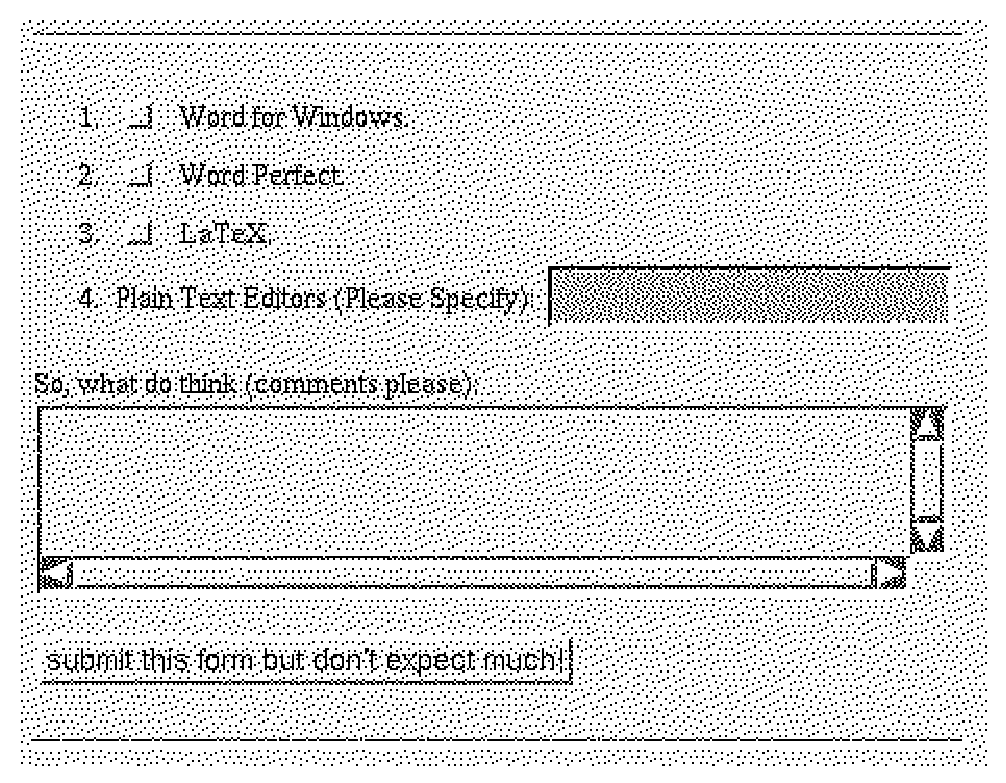
\psfig{file=eform.ps,width=4in}} \\
     Figure: An electronic form. Of course in the online version of this
document the form above would be active.
    \end{center}
\end{figure}
\end{latexonly}

{\bf Warning:} Avoid using LaTeX commands involving counters (e.g.
numbered figures or equations) in conditional text because this may 
disrupt the values of the counters in the electronic version.

% The argument here used to have a \label in its argument which caused
% the ``Contents'' page entry not to be hyperized.
\subsection{Conditional Text}
\label{sec:latexonly}
\index{latexonly} \index{htmlonly}
Conditional text can be specified using the environments {\tt latexonly} and {\tt
htmlonly}. These allow writing parts of a document which are intended
only for electronic delivery or only for paper-based delivery. 

This would be useful for example in adding a long description of a
multimedia resource in the paper version of a document. Such a
description would be redundant in the electronic version, as the user
can have direct access to this resource. 

Here is an example of the use of the {\tt latexonly} environment:

\begin{verbatim}
\begin{latexonly}
\begin{figure}
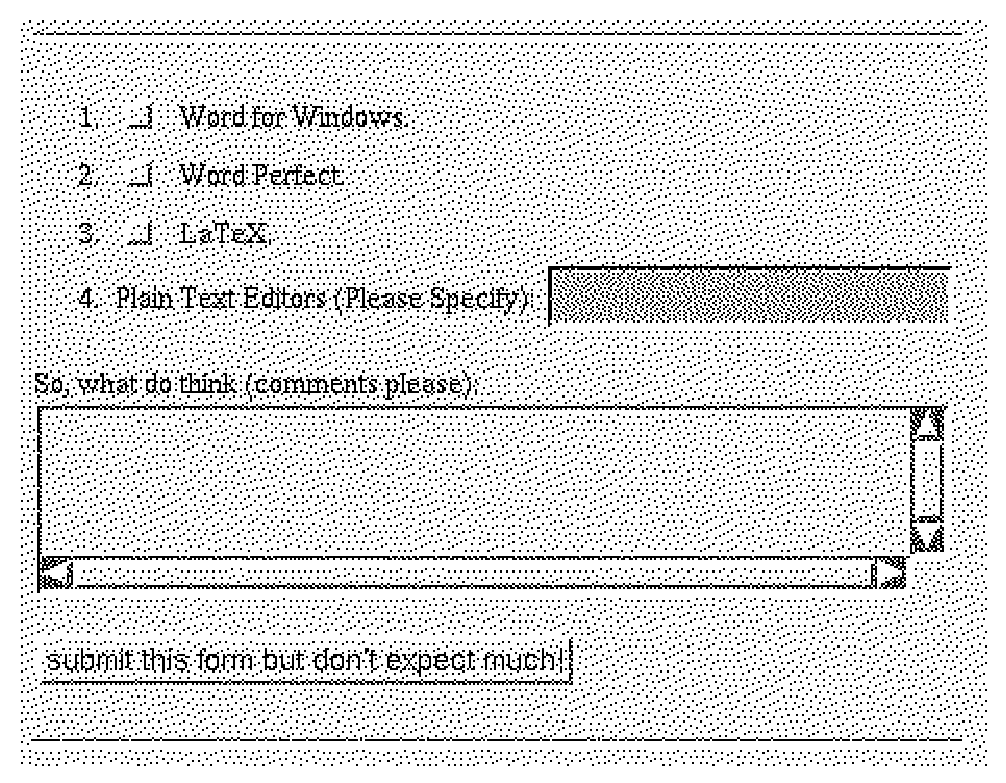
\psfig{file=eform.ps,width=4in}
\caption{An electronic form. Of course in the online version 
of this document the form above would be active!}
\end{figure}
\end{latexonly}
\end{verbatim} 

\subsection{Cross References Shown as ``Hyperized'' Text}

\index{cross-references}
In printed documents cross-references are shown through a {\em numerical
or symbolic indirection} e.g. ``see Figure 1'' (numeric indirection), or
``see section ``Changes'' (symbolic indirection).  \latextohtml can
mirror this mechanism using the same numeric or symbolic references,
or when these are
not appropriate by using iconic references.

In a hypertext document however, cross-references can be shown 
without any indirection just by highlighting a relevant piece of
text. This can make a document more readable as it removes unnecessary
information. 

A single new LaTeX command {\tt hyperref} can be used for
specifying how a cross-reference should appear both in the printed
document and in the hypertext version.

Assuming that the label \verb|sec:cond| is defined somewhere
in a document the command {\tt hyperref} which takes 4 arguments
can be used in the same document as follows:

\index{hyperref} \index{conditional text}
\begin{verbatim}
{\em Is the concept of
\hyperref
% This will be highlighted in the hypertext version
{conditional text}			% argument #1
% This will be shown in the printed version 
% followed by a numeric reference ...      
{conditional text (see Section }  	% argument #2
% ... followed by this text
{ for more information)} 		% argument #3
% This the common label 
{sec:cond}				% argument #4
a good idea? }
\end{verbatim}

Here is how it will be shown: \\
{Is the concept of
\hyperref
% This will be highlighted in the hypertext version
{conditional text}
% This will be shown in the printed version  
% followed by a numeric reference ...      
{conditional text (see Section }  
% ... followed by this text
{ for more information)} 
% This the common label 
{sec:cond}
a good idea? }

\begin{htmlonly}
In the printed version what would appear is: \\
{ Is the concept of conditional text (see Section XXX for more information) a good idea? }
\end{htmlonly}

\begin{latexonly}
In the hypertext version what would appear is:\\
{ Is the concept of \underline{conditional text} a good idea?} \\
Of course \underline{conditional text} would be an active hypertext link.
\end{latexonly}


Another command also defined in {\fn html.sty} is {\tt htmlref} 
which has the same effect as {\tt hyperref} during the conversion to
HTML.
It takes two arguments, some text and a label. In the HTML version the
text will be ``hyperized'' pointing to the label. In the paper version
the text will be shown as it is and the label will be ignored eg

\begin{small}
\begin{verbatim}
With {\tt htmlref} \htmlref{it's easy to make links}{fig:example}.
\end{verbatim}
\end{small}

\begin{htmlonly}
In the HTML version it will be shown as: \\
With {\tt htmlref} \htmlref{it's easy to make links}{fig:example}.
\end{htmlonly}
\begin{latexonly}
In the HTML version it will be shown as: \\
With {\tt htmlref} \underline{it's easy to make links}.
\end{latexonly}


\subsection{Customizing the Navigation Panel}
\index{navigation panel} \label{sec:navpanel}
The navigation panel is the strip containing ``buttons'' and text
that appears at the top
and perhaps at the bottom of each generated page and provides
hypertext
links to other sections of a document. Some of the
options and variables that control whether and where it should appear 
\hyperref{have already been mentioned}{have already been mentioned in 
Section }{}{navoptions}. 


A simple mechanism for appending customized buttons to the navigation
panel is provided by the command {\tt htmladdtonavigation}. This takes
one
argument which \latextohtml appends to the navigation panel. For
example,
\begin{verbatim}
\htmladdtonavigation
   {\htmladdnormallink
      {\htmladdimg{http://server/mybutton.gif}}
      {http://server/link}}
\end{verbatim}
will add an active button {\tt mybutton.gif} pointing to the specified location.


Apart from these facilities it is
also 
possible to specify completely what appears in the navigation panel 
and in what order. As each section is processed, \latextohtml
assigns relevant information to a number of global variables.
These variables are used by the subroutine {\fn navigation$\_$panel}
where the navigation panel is constructed as a string consisting of
these variables and some formatting information. 

This subroutine
can be redefined in a system or a user configuration file ({\fn
LATEX2HTMLDIR/latex2html.config} and {\fn HOME/.latex2html-init} 
respectively). {\em Any combination of text, HTML tags, 
and the variables mentioned below is acceptable}. 

The control panel variables are:

{\bf Iconic links (buttons)}
\begin{itemize}
\item PREVIOUS - points to the previous section 
\item UP  - points up to the "parent" section
\item NEXT - points to the next section
\item NEXT$\_$GROUP - points to the next "group" section
\item PREVIOUS$\_$GROUP - points to the previous "group" section
\item CONTENTS - points to the contents page if there is one
\item INDEX - points to the index page if there is one
\end{itemize}

{\bf Textual links (section titles)}
\begin{itemize}
\item PREVIOUS$\_$TITLE - points to the previous section
\item UP$\_$TITLE  - points up to the "parent" section
\item NEXT$\_$TITLE - points to the next section
\item NEXT$\_$GROUP$\_$TITLE - points to the next "group" section
\item PREVIOUS$\_$GROUP$\_$TITLE - points to the previous "group" section
\end{itemize}

If the corresponding section exists each iconic button will contain an
active link to that section. If the corresponding section does
not exist, the button will be inactive. If the section corresponding
to a textual link does not exist then the link will be empty.

The number of words that appears in each textual link
is controlled by the variable {\fn WORDS$\_$IN$\_$NAVIGATION$\_$PANEL$\_$TITLES}
which may also be changed in the configuration files.

Below is an example of a navigation panel 
(the ``.'' is the Perl string concatenation operator and ``\#''
signifies
a comment).

\begin{small}
\begin{verbatim}
sub navigation_panel {

    #  Start with a horizontal rule (3-d dividing line)
    "<HR> ".			
    
    # Now add few buttons with a space between them
    "$NEXT $UP $PREVIOUS $CONTENTS $INDEX $CUSTOM_BUTTONS" .
	    
    "<BR>\n" .		# Line break
	
    # If ``next'' section exists, add its title to the navigation panel
    ($NEXT_TITLE ? "<B> Next:</B> $NEXT_TITLE\n" : undef) . 
    
\end{verbatim}
\begin{verbatim}
    # Similarly with the ``up'' title ...
    ($UP_TITLE ? "<B>Up:</B> $UP_TITLE\n" : undef) . 
 
    # ... and the ``previous'' title
    ($PREVIOUS_TITLE ? "<B> Previous:</B> $PREVIOUS_TITLE\n" : undef) .
   
    #  Horizontal rule (3-d dividing line) and new paragraph  
    "<HR> <P>\n"		
}
\end{verbatim}
\end{small}

\subsection{Indicating Differences Between Document Versions} 

\latextohtml supports the {\fn changebar.sty} package by David B. Johnson 
(dbj@titan.rice.edu), for 
inserting ``change bars'' in a document in order to indicate 
differences from previous versions. This is a very primitive form of 
version control and there is much scope for improvement.


\subsection{Hypertext Links in Bibliographic References (Citations)}
If a report or a book that is cited (using the {\tt cite}) 
command is available (or there is information about it) on WorldWide
Web then it is possible to add the appropriate hypertext links
in your bibliographic database (the {\fn .bib}) file. 

Here is an example of a bibliographic entry for the original
LaTeX\cite{lamp:latex} book:

\begin{small}
\begin{verbatim}
@book{lamp:latex,
title = "LATEX User's Guide \& Reference Manual",
year = 1986 ,
author = "Leslie Lamport",
Publisher = "Addison-Wesley Publishing Company, Inc.",
note = "Online information on TeX and LaTeX is available at
\htmladdnormallink{http://curia.ucc.ie/info/TeX/menu.html}
{http://curia.ucc.ie/info/TeX/menu.html} and
\htmladdnormallink{http://es-sun2.fernuni-hagen.de/info2html?(latex.info)Top}
{http://es-sun2.fernuni-hagen.de/info2html?(latex.info)Top}"}
\end{verbatim}
\end{small}
No other
modifications are required for this to work - LaTeX and BibTeX 
should work as normal.

For those who use the Harvard style for references
\htmladdnormallinkfoot{there exists a special conversion
add-on package}{http://www.arch.su.edu.au/\~{}peterw/latex/harvard/}.

\subsection{Internationalization}
A special variable {\tt LANGUAGE\_TITLES} 
in the initialization or configuration files determines the language 
in which some section titles will appear. For example setting it to 
\begin{verbatim}
$LANGUAGE_TITLES = ``french'';
\end{verbatim}
will cause LaTeX2HTML to produce ``Table des mati\`{e}res'' instead of
``Table of Contents''.

The only languages currently supported are ``french'' and ``english''
but it is trivial to add support for another language in the
file {\fn latex2html.config}. As a guide here is the entry for 
the French titles:
\begin{verbatim}
sub french_titles {
 $toc_title = "Table des mati\\`eres";	
 $lof_title = "Liste des figures";
 $lot_title = "Liste des tableaux";
 $idx_title = "Index";
 $bib_title = "R\\'ef\\'erences";		
 $info_title = "\\`A propos de ce document..."; 
}
\end{verbatim}

In order to provide full support for another language you may also
want to replace the navigation buttons which come with \latextohtml 
(which are by default in
English)
with your own. As long as the new buttons have the same filenames as the
old ones there should not be a problem.

\subsection{Image Conversion}
\label{imgcon}

\latextohtml converts equations, special accents, external postscript
files, and LaTeX environments it cannot directly translate into 
inlined images. This section describes how it is possible to control
the final appearance of such images. For the purposes of the discussion below,

\begin{description}
\item[{\bf ``small images''}] will refer to equations, special accents and
any other image generating LaTeX commands, while 
\item[{\bf ``figures''}] will
apply  to any image generating LaTeX environments (eg figure, table,
minipage etc).
\end{description}

The size of all ``small images'' depends on a configuration variable
{\tt MATH\_SCALE\_FACTOR} which specifies how much to enlarge or 
reduce them in relation to their original size in the postscript 
version of the document. For example a scale factor of 0.5 will make all 
images half as big while a scale factor of 2 will make them twice as
big.
Larger scale factors result in longer processing times and larger 
intermediate image files. A scale factor will only be effective 
if it is greater than 0. 

The configuration variable {\tt FIGURE\_SCALE\_FACTOR} performs
a similar function for ``figures''. Both of these configuration 
variables are initially set to 1.6.

For finer control, several
parameters affecting the conversion of a single ``figure'' 
can be controlled
with the command {\tt htmlimage} which is defined in {\fn
html.sty}.
The one argument of {\tt htmlimage}
is a string of options separated by commas. The options are
\begin{verbatim}
scale = <scale factor>
external
thumbnail = <scale factor>
map = <image map URL>
\end{verbatim}

The {\tt scale} option allows control over the size of the final
image.

The {\tt external} option will cause the image not to be inlined 
(images are inlined by default). External images will be accessible
via a hypertext link. 

The {\tt thumbnail} option will cause a small inlined image to be 
placed in the caption. The size of the thumbnail depends on the
scale factor. The use of the {\tt thumbnail} option implies
the {\tt external} option. In order to be effective the command
{\tt htmlimage} and its options {\bf must be placed inside the
environment on which it will operate}.

The {\tt map} option will turn the inlined image into an 
\htmladdnormallink{active
image map}{http://wintermute.ncsa.uiuc.edu:8080/map-tutorial/image-maps.html}.

{\bf Example:}
The effect of the LaTeX commands below can be seen in the
\htmlref{thumbnail sketch of Figure}{fig:example} \ref{fig:example}.
\begin{small}
\begin{verbatim}
{\begin{figure}[tbh]
    \htmlimage{thumbnail=0.5}
    \centerline{
    \psfig{file=figure.ps,width=5in}}
    \caption{A sample figure showing part of a page generated by
\latextohtml containing a customized navigation panel (from the
\protect\htmladdnormallinkfoot{CSEP project}
{http://csep1.phy.ornl.gov/csep.html}).}
    \label{fig:example}
\end{figure}}
\end{verbatim}
\end{small}

The {\tt htmlimage} command is also often useful to cancel-out the
effect of the configuration variable {\tt FIGURE\_SCALE\_FACTOR}.
For example to avoid resizing a color screen snap despite 
the value of {\tt FIGURE\_SCALE\_FACTOR} it is possible to 
use {\tt htmlimage\{scale=0\}}.

\subsection{Figures, Tables and Arbitrary Environments}
\index{figures} These are here to show how the translator
handles figures, tables
and other environments. Compare the paper with the online version.

\index{tables}
\begin{table}[h]
\begin{center}
\begin{tabular}{||l|lr||}   \hline
gnats	&	gram	&	\$13.65  \\ \cline{2-3}
	&	each	&        .01	\\ \hline
gnu	& 	stuffed	&        92.50  
                \\  \cline{1-1} \cline{3-3}
emur	&		&	33.33   \\ \hline
armadillo	& frozen	&	8.99 \\ \hline
\end{tabular}
\end{center}
\caption{A sample table taken from \protect\cite{lamp:latex}}
\label{tab}
\end{table}

\index{numbered equations}
Here are some some automatically numbered right-justified equations
\begin{equation} 
\Phi_{l+1,m,n} = (\Phi+h\frac{\partial\Phi}{\partial x} +
\frac{1}{2}h^2\frac{\partial^2\Phi}{\partial x^2} +
\frac{1}{6}h^3\frac{\partial^3\Phi}{\partial x^3} + \ldots)_{l,m,n}
\end{equation}
with some gratuitously \'{a}cc\"{e}nted text in between them.
\begin{eqnarray}  \label{eq:demo}
\frac{\Phi_{l+1,m,n}-2\Phi_{l,m,n}+\Phi_{l-1,m,n}}{h^{2}} +
\frac{\Phi_{l,m+1,n}-2\Phi_{l,m,n}+\Phi_{l,m-1,n}}{h^{2}} + \nonumber \\
\frac{\Phi_{l,m,n+1}-2\Phi_{l,m,n}+\Phi_{l,m,n-1}}{h^{2}} = -I_{l,m,n}(v)
\end{eqnarray}

{\begin{figure}[tbh]
    \htmlimage{thumbnail=0.5}
    \centerline{
    \psfig{file=figure.ps,width=5in}}
    \caption{A sample figure showing part of a page generated by
\latextohtml containing a customized navigation panel (from the
\protect\htmladdnormallinkfoot{CSEP project}
{http://csep1.phy.ornl.gov/csep.html}).}
    \label{fig:example}
\end{figure}}

\section{Getting LaTeX2HTML}
\index{source code}
\begin{flushleft}
The \htmladdnormallink{source code can be obtained 
at http://cbl.leeds.ac.uk/nikos/tex2html/latex2html.tar.}
{http://cbl.leeds.ac.uk/nikos/tex2html/latex2html.tar}
or \htmladdnormallink{as a compressed archive at http://cbl.leeds.ac.uk/nikos/tex2html/latex2html.tar-gz}{http://cbl.leeds.ac.uk/nikos/tex2html/latex2html.tar-gz}
The source code is also available 
via anonymous FTP at 
\htmladdnormallink{ftp://ftp.tex.ac.uk/pub/archive/support/latex2html}{ftp://ftp.tex.ac.uk/pub/archive/support/latex2html}
or
\htmladdnormallink{ftp://sunsite.unc.edu/pub/packages/infosystems/WWW/tools/translators/latex2html}{ftp://sunsite.unc.edu/pub/packages/infosystems/WWW/tools/translators/latex2html}.
Other FTP sites nearer to you can be found using {\fn Archie}
at
\htmladdnormallink{http://hoohoo.ncsa.uiuc.edu/archie.html}{http://hoohoo.ncsa.uiuc.edu/archie.html}
or 
\htmladdnormallink{http://www.pvv.unit.no/archie/}{http://www.pvv.unit.no/archie/}
(faster).

{\bf Warning:} Some FTP sites may not carry the latest version.

Updates and patches are posted on the \latextohtml server at
\htmladdnormallink{http://cbl.leeds.ac.uk/nikos/tex2html/doc/latex2html/latex2html.html}{http://cbl.leeds.ac.uk/nikos/tex2html/doc/latex2html/latex2html.html}

\end{flushleft}

If you get the {\tt tar} version, save it into a file, say {\tt latex2html.tar}
and then extract the files with 
\begin{verbatim}
% tar xvf latex2html.tar
\end{verbatim} 

You should then have the following:
\begin{itemize}
\item A {\fn README} file.
\item A {\fn Changes} file.
\item The {\fn latex2html} Perl program.
\item A \index{texexpand} {\fn texexpand} Perl program \footnote{Written 
by Robert S. Thau $<$rst@edu.mit.ai$>$.}.
\item A {\fn latex2html.config} configuration file.
\item An {\fn install-test} installation and testing Perl script.
\item A {\fn dot.latex2html-init} sample initialization file.
\item A {\fn html.sty} style file.
\item A {\fn pstogif} perl script.
\item Two {\fn pstoppm.ps} files.
\item A {\fn docs/} subdirectory containing a version of this
manual.
\item An {\fn icons/} subdirectory containing various icons.
\item A {\fn styles/} subdirectory containing Perl code for handling
some style files.
\end{itemize}
\section{Requirements}
\index{requirements}
The translator makes use of several utilities all of which 
are freely available on most platforms. \htmladdnormallinkfoot{You may use 
{\fn Archie} to find the source code of any utilities you might need.}
{http://www.pvv.unit.no/archie/}

The requirements for using \latextohtml 
depend on the kind of translation you would like to perform, as follows:

\begin{enumerate}
\item {\bf LaTeX commands but without equations, figures, tables, etc.} \hfill
\begin{itemize}
\item \htmladdnormallink{{\fn Perl}}{ftp://ftp.uu.net/languages/perl/} 
(version 4.0 - RCSfile: perl.c,v - Revision: 4.0.1.8 - Date:
1993/02/05 19:39:30 - Patch level: 36)

{\bf Warning:} You really DO need Perl at patch level 36 or later.
Versions of \latextohtml earlier than 0.7a4 work {\bf only} with 
Perl 4 at patch level 36. Later versions of \latextohtml work 
both with Perl 4 at patch level 36 and Perl 5. {\bf No} version 
of \latextohtml will work  with Perl 4 at earlier patch levels.

\item {\fn DBM} or {\fn NDBM}, the Unix DataBase Management system.
\end{itemize}

\item {\bf LaTeX commands with equations, figures, tables, etc.} \\
As above plus
\begin{itemize}
\item {\fn latex},
\item  \htmladdnormallink{{\fn dvips}}
{ftp://ftp.tex.ac.uk/pub/archive/dviware/dvips}
(version  5.516 or later) or {\fn dvipsk}.
\item {\fn gs} (Ghostscript version 2.6.1 or later). 
\item The \htmladdnormallink{{\fn
pbmplus}}{ftp://ftp.x.org/R5contrib/}
OR \htmladdnormallink{{\fn
netpbm}}{ftp://ftp.x.org/R5contrib/}
library.
Some of the filters in those libraries are used during the postscript to
GIF conversion. 
\end{itemize}

\item 
{\bf \htmladdnormallinkfoot{Transparent inlined images}{http://melmac.corp.harris.com/transparent\_images.html}}\\
If you dislike the ugly white background color of the
generated inlined images then you should get either 
the {\fn netpbm} library (instead of the older {\fn pbmplus}) OR
install the
\htmladdnormallinkfoot{{\fn
giftrans}}{ftp://ftp.rz.uni-karlsruhe.de/pub/net/www/tools/giftrans.c}
filter by Andreas Ley $<$ley@rz.uni-karlsruhe.de$>$. 
Version 1.10.2 is
known to work without problems but later versions should also be OK.

\end{enumerate} 

If {\fn ghostscript} or the {\fn pbmplus} (or {\fn netpbm}) library are not
available it
is still possible to
use the translator with the {\tt -no\_images} option. 

If you intend to use any of the special features of the translator (see Page \pageref{special})
then you have to include the 
{\fn html.sty} file in any LaTeX documents that use them. 

Because by default the translator makes use of inlined images in the final 
HTML output, it would be better to have a viewer which supports 
the {\tt $<$IMG$>$} tag, such as \htmladdnormallink{NCSA 
Mosaic}{http://www.ncsa.uiuc.edu/SDG/Software/Mosaic/Docs/help-about.html}.
If only a character based browser is available or if you want the
generated
documents to be more portable then the translator can be used
with the 
\hyperref{{\tt -ascii$\_$mode} option}{{\tt -ascii$\_$mode} option (See
Section }{ )}{asciimode}. 

\section{Installing LaTeX2HTML}

To install \latextohtml you {\bf MUST} do the following:

\begin{enumerate}
\item {\bf Specify where Perl is on your system}. \\
In each of the files {\fn latex2html}, {\fn texexpand} {\fn pstogif}
and  {\fn install-test},
modify the first line saying where Perl is on your system. 

Some system administrators do not allow Perl programs to run as shell
scripts. This means that you may not be able to run any of the above
programs. {\em In this case change the first line in each of these
programs from}
\begin{verbatim}
#!/usr/local/bin/perl
\end{verbatim}

{\em to}

\begin{verbatim}
: # *-*-perl-*-*
    eval 'exec perl -S  $0 "$@"'
    if $running_under_some_shell; 
\end{verbatim}

\item {\bf Specify where the external utilities are on your system.} \\
In the file {\fn latex2html.config} give the correct pathnames for 
some directories (the {\fn latex2html} directory and the {\fn 
pbmplus} or {\fn netpbm} library) and some executables ({\fn latex, dvips, gs}). 
Note that it is
possible 
to use \latextohtml even
if you don't have some of the external utilities.

While you're at it you may want to change some of the default 
options in the same file.

\item {\bf Run {\fn install-test}.} \\
This Perl script will make some changes in the {\fn latex2html} file
and then check whether the pathnames to any external utilities
(specified during the previous step) are correct. It will not actually
install the external utilities. 

Don't forget to make {\fn
install-test} executable (using the {\fn chmod} command) before
using it if necessary. You may also need to make the files
{\fn pstogif}, {\fn texexpand} and {\fn latex2html} executable 
if {\fn install-test} fails to do it for you.

If for any reason you have trouble running {\fn install-test}
do not despair. Most of what it does is to do with checking
your installation rather than actually installing anything.
To do a {\bf manual installation} just change the variable
{\tt LATEX2HTMLDIR} in the beginning of the file {\fn latex2html}
to point to the directory where the \latextohtml files can be found.
\end{enumerate}

This is enough for the main installation but you may also 
want to do some of the following:
\begin{itemize}

\item {\bf To use the new LaTeX commands which are defined in {\fn html.sty}:} \\
Make sure that LaTeX knows where the html.sty
file is, either by putting it in the same place as the other style files on
your system, or by changing your TEXINPUTS shell environment variable,
or by copying html.sty in the same directory as your LaTeX source file.

\item {\bf To set up different initialisation files:} \\
For a ``per user'' initialisation file, 
copy the file {\fn dot.latex2html-init} in the home directory
of any user that wants it, modify it according to her preferences and
rename it as {\fn .latex2html-init}. At runtime, both the {\fn 
latex2html.config} file and {\fn \$HOME/.latex2html-init} file will be
loaded, but the latter will take precedence.

You can also set up a ``per directory'' initialisation file by 
copying a version of {\fn .latex2html-init} in each directory you
would like it to be effective. An initialisation file
{\fn /X/Y/Z/.latex2html-init} will take precedence over all other
initialisation files if {\fn /X/Y/Z} is the ``current directory'' when
\latextohtml is invoked.

\item {\bf To make your own local copies of the \latextohtml icons:} \\
Please copy the {\fn icons} subdirectory to a 
place under your WWW tree
where they can be served by your server.
Then modify the value of the {\fn \$ICONSERVER} variable in 
{\fn latex2html.config} accordingly. 

{\bf Warning:} If you cannot do that
bear in mind that these icons will have
to travel from Leeds!!! Also, your documents will depend on our
server being operational in the first place.

\item  {\bf To make your own local copy of the \latextohtml
documentation:} \\
This will also be a good test of your installation. 
To do it run \latextohtml on the file {\fn docs/manual.tex}.
You will get better results if you run LaTeX first on the 
same file in order to create some auxiliary files.

\item {\bf To join the community of \latextohtml users:} \\
More information on a mailing list, discussion archives, bug reporting
forms and more is available at \\
\htmladdnormallink{http://cbl.leeds.ac.uk/nikos/tex2html/doc/latex2html/latex2html.html}
{http://cbl.leeds.ac.uk/nikos/tex2html/doc/latex2html/latex2html.html}
\end{itemize}

\section{Changes from Previous Versions}
The \htmladdnormallink{previous versions of the
translator and some patches}{http://cbl.leeds.ac.uk/nikos/tex2html/previous-versions}
are available. A \htmladdnormallink{detailed list of changes}
{http://cbl.leeds.ac.uk/nikos/tex2html/doc/Changes.txt}
which includes full credits to all who have contributed 
bug fixes or other code is also available with the
\latextohtml distribution in the file {\fn Changes}.


\subsection{Changes upto v95}
\begin{description}
\item[{\bf Much improved inlined equation baseline alignment!}]
(Thanks to Mark Segal $<$segal@spud.asd.sgi.com$>$)
Inlined equation bitmaps are now aligned correctly depending 
on whether they contain subscripts, superscripts etc. 
\item[{\bf Support for internationalization}]
(Thanks to Martin Boyer $<$gamin@ireq-robot.hydro.qc.ca$>$)
A global variable {\tt LANGUAGE\_TITLES} can now be used to change the
language in which some section titles (eg ``Table of Contents'') are
printed. It is also very easy to add support for more languages.
\item[{\bf Compatibility with Perl 5}]
\item[{\bf More efficient implementation}]
There has been a major overhaul of the way the source text is parsed
and analysed in order to reduce the memory requirements of this
process.

This has been achieved by spawning off separate Unix processes to deal
with each of the {\tt input}'ed or {\tt include}'d files. As each
process
terminates all the space that it used is reclaimed. 
Asynchronous communication between processes takes place using 
the Unix DataBase Management system (DBM or NDBM) 
which should be present
on your system.

{\bf To take advantage of these changes}, 
it is necessary to split the source text 
into more than one files which can be assembled using the \LaTeX
{\tt input} or {\tt include} commands.


\item[{\bf ``Off-line'' Image Generation}]

Two new options {\tt -no\_images} and {\tt  -images\_only} allow
``off-line'' image conversion. The advantage of using these options is 
that the translation can be allowed to finish even when there are
problems with image conversion. In addition it may be possible to 
fix manually any image conversion problems and then run \latextohtml 
again just to integrate the new images without having to translate
the rest of the text. More instructions on how to do this are
included in the ``Troubleshooting'' section of the \latextohtml
manual.

Can now use either the {\fn pbmplus} or the {\fn netpbm} libary.
If {\fn netpbm} is used then it is no longer necessary to get and
install {\fn giftrans} in order to generate transparent inlined 
images.

Also, a new option {\tt map=$<$image map URL$>$} in the 
command {\tt htmlimage} can turn an included postscript image into an active
image map.

\item[{\bf New options}] \hfill
\begin{description}
\item [-no\_images]
Do not attempt to produce any inlined images. 
The missing images can be generated "off-line" by restarting \latextohtml
with the option {\tt -images\_only}.
\item [-images\_only]
Try and convert any inlined images that were left over from previous
runs of \latextohtml. 
\item [-no\_reuse]
Do {\bf not} reuse images generated during previous translations.
(This will enable the initial interactive session during which the user is
asked whether to reuse the old directory, delete its contents or quit)
\item [-no\_subdir]
Place the generated HTML files  in the 
current directory. The default behaviour is to create (or reuse)
another file directory.
\item [-ps\_images]
Use links to external postscript images rather than inlined GIF images.
\end{description}
\item[{\bf Several small changes and bug fixes}] \hfill
\begin{itemize}
\item It is no longer necessary to get {\fn Giftrans} if {\fn NETPBM}
is available
\item Fixed problems with support for {\fn german.sty}
\item Fixed problems with multiple bibliographies. Each bibliography
is now treated as a separate section.
\item Added support for ``dotless i's and j's''.
\item  Fixed to resolve figure and table numbers when captions contain
accented characters.
\item Added support for hierarchical indices with duplicate index keys
\item Fixed problem with HTML encodings of ISO-LATIN1 characters   
creeping into converted images of figures and tables.
\item  Added new global variable {\tt PAPERSIZE}
to make it easier to change the default behavior when converting large images
\item A new configuration variable ({\tt TRANSPARENT\_IMAGES}) can be 
used to stop any inlined images generated from "figure" environments
from being transparent.
\item Fixed problem which occurs when {\fn getcwd.pl} is not part of the
Perl library.
\item The option {\tt -address ""} is now valid.
\item Fixed a problem with tables of contents.
\item Fixed problem with the use of the {\tt finger} command when
trying to find out the name of the user.
\item Added some support for {\tt tabbing} environments.
\item HTML heading elements no longer contain other markup.
\item Fixed problem with optional argument in citation commands
\item Added some more support for LaTeX2e.
\item Fixed problem with displayed equations forcing all the remaining
equations to be displayed.
\item Fixed bug with converting postscript images containing more than
256 colors.
\end{itemize}
\end{description}

\subsection{Changes upto v0.6.2}

\begin{description}
\item[{\bf Image Conversion}] \hfill
\begin{itemize}
\item The {\fn pstogif} script has been rewritten in Perl and it
now accepts more options for specifying color depth, scale factors
and pixel density.
\item LaTeX {\tt figure} and other environments are now processed
in 24-bit color.
\item Figure and table captions are now converted into HTML
rather than becoming part of the inlined image. This means that 
any cross-references in the captions will become active.
\item It is now possible to control for each generated image:
\begin{itemize}
\item its size 
\item whether it should be inlined or left as an external image
\item if left as an external image whether it should be accessible
via a \htmlref{{\bf generated thumbnail sketch}}{fig:example}
or a textual hypertext link
\end{itemize}
These options are available from a new LaTeX command defined in {\fn
html.sty} called {\fn htmlimage}. 

\item Equations and other inlined images are converted into
transparent GIFs rather than XBMs. {\bf This makes it possible 
to reduced their storage requirements to about 1/6th of what was
previously required!}
\item The default size of equations and other small inlined 
images can be changed
by setting the variable {\tt MATH\_SCALE\_FACTOR} in the
configuration files.
\item The default size of figures, tables, and other large
inlined images can be changed by setting the variable 
{\tt FIGURE\_SCALE\_FACTOR} in the
configuration files.

\item Dvips is now called with the {\tt -M} option which stops it
from invoking {\tt METAFONT}.
\end{itemize}

\item[{\bf Optimization}] \hfill
\begin{itemize}
\item Some effort has gone into reducing the amount of memory required
during conversion. {\bf The impact of these changes can be very
significant}.
In particular, files
containing large numbers of LaTeX commands (eg {\fn .aux} or {\tt .bib}) 
files are handled much better.
\end{itemize}

\item[{\bf Backwards Incompatible Changes}] \hfill
\begin{itemize}
\item The option {\tt -allbitmaps} has been removed. This is no
longer necessary as \latextohtml can now generate transparent
GIF images.
\item The definition of the command {\tt htmladdnormallink} in the 
file {\fn html.sty} has changed and the URL will no longer appear
as a footnote in the paper (DVI) version. The translation of
this command into HTML is {\bf not} affected. 

The previous functionality can be obtained with a new command
{\tt htmladdnormallinkfoot} which will add the URL as a footnote
in the paper version.
\item The script {\fn pstoxbm} is no longer distributed as it is not
used.

\end{itemize}

\item[{\bf Bug Fixes}] \hfill
\begin{itemize}
\item The {\fn install-test} script now recognizes version
numbers correctly and gives better warnings. It also makes
executable any scripts that need to be so. 
\item Stopped using the {\tt nslookup} program to try and guess
e-mail addresses (they were used in signing each generated page). 
This has been replaced with a simple call 
to {\tt finger}.
\item Fixed problem which could cause ``Parameter overflow'' in 
TeX during image conversion.
\item The {\fn texexpand} script has been changed extensively.
Some nasty looping problems are now avoided, and the tracking
down of included files has been improved.
\item Some reported incompatibilities with some Unix shells
(bash,OSF) have been fixed.
\item Displayed equations now appear correctly on separate
lines and are right justified.
\item Fixed bug with nested environments.
\item Fixed problem which caused the wrong numbers to be assigned
to sections with the same titles when the {\tt -show\_section\_titles}
is used (thanks to Brian  Toonen $<$toonen@mcs.anl.gov$>$).
\item Fixed problem with the {\tt hyperref} command which
caused the wrong ``hyperized'' text to appear in the final document.
\item {\tt item} optional arguments can now contain one level of
nesting eg {\tt item[[First Choice]]}.
\item Fixed problems with the ``image caching and reuse'' mechanism 
which avoids converting images unnecessarily..
\end{itemize}

\item[{\bf Other Changes}] \hfill
\begin{itemize}
\item LaTeX2HTML now generates $<$meta$>$ HTML tags which can be used
by \htmladdnormallinkfoot{indexing scripts}
{http://www.ai.mit.edu/tools/site-index.html}
 which generate information for the \htmladdnormallinkfoot{ALIWEB}
{http://web.nexor.co.uk/aliweb/bin/aliwebsimple.pl} 
search and retrieval tool. The information in the $<$meta$>$ tags
contains
the title of each separate HTML file. 
\item A new configuration variable {\tt DEBUG} can be used to preserve
intermediate files for debugging. 
\item Some problems with respect to compatibility with the HTML2.0 
standard have been addressed. No more ``unquoted attribute value literals''.
\item All the navigation icons are now ``lynx friendly''; their
{\tt ALT} attribute now has a meaningful value.
\item A new LaTeX command {\fn htmlref} makes it a lot simpler
to create hypertext links intended only for the HTML version of
the document.
\item {\fn DVIPSK} is now recognized by the installation script
\item Added support for the {\fn changebar.sty} file by 
David B. Johnson (dbj@titan.rice.edu).
\item It is no longer necessary to add style file names into the 
{\tt DONT\_INCLUDE} variable as \latextohtml now does not
attempt to translate file included files ending in {\tt .sty}.
\item The small invisible bitmaps that used to mark anchors have been
replaced with the invisible character \verb|&#160;|.
\item It is no longer necessary to use full pathnames when
including external postscript files.
\item If a file {\fn .latex2html-init} is found in the ``current
directory'' then this will be loaded automatically after loading the
other default configuration files.
\item Changed the naming convention of generated HTML files. The
``top'' document is {\fn $<$FILE$>$.html} as before but all other ``nodes''
are named {\fn nodeN.html} where {\fn N} is an integer. Also, the file
containing
the footnotes is now called {\fn footnode.html}.
\item A special extension to \latextohtml for those who use the 
Harvard style for references can be obtained from
\htmladdnormallink{http://www.arch.su.edu.au/\~{}peterw/latex/harvard/}{http://www.arch.su.edu.au/\~{}peterw/latex/harvard/}.
\end{itemize}
\end{description}


\subsection{Changes upto v0.5.3}
\begin{itemize}
\item The files {\fn LATEX2HTMLDIR/styles/german.perl} and 
{\fn LATEX2HTMLDIR/styles/makeidx.perl} have been fixed
so that they are consistent with changes in the main script.
\item A problem with disappearing spaces after some equations
and other environments has been fixed.
\end{itemize}
\subsection{Changes upto v0.5.1}
\begin{description}
\item[{\bf Navigation Panel}]
The \hyperref{navigation panel}{navigation panel (see section
}{)}{sec:navpanel}
is now fully configurable and much better looking.
\item[{\bf Automatic Signatures}]
The signatures at the bottom of each page are now constructed
using {\fn nslookup} (Thanks to Alberto Accomazzi
$<$alberto@cfa.harvard.edu$>$)
\item[{\bf Numerous fixes including...}] \hfill
\begin{itemize}
\item ``dead'' {\fn next$\_$page} buttons when the {\fn -split} option
was used, and
\item internal \latextohtml markers appearing in section titles.
\end{itemize}
\end{description}

\subsection{Changes upto v0.4}
\begin{description}
\item[{\bf Accents and Special Characters}]
LaTeX accent commands, special characters and accent commands defined
in {\fn german.sty} are translated to equivalent ISO-LATIN-1
characters when that is possible (partly thanks to code supplied
by Franz Vojik $<$vojik@de.tu-muenchen.informatik$>$).
\item[{\bf Auto-loading of Style-Specific Code}]
The translator now supports a 
\hyperref{mechanism for including Perl code extensions}{mechanism for
including Perl code extensions (see Section }{)}{sec:sty}
which are specific to particular style files. 


This mechanism will help to keep the core script smaller as well as make
it easier for others to contribute and share solutions on  
how to translate specific style files. The current distribution includes the files
{\fn german.perl}, {\fn french.perl}, {\fn html.perl} and {\fn makeidx.perl}.
\item[{\bf Installation and Testing}]
To make it easier to install the translator for more than one user
there is now a configuration file ({\fn
LATEX2HTMLDIR/latex2html.config}) which contains installation specific 
information and default values for the various options. 
This makes it unnecessary to have a {\fn HOME/.latex2html-init} for
each user.
If a user does have a  {\fn HOME/.latex2html-init} then this will be
loaded after {\fn
LATEX2HTMLDIR/latex2html.config}.

A new Perl script ({\fn install-test}) is now available with the distribution
which will install the translator, and then perform some tests on the
availability
of some external
programs giving, appropriate warnings.
\item[{\bf Navigation Panel Extensions}]
The following new links have been added to the navigation panel which
appears in each page
(where this is appropriate):
\begin{itemize}
\item a link to the next ``logical'' page (this allows reading each
page in the same order as with a paper-based version - as opposed to
structure navigation)
\item a link to the previous ``logical'' page 
\item a link to the table of contents
\item a link to the index 
\end{itemize}
\item[{\bf HTML Style File Extensions}]
The HTML style file {\fn html.sty} now includes definitions of new 
environments for:
\begin{description}
\item[Inclusion of Raw HTML]
A new LaTeX environment {\tt rawhtml} allows
arbitrary
HTML tags to be included in a LaTeX document. This is useful for
taking
advantage of HTML+ features as they become available (e.g. interactive
forms).
The HTML commands are ignored when producing the DVI version of the
document.
\label{sec:cond}
\item[Conditional Text]
The new environments {\tt latexonly} and {\tt htmlonly} allow their
contents to appear only in final DVI or in the HTML version of a
document respectively. 

A new command {\tt hyperref} can be used to specify the way in
which cross-references should be shown in the DVI version and the
HTML version of the document.
\end{description}
\item[{\bf Right Justification of Equations}]
The translator
adds enough whitespace at the beginning of each equation bitmap
to push it to the right-hand margin. The width of each line can be
set in the configuration file using the variable {\tt LINE$\_$WIDTH}.
\item[{\bf Inlined Images}]
All inlined images are now generated by calling {\tt latex} and {\fn
dvips} only once
at the end of the conversion process (but each generated image still
has to be filtered individually). Also, a warning is given if an 
image cannot be converted.
\item[{\bf Numeric Labels}]
The original (LaTeX generated) numeric labels are used instead of
the arrow navigation icon for cross-references where possible.
To do this the translator uses the information in the 
{\fn aux} file which is generated by \LaTeX. If the {\fn aux} file
is out of date a warning is given.
\item[{\bf New Options}] \hfill
\begin{description}
\item[{\tt -auto$\_$navigation}]
This puts a navigation panel 
at the top of each page as usual. But if the page exceeds a
user-settable  
number of words (the default is 450 words) 
then a navigation panel is also placed at the end of
the page. This option is active by default.
\item[{\tt -index$\_$in$\_$navigation}]
Adds a link to the index in the navigation panel.
\item[{\tt -contents$\_$in$\_$navigation}]
Adds a link to the table of contents in the navigation panel.
\item[{\tt -next$\_$page$\_$in$\_$navigation}]
Adds a link to the next ``logical'' page in the navigation panel.
\item[{\tt -previous$\_$page$\_$in$\_$navigation}]
Adds a link to the previous ``logical'' page in the navigation panel.
\item[{\tt -bottom$\_$navigation}]
This puts a navigation panel at the bottom of each page.
\item[{\tt -top$\_$navigation}]
This puts a navigation panel at the top of each page (the default).
\item[{\tt -show$\_$section$\_$numbers}]
This allows each section (page) title to be numbered in the same 
way that it would be numbered by \LaTeX. This requires 
an up to date {\fn aux} file (generated by running \LaTeX) and that 
each title is unique. If the {\fn aux} file is not up to date then a 
warning is given.
Unfortunately if 
the title contains inlined images the numbering for that title will
be lost. 
\item[{\tt -reuse}]
This allows images generated during previous invocations of
the translator to be ``reused'' without going through the initial 
interactive session. The same behavior is obtained by setting
the variable {\tt REUSE} to 1 (the default) in the configuration file.
Note that images which may depend on contextual information (e.g. numerical
labels) cannot be reused and are always re-generated. 
\end{description}
\item[{\bf Bug Fixes and Minor Changes}] \hfill
\begin{itemize}
\item The links from the table of contents in single page documents (created using
the option {\tt -split 0}) is now working as expected.
\item Newlines are translated to the $<$BR$>$ tag.
\item Fixed some problems in dealing with new command macros.
\item {\fn texexpand} now respects commented {\tt input} and {\tt
include} commands. Also (thanks to Franz Vojik
$<$vojik@de.tu-muenchen.informatik$>$), it 
now looks in subdirectories when expanding
files.
\item The ALIGN attribute of inlined images is now BOTTOM instead of
TOP.
\item Fixed problem with the environment variable {\tt TEXINPUTS}.
\item Added some support for optional user-defined labels (bullets) in
list environments.
\end{itemize}
\end{description}

More details on all the changes are available in the file 
{\fn LATEX2HTMLDIR/Changes}.

\subsection{Changes upto v0.3.1}
These changes are mostly due to patches contributed by Robert S. Thau
$<$rst@ai.mit.edu$>$:
\begin{itemize}
\item Nested environments with the same name are now dealt with
properly.
\item Commands that are passed to LaTeX for processing which have 
environments in their arguments (e.g. a {\tt parbox} command which 
an {\tt itemize} environment as an argument) are now
processed correctly. A general mechanism for users to 
specify the syntax of commands that should be passed to LaTeX 
is described in Page \pageref{pass}.
\item Fixed a problem with recognizing the {\tt special} command.
\item Fixed bug in the generation of the index.
\end{itemize}

\subsection{Changes upto v0.3}
\begin{description}
\item [{\bf Image Recycling}]
Images for equations, tables, figures, special characters etc. generated by
the translator are recognised  during subsequent runs.
The user is then asked whether old images should be reused
(or whether the old images should be deleted and regenerated).
This offers tremendous improvements in speed after an initial
successful translation.

\item [{\bf Cross-References Between (Local or Remote) Documents}]
Cross-references between 
two or more documents (possibly on remote locations) can be
established via symbolic labels
which are independent of the physical realisation of these documents. 

Such cross-references will be maintained with a simple
re-translation\footnote{This is true for documents under the same
server but for remote documents a little more is required (see 
the \hyperref{example}{example in Section}{}{crossrefs})}
even after one or more of the documents have been broken into
different physical parts or moved.

The mechanism is based on the 
\hyperref{new commands}{new commands (see Section }{ )}{external}
{\tt externallabels} and {\tt externalref} which are an extension of the simple 
{\tt label-ref} pairs. 

\item [{\bf New Options}] \hfill
\begin{description}
\item [{\tt external$\_$images}] This provides hypertext links to where
generated images (for equations, tables, figures etc) are stored
externally. (The default is to ``inline'' generated images in the main body 
of the text.)
\item [{\tt ascii$\_$mode}] This switches all the navigation icons to their
ascii equivalents. Also generated images are stored externally as with the 
{\tt external$\_$images} option above. The {\tt ascii$\_$mode} option
makes documents more portable as it allows them to be
viewed on browsers that do not support inlined images.
\end{description}
\item [{\bf Special Command Style File}] A style file \htmladdnormallink{{\fn html.sty}} 
{http://cbl.leeds.ac.uk/nikos/tex2html/doc/html.sty.txt} is now included in the
distribution. This contains the definitions (syntax) of some 
special LaTeX commands mainly for providing external hypertext
links.
This should be included in LaTeX files that use the any 
\hyperref{hypermedia extensions}{hypermedia extensions (see Section}{ )}{special}.

\item [{\bf Minor Changes and Bug Fixes}] \hfill
\begin{itemize}
\item Equations, equation arrays and theorems are now numbered
correctly even when they are individually passed to LaTeX for
processing.
\item Fixed problem with {\tt label} commands appearing in section
headings.
\item Fixed problems with verbatim environments, bibliography items,
generated file names, the options {\tt nolatex} and {\tt
no$\_$navigation}, the {\tt thanks command}, the name of an HTML tag
($<$HEAD$>$), 
\item The appearance of footnotes has been improved.
\item Some inconsistencies in the {\fn pstoxbm} and {\fn pstogif}
 scripts have been fixed.  
\item Parts of the documentation have been rewritten, restructured and
some new sections have been added. 
\end{itemize}
\end{description}

{\bf The following were contributed by Robert S. Thau
$<$rst@ai.mit.edu$>$:}

\begin{description}
\item [{\bf New Texexpand}]
This fixes problems with the standard version and 
handles the inclusion of style files which need to processed by the 
translator. Appropriate modifications to the main script were also 
made to work with new version of {\fn texexpand}. 

\item [{\bf Handling of Raw \TeX}]
Added support for simple raw TeX commands such as  
{\tt special} and simple instances of {\tt def}\footnote{Where
``simple'' is defined roughly 
as ``they could have used {\tt newcommand}, but didn't''.}. 
For the messier cases, 
the definition is scooped up and moved to the preamble.  This allows 
the translator to handle the simple, but nonstandard, postscript figure inclusion
macros as well as an awful lot of other stuff done with gratuitous 
{\tt defs}.
\item [{\bf More Options}] \hfill
\begin{description}
\item [{\tt dont$\_$include}]
This can be used  to specify style files that
should not be included in the translation.
\end{description}
\item [{\bf Other Changes}] \hfill
\begin{itemize} 
\item Added support for nested math mode expressions and general
list environments in order to handle {\em the document from Hell!!!}.
\item Fixed problems in the translation of 
bibitems, the substitution of macro definitions, and the processing of
unrecognized commands in the preamble.
\end{itemize}
\end{description}
\subsection{Changes upto v0.2}
\begin{itemize}
\item Added a command line option
to switch off the navigation links
at the top of each page.
\item The navigation icons are now part of the distribution.
\item Added a customizable separator between the main body of the text
in a page and the child links from that page.
\item The order of the navigation keywords at the top of each page is
the same as that of the navigation icons.
\item The arguments of {\tt verbatim} environments are now translated
into fixed width fonts.
\item A warning is given if a {\tt bbl} (bibliography) file is 
needed but not found.
\item The installation is now (mostly) done by setting variables in 
just one file.
\item The {\fn pstoxbm} script now uses environment variables
set in the initialization file.
\item Fixed bug in translating sequences of special HTML characters
(e.g. \&, $<$, etc.)
\item Fixed bug in the handling of the \verb|$$|-form of the dislay
math environment.
\item Fixed bug in the handling of the *-forms of environments.
\item Added sections on how to embed hyperlinks in a LaTeX document 
(see Page \pageref{sec:hyper}) and on how to extend the translator
(see Page \pageref{sec:extend}) in the documentation.
\end{itemize}

\subsection{Changes upto v0.1.1}
\begin{itemize}
\item Fixed bug about empty lines being inserted in environments that
cannot tolerate them (e.g. {\tt math}).
\item Changed the format of inlined images coming back from LaTeX
from GIF to XBM. This looks better on grayscale and color monitors.
\item Fixed problem with commands being passed on to LaTeX  after
their
arguments had been translated (this affects the commands 
{\tt psfig}, {\tt fbox}, {\tt framebox}, and {\tt parbox}).
\end{itemize}
\section{Known Problems}
\index{problems} \index{bugs}
Here are some of the problems of the current version:
\begin{description}
\item [{\bf Correctness and Efficiency} \index{efficiency}]
The translator cannot be guaranteed to perform as expected.
Several aspects of the implementation need
optimization and improvement. Apart from possible bugs the translator 
may place heavy demands on your resources.
\item [{\bf Unrecognized Commands and Environments} \index{unrecognized commands}]
Unrecognized commands are ignored and any arguments are left in the
text. Unrecognized environments are passed to LaTeX  and the result is
included in the document as one or more inlined images.
\item [{\bf Cross-references}\index{cross-references}]
References in environments that are passed to LaTeX  for processing
(e.g. a {\tt cite}, or a {\tt ref} command), are not processed
correctly.
{\tt label} commands are handled correctly.
\item[{\bf Order Sensitive Commands}]
Commands which affect global parameters during the translation,
and are sensitive to the order in which they are processed may
not be handled correctly. In particular, counter manipulation
(e.g. {\tt newcounter, setcounter, stepcounter}, etc) 
commands may cause problems.
\item [{\bf Index}\index{index}]
The translator generates its own index by saving the arguments  of 
the {\tt index} command. The contents of the {\tt theindex}
environment are ignored.
\item[{\bf New Definitions}\index{new definitions}]
New definitions ({\tt newcommand}, {\tt newenvironment}, {\tt
newtheorem} and {\tt def}),
will not work as expected if they are defined more than once.
Only the last definition will be used throughout the document.
\item [{\bf Scope of declarations and environments}]
If the scope of a declaration or environment crosses section
boundaries, then the output may not be as expected, because each
section is processed independently.
\end{description}

\section{Troubleshooting}
\index{debugging} \index{problems} \index{fixes}
Here are some curable symptoms:

\begin{description}
\item [{\bf Cannot run any of the Perl programs}]
If your Perl installation is such that Perl programs are not allowed 
to run as shell scripts you may be unable to run  {\fn latex2html}, {\fn texexpand} {\fn pstogif}
and  {\fn install-test}. In this case change the first line in each of these
programs from
\begin{verbatim}
#!/usr/local/bin/perl
\end{verbatim}

{\em to}

\begin{verbatim}
: # *-*-perl-*-*
    eval 'exec perl -S  $0 "$@"'
    if $running_under_some_shell; 
\end{verbatim}

\item [{\bf The {\fn install-test} script gives uninformative error messages}]
If for any reason you have trouble running {\fn install-test}
do not despair. Most of what it does is to do with checking
your installation rather than actually installing anything.
To do a {\bf manual installation} just change the variable
{\tt LATEX2HTMLDIR} in the beginning of the file {\fn latex2html}
to point to the directory where the \latextohtml files can be found.

Also, make sure that the files
{\fn pstogif}, {\fn texexpand} and {\fn latex2html} are executable,
and if necessary use the Unix {\fn chmod} command to make them 
executable.

\item [{\bf It just stops}] Check the style
files that you are using. It is likely that you are using
a style file which contains raw TeX commands. In such a case
start \latextohtml with the option {\tt -dont$\_$include $<$style file
name$>$}. Alternatively, add the name of the style to the variable 
{\tt DONT$\_$INCLUDE} in your
{\fn HOME/.latex2html-init} file. If you don't have such a file then
create one and add the lines:
\begin{verbatim}
$DONT_INCLUDE = "$DONT_INCLUDE" . ":<style file name>";
1; 	# This must be the last line
\end{verbatim}

Another reason why \latextohtml might stop is that the LaTeX source
file itself contains raw TeX commands. In this case you may 
put such commands inside a 
\hyperref{{\tt latexonly}}{{\tt latexonly (see Section }}{)}{sec:latexonly}
environment.

\item [{\bf Perl cannot parse the {\fn latex2html} script}]
Update your Perl to patch level 36. You can check which version of
Perl you are using by invoking Perl with the {\tt -v} option.
Earlier versions of Perl than that shown above
have caused problems due
to tighter control over syntax.
\item [{\bf It crashes (dumps core) as soon as it starts \label{perl}}]
Update your Perl 4 to patch level 36 or later (Perl 5).

You can check which version of
Perl you are using by invoking Perl with the {\tt -v} option.


While you wait for your technical support people to upgrade Perl
you could try invoking Perl from within \latextohtml with 
the {\tt -d} (debug) option. Then, when \latextohtml starts, it will
immediately fall into the Perl debugger. To continue just press {\tt
c <CR>}.

\item [{\bf {\fn dvips} complains about incorrect arguments \label{dvips}}]
Please use a version which supports the command line options {\tt -M -S,
-o and -i}. ``Recent'' versions at least after 5.516 do
support them.

\item [{\bf It gives an {\tt Out of memory} message and dies}] 
If you are using version \latextohtml 0.7 or later try splitting your 
source file into more than one files using the \LaTeX\ 
commands {\tt input} or {\tt include}. 
Also, use the {\tt -no\_images} option.

As a last resort you may consider increasing the virtual memory
(swap space) of your machine. As an indication 
of what you might be able to do on your machine,
a very long book (about 1000 printed pages) required about 
24MB of RAM and over 150MB of swap space to convert on a local Sun Sparc ELC
running SunOS 4.1.3.

\item [{\bf It gives ``dbm'' related error messages}]
\latextohtml 0.7 and later requires the
Unix DataBase Management system (DBM or NDBM) in order to run.
This is usually part of each Unix operating system but if you 
don't have it then you may need to get it. \htmladdnormallinkfoot{Use Archie}
{http://www.pvv.unit.no/archie/} to find one.

\item [{\bf The {\tt verb"ABC"} command doesn't work}]
This is a nasty bug. Please use any characters other than quotes eg
{\tt verb+ABC+}

\item [{\bf Cannot get the ``tilde'' (\~{}) to show}]
The trick here is to use the command \verb|\~{}|. 

Alternatively it is possible to use something like \\
\verb|\htmladdnormallink{mylink}
{\begin{rawhtml}http://host/~me/path/file.html\end{rawhtml}}|

or

\verb|\htmladdnormallink{mylink}
{http://host/\%7Eme/path/file.html}| 

{\bf Warning:} Some browsers may not be able to interpret the \verb|%7E|
as a ``tilde'' character.

\item [{\bf Macro definitions don't work correctly}]
As mentioned in other places plain TeX definitions cannot be
converted.
But you may also have problems even when using LaTeX definitions
(with {\tt newcommand} and {\tt newenvironment}) if such definitions
make use of {\it sectioning or verbatim} commands. These are 
handled in a special way by \latextohtml and cannot be used in
macro definitions. 

In general the macro handling mechanism is inefficient and very
fragile. Avoid using macros if possible.

\item [{\bf {\tt input} commands}]
There is a bug in the expansion of {\tt input} commands which causes a problem
when more than one {\tt input} command appear on the same line.
There is no quick fix other than suggesting that you 
insert a newline after {\tt input} commands in the source .tex files.

\item [{\bf {\tt input} commands in verbatim environments}]
These cause problems. There is no fix yet.

\item [{\bf {Optional arguments in description environments}}]
If you have optional arguments for the {\tt item} command in 
a description environment containing nested ``]'' characters then 
these may not show up correctly. To avoid the problem enclose them
in \{\}'s eg \verb+\item[{[nested [angle [brackets] are ok]]}]+

\item [{\bf LaTeX2HTML behaves differently even when you run it on the
same file}]

If you notice any strange side-effects from previous runs of
\latextohtml try using the option {\tt -no\_reuse} and choose 
{\tt (d) } when prompted. This will 
clear any intermediate files generated during previous runs.
Note that this option will disable to image reuse mechanism.

\item [{\bf Cannot convert postscript images which are included
in the LaTeX file}] \hfill \\
It is likely that the macros you are using for including postscript
files (e.g. {\tt epsffile}) are not understood by \latextohtml.
To avoid this problem enclose them in an environment which will
be passed to LaTeX anyway e.g.
\begin{verbatim}
\begin{figure}
\epsffile{<postscript file name>}
\end{figure}
\end{verbatim}

Another reason why this might happen is that your shell 
environment variable 
{\tt TEXINPUTS} is undefined. This is not always 
fatal but if you have problems you can use full
pathnames for included postscript files (even when the postscript
files are in the same directory as the LaTeX source file).
Alternatively try setting TEXINPUTS to ".::". 
With some TeX and LaTeX installations setting TEXINPUTS to 
".::" may cause problems in the normal operation of LaTeX.
If you get errors such as LaTeX complaining that it can no longer find
any style files then you must set TEXINPUTS to 
\verb|"<path to your LaTeX installation>:."|
if you want to use both LaTeX and LaTeX2HTML.

\item [{\bf Some of the inlined images are in the wrong places}]
This happens when any one of the inlined images is more than a page
(paper page) long. This is sometimes the case with very large tables
or large postscript images. In this case you can try specifying 
a larger paper size (eg ``a3'', ``a2'' or even ``a0'') instead of
the default (``a4'') using the LaTeX2HTML variable {\fn PAPERSIZE} 
in the file {\fn latex2html.config}.

Another reason why this may happen is that by default the {\fn dvips} program
reverses the postscript pages it generates. If your {\fn dvips
program}
behaves in this way try changing the line
\verb|$DVIPS = "dvips";| 

to

\verb|$DVIPS = "dvips -r0";|

in the file {\fn latex2html.config}.

\item [{\bf Unacceptable quality of converted images}]
Try changing the size of the image 
(\hyperref{See image conversion}{See Section }{}{imgcon}).

\item [{\bf The bibliographic references are missing}]
Run {\tt latex} and then {\tt bibtex} on the original source file in
order to generate a {\tt bbl} file. \latextohtml requires a {\tt bbl}
in order to generate the references.

\item [{\bf The labels of figures, tables or equations are wrong}]
This can happen if you have used any figures, tables, equations or
any counters inside conditional text i.e. in a {\tt latexonly} 
or a {\tt htmlonly} environment. 

\item [{\bf Problems after changing the configuration files}]
Please make sure that the last line in the configuration files 
(ie {\fn .latex2html-init} and {\fn latex2html.congif}) is:
\begin{verbatim}
1;	# This is the last line
\end{verbatim}
This is a Perl quirk...

\item [{\bf Problems when producing the DVI version \label{htmlsty}}]
If you are using any of the new LaTeX commands which are defined in 
the {\fn html.sty} file make sure that 
{\fn html.sty} file is included e.g. as one of the optional arguments to the 
{\tt documentstyle} command.

Of course you also have to make sure that LaTeX knows where the html.sty
file is, either by putting it in the same place as the other style files on
your system, or by changing your TEXINPUTS shell environment variable\footnote{
If don't know how to do either of these things, copy (or link) html.sty 
to the directory of your LaTeX document...}.

\item [{\bf Some of the fonts are translated incorrectly}]
There is a fault in way the LaTeX scoping rules have been 
interpreted in \latextohtml. Consider this:
\begin{verbatim}
\tt fixed-width font.
\begin{something}
nothing here
\end{something}
default font.
\end{verbatim}
When processed by \LaTeX, the effect of the {\tt tt} command is
delimited
by the beginning of the environment ``something'' so that ``default font'' will
appear in the default font. But \latextohtml will not recognize
``something'' as a delimiter and ``default font'' will appear in the
wrong
font. 

To avoid this problem until it is fixed you may delimit the scope of
some
commands explicitly using \verb|{}|'s i.e.
\begin{verbatim}
{\tt fixed-width font}.
\begin{something}
nothing here
\end{something}
default font.
\end{verbatim}

\item [{\bf You just upgraded to {\fn Ghostscript 3.X} and you can no
longer generate inlined images for equations
etc.}]
If you have a version of \latextohtml later than 0.6.1, go to the
\latextohtml directory and run {\fn install-test} again. This should 
fix it.

With earlier versions of \latextohtml you can fix it by 
replacing the file {\fn pstoppm.ps} in the 
\latextohtml directory with a newer one that accompanies 
{\fn Ghostscript 3.X}. Alterhatively you can avoid using {\fn
pstoppm.ps} 
by changing the way {\tt GS} is invoked in the file {\fn pstogif},
using something like \\
\verb/open (GS, "|$GS -q -sDEVICE=ppmraw  -sOutputFile=$base.ppm $base.ps");/

\item [{\bf Cannot get it to generate inlined images}]
Try a small test file e.g.
\begin{verbatim}
% image-test.tex
\documentstyle{article}
\begin{document}
Some text followed by \fbox{some more text in a box}.
\end{document}
\end{verbatim}

You should see something like:
\begin{verbatim}
This is LaTeX2HTML Version  (Wed Dec 1 1993) by Nikos Drakos, 
Computer Based Learning Unit, University of Leeds.

OPENING /usr/cblelca/nikos/scripts/tex2html/tests/image-test.tex 

Reading ....
Translating ...0/1.....1/1......
Generating images using latex ...
This is TeX, C Version 3.14t3
(12222_images.tex
LaTeX Version 2.09 <7 Dec 1989>


Generating postscript images using dvips ...
This is dvips 5.521 Copyright 1986, 1993 Radical Eye Software
\end{verbatim}
\begin{verbatim}
' TeX output 1993.12.03:1050' -> 12222_image
(-> 12222_image001) <tex.pro>[1] 
Initializing... done.
Ghostscript 2.6.1 (5/28/93)
Copyright (C) 1990-1993 Aladdin Enterprises, Menlo Park, CA.
  All rights reserved.
Ghostscript comes with NO WARRANTY: see the file COPYING for details.
GS>GS>Writing 12222_image001.ppm
GS>pnmcrop: cropping 119 rows off the top
pnmcrop: cropping 961 rows off the bottom
pnmcrop: cropping 208 cols off the left
pnmcrop: cropping 484 cols off the right

Doing section links .....
Done.
\end{verbatim}


If there is a problem somewhere during the conversion from postscript
to GIF you can try to do it manually so that you can find out where
the problem is. Here is one way to do it (Please use the {\fn pstoppm3.ps}
file instead of {\fn pstoppm.ps} if your version of ghostscript is
later than 3.0):

\begin{verbatim}
cblelca% latex image-test.tex
This is TeX, C Version 3.14t3
(image-test.tex
LaTeX Version 2.09 <7 Dec 1989>
(/usr/TeX/tex.lib/inputs//paper.sty
Document Style `paper' <28 Nov 89>.
(/usr/TeX/tex.lib/inputs//pap11.sty) (/usr/TeX/tex.lib/inputs//doublespace.sty)
(/usr/TeX/tex.lib/inputs//smaller.sty)) (/usr/TeX/tex.lib/inputs//psfig.sty
psfig/tex 1.9
)
No file image-test.aux.
[1] (image-test.aux) )
Output written on image-test.dvi (1 page, 652 bytes).
Transcript written on image-test.log.
cblelca% dvips -o image-test.ps image-test.dvi
\end{verbatim}
\begin{verbatim}
This is dvips 5.519 Copyright 1986, 1993 Radical Eye Software
' TeX output 1993.11.12:1412' -> image-test.ps
<tex.pro>. [1] 
cblelca% gs -dNODISPLAY pstoppm.ps
Initializing... done.
Ghostscript 2.6.1 (5/28/93)
Copyright (C) 1990-1993 Aladdin Enterprises, Menlo Park, CA.
  All rights reserved.
Ghostscript comes with NO WARRANTY: see the file COPYING for details.
GS>(image-test) ppm1run 
Writing image-test.ppm
GS>quit
cblelca% pnmcrop image-test.ppm >image-test.crop.ppm
pnmcrop: cropping 61 rows off the top
pnmcrop: cropping 110 rows off the bottom
pnmcrop: cropping 72 cols off the left
pnmcrop: cropping 72 cols off the right
cblelca% ppmtogif image-test.crop.ppm >image-test.gif
\end{verbatim}

\item [{\bf STILL cannot get it to generate inlined images for equations
etc.}]
If you have no problems with the {\fn image-test.tex} file but you
still cannot convert the images in some of your files 
have a look in the directory of the generated
HTML files for two files {\fn images.tex} and {\fn images.log}. Do you notice
anything unusual in them? Copy {\fn images.tex} in the directory 
of your original \LaTeX file and run {\fn latex} on {\fn images.tex}.
Can you see any errors in {\fn images.log}? If yes can you fix
{\fn images.tex} to get rid of the errors? After fixing {\fn
images.tex}
you can put it back in the directory of HTML files created by
\latextohtml and run \latextohtml on the original document 
using the option {\tt -images\_only}. 

If you get into a mess try running \latextohtml with the options
{\tt -no\_reuse} and {\tt -no\_images} eg
\begin{verbatim}
cblipca% latex2html -no_reuse -no_images test.tex
This is LaTeX2HTML Version 95 (Tue Nov 29 1994) by Nikos Drakos, 
Computer Based Learning Unit, University of Leeds.

OPENING /tmp_mnt/home/cblelca/nikos/tmp/test.tex 
Cannot create directory /usr/cblelca/nikos/tmp/test: File exists
(r) Reuse the images in the old directory OR
(d) *** DELETE *** /usr/cblelca/nikos/tmp/test AND ITS CONTENTS OR
(q) Quit ?
:d

Reading ...
Processing macros ....+.
Reading test.aux ......................
Translating ...0/1........1/1.....
Writing image file ...

Doing section links .....

*********** WARNINGS ***********

If you are having problems displaying the correct images with Mosaic,
try selecting "Flush Image Cache" from "Options" in the menu-bar 
and then reload the HTML file.

Done.
\end{verbatim}

Then try to have a look 
in the file  {\fn images.tex} (as described earlier) and perhaps fix it.
Once you are happy that {\fn images.tex} is OK run \latextohtml
again with the option {\tt -images\_only}.

The options {\tt no\_reuse, no\_images} and {\tt images\_only}
are available with \latextohtml
version 0.7 or later.

Some problems in displaying the correct inlined images,
may be due to the image caching mechanisms of your browser.
With some browsers a simple ``Reload Current Document'' will be enough
to refresh the images but with others (eg Mosaic) you may need
to request for the cache to be refreshed. With Mosaic try 
selecting "Flush Image Cache" from "Options" in the menu-bar 
and then reload the HTML file.


\item [{\bf It cannot do slides, memos, etc, ...}] 
If you use {\tt slitex} you can go a long way just by replacing 
the {\tt slides} argument of the {\tt documentstyle} command with 
something like {\tt article} just before using \latextohtml.
One problem may be that all your slides will end up in the  same HTML 
file.
If you use {\fn lslide.sty} you may get much better results 
(\htmladdnormallinkfoot{use Archie}
{http://www.pvv.unit.no/archie/} to find this or any other
style files).
\end{description}


\section{Support and More Information}

Announcements, discussion archives, bug reporting forms, archives and
more are kept at the \latextohtml home at \\
\htmladdnormallink{http://cbl.leeds.ac.uk/nikos/tex2html/doc/latex2html/latex2html.html}{http://cbl.leeds.ac.uk/nikos/tex2html/doc/latex2html/latex2html.html}.

A \htmladdnormallink{\latextohtml mailing list}{mailto:latex2html-request@mcs.anl.gov} has been set up at the
Argonne National Labs (thanks to Ian Foster 
$<$itf@mcs.anl.gov$>$ and Bob Olson $<$olson@mcs.anl.gov$>$). The
\htmladdnormallinkfoot{\latextohtml mailing list
archive}{http://cbl.leeds.ac.uk/nikos/tex2html/doc/mail/mail.html} is
available.

To join send a message to: \\
{\tt latex2html-request@mcs.anl.gov}  \\
with the contents \\
{\tt subscribe}

To be removed from the list send a message to: \\
{\tt latex2html-request@mcs.anl.gov}  \\
with the contents \\
{\tt unsubscribe}.

\section{General License Agreement and Lack of Warranty}
This software is distributed in the hope that it will be useful
but {\bf without any warranty}. The author(s) do not accept responsibility 
to anyone for the consequences of using it or for whether it serves 
any particular purpose or works at all. No warranty is made about 
the software or its performance. 
 
Use and copying of this software and the preparation of derivative
works based on this software are permitted, so long as the following
conditions are met:
\begin{itemize}
\item The copyright notice and this entire notice are included intact
and prominently carried on all copies and supporting documentation.
\item No fees or compensation are charged for use, copies, or
access to this software. You may charge a nominal
distribution fee for the physical act of transferring a
copy, but you may not charge for the program itself. 
\item If you modify this software, you must cause the modified
file(s) to carry prominent notices (a Change Log)
describing the changes, who made the changes, and the date
of those changes.
\item  Any work distributed or published that in whole or in part
contains or is a derivative of this software or any part 
thereof is subject to the terms of this agreement. The 
aggregation of another unrelated program with this software
or its derivative on a volume of storage or distribution
medium does not bring the other program under the scope
of these terms.
\end{itemize}
 
This software is made available {\bf as is}, and is distributed without 
warranty of any kind, either expressed or implied.
In no event will the author(s) or their institutions be liable to you
for damages, including lost profits, lost monies, or other special,
incidental or consequential damages arising out of or in connection
with the use or inability to use (including but not limited to loss of
data or data being rendered inaccurate or losses sustained by third
parties or a failure of the program to operate as documented) the 
program, even if you have been advised of the possibility of such
damages, or for any claim by any other party, whether in an action of
contract, negligence, or other tortious action.

\index{copyright}
The \latextohtml translator is written by Nikos Drakos, 
Computer Based Learning Unit,  University of Leeds,  Leeds,  LS2 9JT.
Copyright \copyright 1993, 1994, 1995. All rights reserved.
 
\section{Credits}
Several people have contributed suggestions, ideas, solutions, support
and encouragement. Some of these are Roderick Williams, Ana Maria
Paiva, Jamil Sawar and Andrew Cole here at the Computer Based Learning Unit.

The idea of splitting LaTeX  files
into more than one components linked with hyperlinks was first
implemented in Perl by Toni Lantunen at CERN.
Thanks to Robert Cailliau $<$cailliau@cernnext.cern.ch$>$
of the WorldWide Web Project also at CERN 
for giving me access to the source code and documentation (although no
part of the original design or the actual code has been used).

Robert S. Thau $<$rst@edu.mit.ai$>$ has contributed the new version of
{\fn texexpand}. Also, in order to translate the {\em document 
from hell} (!!!) he has extended the translator to handle {\tt def}
commands, nested math-mode commands, and has fixed several bugs.

The {\fn pstogif} script 
uses the {\fn pstoppm.ps} postscript program originally written by
Phillip Conrad (Perfect Byte, Inc.) and modified by L. Peter Deutsch 
(Aladdin Enterprises).

The idea of using existing symbolic labels to provide cross-references
between documents was first conceived during discussions with 
Roderick Williams $<$rodw@cbl.leeds.ac.uk$>$.
Eric Carroll $<$eric@ca.utoronto.utcc.enfm$>$ suggested providing
a command like {\tt hyperref}. Franz Vojik
$<$vojik@de.tu-muenchen.informatik$>$
provided the basic mechanism for handling foreign accents.
The {\tt -auto$\_$navigation} option was based on an idea by
Todd $<$little@com.dec.enet.nuts2u$>$.
Axel Belinfante $<$Axel.Belinfante@cs.utwente.nl$>$ provided the
code in the {\fn makeidx.perl} file as well as numerous suggestions
and bug reports. 

Verena Umar $<$verena@edu.vanderbilt.cas.compsci$>$ 
(\htmladdnormallink{Computer Science
Education Project}{http://csep1.phy.ornl.gov/csep.html}) has been a very
patient tester of some early versions of \latextohtml
and many of the current features are a result of her 
suggestions. 

Thanks to (thanks to Ian Foster 
$<$itf@mcs.anl.gov$>$ and Bob Olson $<$olson@mcs.anl.gov$>$) at the
Argonne National Labs for setting up the
\htmladdnormallinkfoot{\latextohtml mailing list}{http://cbl.leeds.ac.uk/nikos/tex2html/doc/mail/mail.html}.

Many others, too many to mention, 
have contributed bug reports, fixes, and other suggestions. Keep them coming!

\bibliographystyle{plain}

\begin{thebibliography}{1}
\bibitem{lamp:latex}
Leslie Lamport.
\newblock {\em LATEX User's Guide \& Reference Manual}.
\newblock Addison-Wesley Publishing Company, Inc., 1986.
\newblock Online information on TeX and LaTeX is available at
  \htmladdnormallink{http://curia.ucc.ie/info/TeX/menu.html}{http://curia.ucc.%
ie/info/TeX/menu.html} and
  \htmladdnormallink{http://es-sun2.fernuni-hagen.de/info2html?(latex.info)Top%
}{http://es-sun2.fernuni-hagen.de/info2html?(latex.info)Top}.
\end{thebibliography}


\begin{theindex}
\documentstyle[psfig,html]{article}

% use %sort -f -u manual.idx > manual.index for a primitive index

%%%%%%%%%%%%%%%%%%% No changes beyond this point %%%%%%%%%%%%%%%%%%%%%%%%%%%%%

\makeindex
%\psdraft
% Transforms the \indexentry generated by \makeindex in the concepts.idx
% file into a form understood by the theindex environment.
% See below on h	ow to produce an index.
\newcommand{\latextohtml}{ {\bf LaTeX}{2}{\tt{HTML}} }
\newcommand{\fn}{\tt}	% file names
\newcommand{\indexentry}[2]
   {\item #1 #2}

\setlength{\textwidth}{5.5in}
\addtolength{\oddsidemargin}{-1in}
\addtolength{\evensidemargin}{-1in}
\begin{document}
\sloppy
\title{The LaTeX2HTML Translator}
\author{Nikos Drakos,\\ Computer Based Learning Unit,\\ University of
Leeds.}
\date{\today}
\maketitle 

\centerline{This document accompanies LaTeX2HTML Version 95}

\begin{htmlonly}
A \htmladdnormallink{postscript
version}{http://cbl.leeds.ac.uk/nikos/tex2html/doc/manual.ps}
is available. \index{postscript version}

{\bf Warning:} The contents of this document are likely to change.
It is advisable not to use links to any pages other than the first
page (this page).
\end{htmlonly}

\begin{abstract} 
\latextohtml is a conversion tool that allows documents
written in LaTeX to become part of the WorldWide Web.
In addition, it offers an easy migration path towards
authoring complex hypermedia documents using
familiar word-processing concepts.

\latextohtml replicates the basic structure of a LaTeX document 
as a set of interconnected HTML files which can be explored using
automatically generated navigation panels. 
The cross-references, citations, footnotes, the table of contents and the lists
of figures and tables, are also translated into hypertext links. Formatting
information which has equivalent ``tags'' in HTML (lists, quotes, paragraph
breaks, type styles, etc.) is also converted appropriately. 
The remaining heavily formatted items
such as mathematical equations, pictures or tables are converted to images
which are placed automatically at the correct positions in the
final HTML document.

\latextohtml extends LaTeX by supporting arbitrary hypertext links 
and symbolic cross-references between evolving 
remote documents. It also allows the specification
of {\em conditional text} and the inclusion of raw HTML commands.
These hypermedia extensions to LaTeX are available as 
new commands and environments from with a LaTeX document.

This document presents the main features of \latextohtml, and
describes how to obtain, install, and use it.
\end{abstract}

\pagebreak
\tableofcontents
\listoffigures
\listoftables

\pagebreak

\section{Overview}
\index{overview}
This document describes the \latextohtml translator which:

\begin{itemize}
\item breaks up a document into one or more components as specified
by the user\footnote{The user can specify the {\em depth} at which 
the document should not be broken up any further.},
\item provides optional, customizable iconic navigation
panels on every page which contain links to other parts of the
document, or other documents,
\index{inlined equations}
\item hadles inlined equations ( \(\sum_{i=1}^{n} x_{i} =
\int_{0}^{1} f \)), handles equation alignment ($A_{B_{C+D}}$), 
right-justified numbered equations
(see equation \ref{eq:demo}), tables (see Table \ref{tab}), or
figures (see Figure \ref{fig:example}),
and {\em any arbitrary environment}\footnote{These are
passed to LaTeX and then converted to images which are either included
in the document or are made available through hypertext links.},

\item 
figures or tables can be arbitrarily scaled and shown either as
inlined images or ``thumbnail'' sketches
\item can produce output suitable for browsers that support inlined
images or character based browsers (as specified by the user),
\item handles definitions of new commands, environments, and theorems
even when these are defined in external style files\footnote{
This allows the definition of HTML macros in LaTeX  !},
\item handles footnotes\footnote{Like this!}, tables of contents, lists
of figures and tables, bibliographies, and can generate an
\index{index} index,
\item translates cross-references into hyperlinks and 
extends the LaTeX cross-referencing mechanism to work
not just within a document but {\em between documents} which may
reside in remote locations, \index{ISO-LATIN-1}
\item translates LaTeX accent and special character commands
(e.g. \. {A} \O \"o \pounds \copyright \P) to
the equivalent ISO-LATIN-1 character set where possible,
\item recognizes hypertext links (to multimedia resources or
arbitrary internet services such as sound/video/ftp/http/news) and
links which invoke arbitrary program scripts,
all expressed as LaTeX commands,
\item recognizes {\em conditional text}  which is intended only for
the hypertext version, or only for the paper (DVI) version,
\item can include raw HTML in a LaTeX document (e.g. in order to
specify interactive forms),
\item can deal sensibly at least with the {\em Common LaTeX  commands}
summarized at the back of the LaTeX  blue book \cite{lamp:latex},
\item will try and translate any document with embedded LaTeX commands 
irrespective of whether it is complete or syntactically legal.
\end{itemize}

A selection of documents illustrating the different contexts in 
which \latextohtml has been used is available at \\
\htmladdnormallink{http://cbl.leeds.ac.uk/nikos/tex2html/doc/latex2html/latex2html.html}{http://cbl.leeds.ac.uk/nikos/tex2html/doc/latex2html/latex2html.html}.

\section{User Manual}
\index{man page} \label{sec:man}

To use \latextohtml simply type {\fn latex2html $<$file$>$.tex}. This 
will create a new directory called {\tt file} which will contain 
the generated HTML files, some log files and possibly some images.
To view the result use an HTML viewer such as \htmladdnormallink{NCSA 
Mosaic}{http://www.ncsa.uiuc.edu/SDG/Software/Mosaic/Docs/help-about.html}
on the main HTML file which is {\fn file/file.html}. This file will
contain navigation links to the other parts of the generated document.

It is possible to customize the output from \latextohtml using a number
of \hyperref{command line options}{command line options (see Section
}{)}{options}
with which you can specify how to break up the document, where to put 
the generated files, what the title is, what the signature at the end
of each page is, what to put in the navigation panel, what kind of
extra information to include about the document, whether to retain
the original LaTeX section numbering scheme, etc.

Also, the \latextohtml script includes a short manual which can be 
viewed by saying 
{\tt \verb|%nroff -man latex2html| }.

\subsection{Command Line Options}
\index{options}\label{options}
The command line options described below can be used to change the
default behavior of \latextohtml. Alternatively, the corresponding 
environment variables
in the initialization file {\fn .latex2html-init} may be changed, in
order to achieve the same result.

\begin{description}
\item [-split num]
Stop splitting sections into separate files at this depth.
A value of 0 will put the document into a 
single HTML
file. The default is 8.
\item [-link num]
Stop revealing child nodes at each node at this depth. 
(A node is a part/chapter/section/subsection/subsubsection etc.).
A value of 0 will show no links to child nodes, a value of 1 
will show only the immediate descendents, etc. A value
at least as big as that of the {\tt -split}
option will produce a table of contents for
the tree structure, rooted at each given node. The default is 4.
\label{page:nolatex}
\item [-nolatex ]
Disable the mechanism for passing unknown environments to LaTeX   for processing.
This can be thought of as ``draft mode'' which allows  faster translation of the 
basic document structure and text, without fancy figures, equations or
tables. 

{\bf This option has been superceded by the {\tt -no\_images} option
(see below)}.
\item [-external$\_$images]
Instead of including any generated images inside the document, leave them
outside the document and provide hypertext links to them.
\label{asciimode} 
\item [-ascii$\_$mode]
Use only ascii characters and do not include any images in the final output.
In ascii mode the output of the translator can be used on
character based browsers which do not support inlined images (the $<$IMG$>$ tag).
\item [-t top-page-title]
Name the document using this title.
\item [-dir output-directory]
Redirect the output to this directory. 
\item [-no\_subdir]
Place the generated HTML files  in the 
current directory. The default behaviour is to create (or reuse)
another file directory.
\item [-ps\_images]
Use links to external postscript images rather than inlined GIF images.
\item [-address author-address]
Sign each page with this address. \label{navoptions} 
\item [-no$\_$navigation]
Disable the mechanism for putting navigation links in 
each page.
\item [-top$\_$navigation]
Put navigation links 
at the top of each page.    
\item [-bottom$\_$navigation]
Put navigation links 
at the bottom of each page AS WELL as the top.
\item [-auto$\_$navigation]
Put navigation links
at the top of each page. If the page exceeds \verb|$WORDS_IN_PAGE| number of words
(the default is 450) then put one at the bottom of the page as well.
\item [-index$\_$in$\_$navigation]
Put a link to the index page in the navigation panel if there is an index.
\item [-contents$\_$in$\_$navigation]
Put a link to the table of contents in the navigation panel if there is a 
table of contents.
\item [-next$\_$page$\_$in$\_$$\_$navigation]
Put a link to the next logical page in the navigation panel.
\item [-previous$\_$page$\_$in$\_$$\_$navigation]
Put a link to the previous logical page in the navigation panel.
\item [-info string]
Generate a new section {\em About this document ...} containing information
about the document being translated. The default is to generate such a section 
with information on the original document, the date, the user and the
translator.
An empty string (or the value 0) disables the creation of this extra
section. If a non-empty string is given, it will be placed in the contents of the 
{\em About this document ...} section instead of the default information.
\item [-dont$\_$include file(s)]
Do not include the specified file(s). Such files are usually style files which
may contain raw TeX commands that LaTeX or the translator cannot handle. 
\item [-reuse]
Reuse images generated during previous translations where appropriate.
This also disables the initial interactive session during which the user is
asked whether to reuse the old directory, delete its contents or quit.
Images which depend on context (e.g. numbered tables or equations)
cannot be reused and are always re-generated.
\item [-no\_reuse]
Do {\bf not} reuse images generated during previous translations.
(This will enable the initial interactive session during which the user is
asked whether to reuse the old directory, delete its contents or quit)
\item [-init$\_$file file]
Load the specified file. This Perl file will be loaded after loading 
\$HOME/.latex2html-init (if one exists). It can be used to change the 
default options.
\item [ -no\_images]
Do not attempt to produce any inlined images. 
The missing images can be generated "off-line" by restarting \latextohtml
with the option {\tt -images\_only}.
\item [ -images\_only]
Try and convert any inlined images that were left over from previous
runs of \latextohtml. 
\item [ -show$\_$section$\_$numbers]
Show section numbers. By default the section numbers are not shown 
in order to encourage the 
use of particular sections as standalone documents. 
In order to be shown, section titles must be unique and must not
contain inlined graphics.
\item [-h]
Print out the list of options.
\end{description}

\subsection{Extending the Translator}
\label{sec:extend}
As the translator covers only partially the set of LaTeX commands
and
because new LaTeX commands can be defined arbitrarily using low level 
TeX commands, the translator should be flexible enough to allow end
users
to specify how they want particular commands to be translated. 

\subsubsection{Adding Support for Specific Style Files}
\label{sec:sty}
\latextohtml provides a mechanism where code to translate specific
style files is automatically loaded if such code is available.
When the use of a style
file such as {\fn german.sty} is detected in a LaTeX source
document,
the translator looks for a file {\fn LATEX2HTMLDIR/styles/german.perl}.
If one is found, then it will be loaded into the main script. 

This mechanism will help to keep the core script smaller as well as make
it easier for others to contribute and share solutions on  
how to translate specific style files. The current distribution includes the files
{\fn german.perl}, {\fn french.perl}, {\fn html.perl} and {\fn makeidx.perl}.

The problem however, is that writing such extensions requires an understanding 
of Perl and of the way \latextohtml is organized. More user-friendly 
interfaces will be  investigated.

At the moment a rudimentary mechanism is provided so that 
a user can ask for particular commands and their arguments either to be
ignored or passed on to LaTeX for processing (the default behavior
for unrecognized commands is for their arguments to remain in the HTML
text).
Commands that are passed on to LaTeX are converted to images which
are either ``inlined'' in the main document or become accessible via
hypertext links.
Simple extensions using the commands above may be included in the 
{\fn LATEX2HTMLDIR/latextohtml.config} file or in each personal 
{\fn HOME/.latex2html-init} initialization file.

\subsubsection{Asking the Translator to Ignore Commands}
Commands that should be ignored may be specified in the {\fn
.latex2html-init}
file as input to the {\tt {\verb|ignore_commands|}} subroutine. 
Each command which is to be ignored should be on a separate line 
followed by compulsory or optional argument markers separated by 
{\verb|#|}'s e.g.\footnote{It is possible to add arbitrary Perl code
between any of the argument markers which will be executed when 
the command is processed. For this however a basic understanding of
how the translator works and of course Perl is required.}:
\begin{verbatim}
<cmd_name>#{}# []# {}# [] ...
\end{verbatim} 
\verb|{}|'s mark compulsory arguments and \verb|[]|'s optional ones.

Some commands may have arguments which should be left as
text even though the command should be ignored (e.g. {\tt mbox}, {\tt
center}, etc). In these cases the arguments should be left unspecified.

Here is an example of how this mechanism may be used:
\begin{verbatim}
&ignore_commands( <<_IGNORED_CMDS_);
documentstyle # [] # {}
linebreak# []
center
<add your commands here>
_IGNORED_CMDS_
\end{verbatim}
\subsubsection{Asking the Translator to Pass Commands to LaTeX}
\label{pass}
Commands that should be passed on to LaTeX for processing because
there is no direct translation to HTML may be specified in the {\fn
.latex2html-init}
file as input to the {\tt {\verb|process_commands_in_tex|}}
subroutine.
The format is the same as that for specifying commands to be ignored.
Here is an example:
\begin{verbatim}
&process_commands_in_tex (<<_RAW_ARG_CMDS_);
fbox # {}
framebox # [] # [] # {}
<add your commands here>
_RAW_ARG_CMDS_
\end{verbatim}
\section{Special Features}
\label{special} \index{hypertext extensions}
This section describes some special features of the translator which
can be considered as {\em hypertext extensions to \LaTeX}.
These are implemented as new LaTeX commands which have special 
meaning during the translation to HTML but are mostly ignored when
processed by \LaTeX.

\index{html.sty}
All the new commands used in the sections 
below are defined in the file \htmladdnormallink{{\fn html.sty}} 
{http://cbl.leeds.ac.uk/nikos/tex2html/doc/html.sty.txt} which is part of the 
distribution. {\em This file must be included in any 
LaTeX document using these features}\footnote{As an argument to the 
{\tt documentstyle} command or as an argument to the {\tt input}
command or by pasting the definitions of individual commands
directly into the text!}.

\subsection{Hyperlinks in LaTeX}
\label{sec:hyper} \index{hyperlinks} \index{htmladdnormallink} \index{htmladdimg}
Arbitrary hypertext references are available 
through the commands 
{\tt htmladdnormallink} and {\tt htmladdimg}).

These are defined as follows:
\begin{verbatim}
\htmladdnormallink{<text>}{<URL>}
\htmladdimg{<URL>}
\end{verbatim}
The first command expects some text as the first argument and a URL as
the second argument. When processed by LaTeX (i.e. in the {\tt dvi }
or {\tt ps} output files), the URL will have no effect.
But when processed by the 
translator, 
\htmladdnormallink{the URL will be used to provide
an active hypertext link}
{http://www.ncsa.uiuc.edu/demoweb/url-primer.html} (to another
file, picture, sound file, movie, etc) e.g.
\begin{verbatim}
\htmladdnormallink{<URL>}
	{http://www.ncsa.uiuc.edu/demoweb/url-primer.html}
\end{verbatim}

A similar command called {\tt htmladdnormallinkfoot} 
takes the same two arguments and has the same effect when generating
HTML as {\tt htmladdnormallink}. But when processed by LaTeX it shows
the 
URL as a footnote.

In a similar way, the argument of the {\tt htmladdimg} command 
should be a URL pointing
to an image. This URL is ignored in
the LaTeX hard copy output. 

\subsection{Cross-References Between Living Documents}
\label{external}
This section describes a mechanism for establishing cross-references
between two or more
documents via symbolic labels which are independent of
the physical realisation of these documents. 
The documents involved may reside in remote locations
and may be spread across one or more HTML files. 

The mechanism
is an extension of the simple {\tt label-ref} pairs which can be used only 
within a single document. A symbolic label defined with a 
{\tt label} command can be referred to using a {\tt ref} command.
When processed by LaTeX, each {\tt ref} command is replaced by the 
section number in which the corresponding {\tt label} occurred.
When processed by the translator, each {\tt ref} is replaced by 
a hypertext link to the place where the corresponding {\tt label}
occurred. The new commands detailed below show how it is possible to
refer to symbolic labels defined with {\tt label} in other external
documents.
Such references to external symbolic labels are then translated
into hyperlinks pointing to the external document.

\index{externallabels} \index{externalref} 
Cross-references between documents are established with the commands:
\begin{verbatim}
\externallabels{<URL to directory of external document>}
               {<external document labels.pl file>}

\externalref{<label in remote document>}
\end{verbatim}

\index{labels.pl} 
The first argument to {\tt externallabels} should be a URL to 
the directory containing the external document.  
The second argument
should be the full pathname to the {\tt labels.pl} file belonging
to the external document. The file {\tt labels.pl} associates symbolic
labels with physical files and is generated automatically for each 
translated document\footnote{Note that for {\em remote} external
documents
it is necessary to copy the {\tt labels.pl} file locally so that it
can be read when processing a local document that uses it.}.
The command {\tt externallabels} can be used once for each external
document in order to import the external labels into the current document.
The argument to {\tt externalref} may be any symbolic label defined 
in any of the external documents in the same
way that the {\tt ref} command refers to  labels defined internally.


After any modifications in an external document (sections added/deleted,
segmentation into different physical parts etc.) a new {\tt labels.pl}
will be generated. If the {\tt externallabels} command in another 
document contains the correct address
to the {\tt labels.pl} file then the cross-references will be
realigned
after running the local document through the translator. A warning is
given
if {\tt labels.pl} cannot be found.
\subsubsection{Example}
\label{crossrefs} 
To understand this mechanism better consider 
how you would maintain a link to this section  
(of the hypertext version of this document) from one of your documents
without using labels.
Sure enough you can get the
name of the physical file that this section is in. This however is very
likely to change and any links to it will become invalid. To update 
your link, the name of the new file must be found and your link changed 
by hand. Also there is no general updating mechanism so the only way to
find
out if your document is pointing to the right place is by actually
following the link and then doing a manual update\footnote{
Link validation can be done automatically but the updating must be
done
manually when filenames have changed (assuming no other symbolic label
mechanism is available).}.

Now consider how it could be done with symbolic labels. 
First you have to import the labels used in this document 
by copying the file 
\htmladdnormallink{labels.pl}
{http://cbl.leeds.ac.uk/nikos/tex2html/doc/manual/labels.pl},
saving it say
in {\tt /tmp/labels.pl},
and then adding anywhere in your document:
\begin{verbatim}
\externallabels{http://cbl.leeds.ac.uk/nikos/tex2html/doc/manual}
               {/tmp/labels.pl}
\end{verbatim}
After that you can use the label {\tt crossrefs} defined at the beginning of this 
section\footnote{You either have to guess the role of each label by
looking at the {\tt labels.pl} file or by asking the author!} as follows:
\begin{verbatim}
\externalref{crossref}
\end{verbatim}
This will be translated into the appropriate hyperlink to this page.
If there are any changes in this document and you would like to
bring your document upto date you have to copy 
\htmladdnormallink{labels.pl}
{http://cbl.leeds.ac.uk/nikos/tex2html/doc/manual/labels.pl} again
and rerun the translator on your document. Of course if I move the 
directory containing the HTML files for this document somewhere else 
then you would have to make a change in the argument of the 
{\tt externallabels} command to reflect this. 

It is obvious that some level of collaboration is required between
authors
trying to maintain cross-references between different documents. 
Using symbolic labels makes this a lot easier (especially for documents
written by the same author).

\subsection{Including Arbitrary HTML Markup}
\index{HTML+} 
Raw HTML or HTML+ tags and text may be included using the environment {\tt
rawhtml}. This can be used to take advantage
of new HTML+ facilities as soon as they become available.
\index{electronic forms} A particularly
good use of this feature is in the creation of interactive
\htmladdnormallink{electronic forms}{http://south.ncsa.uiuc.edu/forms.html}
from within a LaTeX document. When producing the paper (DVI) version
of a document the {\tt rawhtml} environment is ignored.

Here is an example: \index{rawhtml}
\begin{small}
\begin{verbatim}
\begin{rawhtml}
<HR>
<FORM ACTION="http://cbl.leeds.ac.uk/nikos/doc/error.html">
<OL>
<LI> <INPUT TYPE="checkbox" NAME="wp" VALUE="word"> Word for
Windows.
<LI> <INPUT TYPE="checkbox" NAME="wp" VALUE="wp"> Word Perfect.
\end{verbatim}
\begin{verbatim}
<LI> <INPUT TYPE="checkbox" NAME="wp" VALUE="latex"> LaTeX.
<LI> Plain Text Editors (Please Specify): <INPUT TYPE="text" NAME="other_ed">
</OL>
So, what do think (comments please): <BR>
<INPUT TYPE="text" SIZE=45,4 NAME="other_wp">

<INPUT TYPE="submit" VALUE="submit this form but don't expect much!">
</FORM>
<HR>
\end{rawhtml}
\end{verbatim}
\end{small}
\begin{rawhtml}
The result is shown below. 
<HR>
<FORM ACTION="http://cbl.leeds.ac.uk/nikos/doc/error.html">
<OL>
<LI> <INPUT TYPE="checkbox" NAME="wp" VALUE="word"> Word for
Windows.
<LI> <INPUT TYPE="checkbox" NAME="wp" VALUE="wp"> Word Perfect.
<LI> <INPUT TYPE="checkbox" NAME="wp" VALUE="latex"> LaTeX.
<LI> Plain Text Editors (Please Specify): <INPUT TYPE="text" NAME="other_ed">
</OL>
So, what do think (comments please): <BR>
<INPUT TYPE="text" SIZE=45,4 NAME="other_wp">

<INPUT TYPE="submit" VALUE="submit this form but don't expect much!">
</FORM>
<HR>
\end{rawhtml}

\begin{latexonly}
The result is shown below:
\begin{figure}[tbh]
    \begin{center}
    \framebox{
    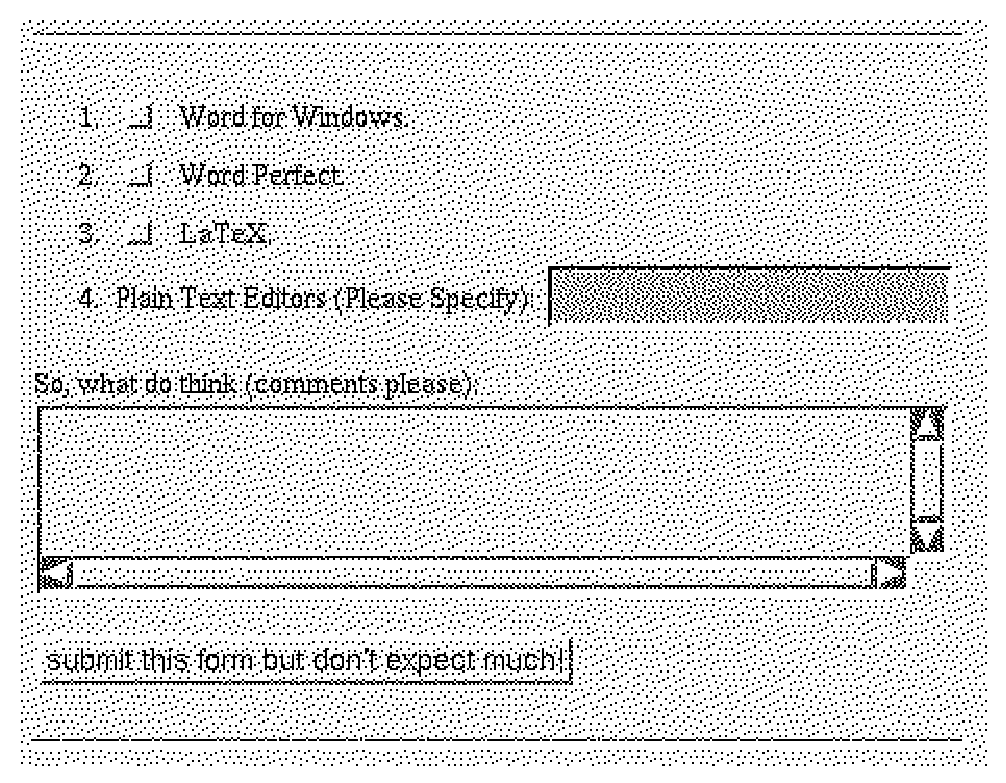
\psfig{file=eform.ps,width=4in}} \\
     Figure: An electronic form. Of course in the online version of this
document the form above would be active.
    \end{center}
\end{figure}
\end{latexonly}

{\bf Warning:} Avoid using LaTeX commands involving counters (e.g.
numbered figures or equations) in conditional text because this may 
disrupt the values of the counters in the electronic version.

% The argument here used to have a \label in its argument which caused
% the ``Contents'' page entry not to be hyperized.
\subsection{Conditional Text}
\label{sec:latexonly}
\index{latexonly} \index{htmlonly}
Conditional text can be specified using the environments {\tt latexonly} and {\tt
htmlonly}. These allow writing parts of a document which are intended
only for electronic delivery or only for paper-based delivery. 

This would be useful for example in adding a long description of a
multimedia resource in the paper version of a document. Such a
description would be redundant in the electronic version, as the user
can have direct access to this resource. 

Here is an example of the use of the {\tt latexonly} environment:

\begin{verbatim}
\begin{latexonly}
\begin{figure}
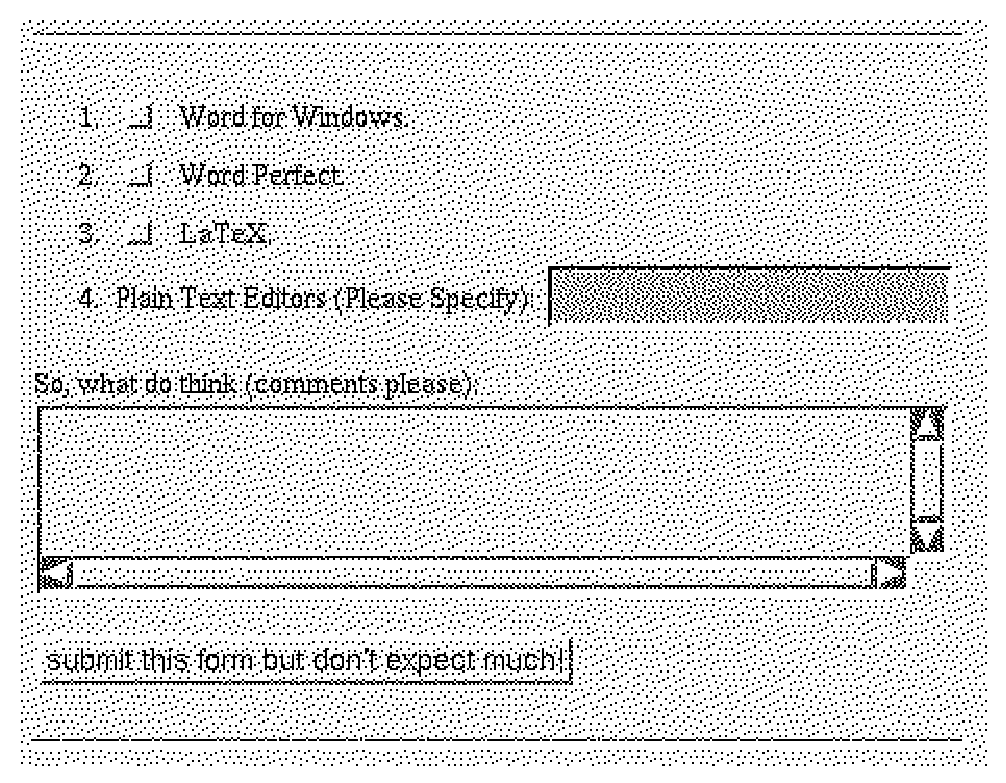
\psfig{file=eform.ps,width=4in}
\caption{An electronic form. Of course in the online version 
of this document the form above would be active!}
\end{figure}
\end{latexonly}
\end{verbatim} 

\subsection{Cross References Shown as ``Hyperized'' Text}

\index{cross-references}
In printed documents cross-references are shown through a {\em numerical
or symbolic indirection} e.g. ``see Figure 1'' (numeric indirection), or
``see section ``Changes'' (symbolic indirection).  \latextohtml can
mirror this mechanism using the same numeric or symbolic references,
or when these are
not appropriate by using iconic references.

In a hypertext document however, cross-references can be shown 
without any indirection just by highlighting a relevant piece of
text. This can make a document more readable as it removes unnecessary
information. 

A single new LaTeX command {\tt hyperref} can be used for
specifying how a cross-reference should appear both in the printed
document and in the hypertext version.

Assuming that the label \verb|sec:cond| is defined somewhere
in a document the command {\tt hyperref} which takes 4 arguments
can be used in the same document as follows:

\index{hyperref} \index{conditional text}
\begin{verbatim}
{\em Is the concept of
\hyperref
% This will be highlighted in the hypertext version
{conditional text}			% argument #1
% This will be shown in the printed version 
% followed by a numeric reference ...      
{conditional text (see Section }  	% argument #2
% ... followed by this text
{ for more information)} 		% argument #3
% This the common label 
{sec:cond}				% argument #4
a good idea? }
\end{verbatim}

Here is how it will be shown: \\
{Is the concept of
\hyperref
% This will be highlighted in the hypertext version
{conditional text}
% This will be shown in the printed version  
% followed by a numeric reference ...      
{conditional text (see Section }  
% ... followed by this text
{ for more information)} 
% This the common label 
{sec:cond}
a good idea? }

\begin{htmlonly}
In the printed version what would appear is: \\
{ Is the concept of conditional text (see Section XXX for more information) a good idea? }
\end{htmlonly}

\begin{latexonly}
In the hypertext version what would appear is:\\
{ Is the concept of \underline{conditional text} a good idea?} \\
Of course \underline{conditional text} would be an active hypertext link.
\end{latexonly}


Another command also defined in {\fn html.sty} is {\tt htmlref} 
which has the same effect as {\tt hyperref} during the conversion to
HTML.
It takes two arguments, some text and a label. In the HTML version the
text will be ``hyperized'' pointing to the label. In the paper version
the text will be shown as it is and the label will be ignored eg

\begin{small}
\begin{verbatim}
With {\tt htmlref} \htmlref{it's easy to make links}{fig:example}.
\end{verbatim}
\end{small}

\begin{htmlonly}
In the HTML version it will be shown as: \\
With {\tt htmlref} \htmlref{it's easy to make links}{fig:example}.
\end{htmlonly}
\begin{latexonly}
In the HTML version it will be shown as: \\
With {\tt htmlref} \underline{it's easy to make links}.
\end{latexonly}


\subsection{Customizing the Navigation Panel}
\index{navigation panel} \label{sec:navpanel}
The navigation panel is the strip containing ``buttons'' and text
that appears at the top
and perhaps at the bottom of each generated page and provides
hypertext
links to other sections of a document. Some of the
options and variables that control whether and where it should appear 
\hyperref{have already been mentioned}{have already been mentioned in 
Section }{}{navoptions}. 


A simple mechanism for appending customized buttons to the navigation
panel is provided by the command {\tt htmladdtonavigation}. This takes
one
argument which \latextohtml appends to the navigation panel. For
example,
\begin{verbatim}
\htmladdtonavigation
   {\htmladdnormallink
      {\htmladdimg{http://server/mybutton.gif}}
      {http://server/link}}
\end{verbatim}
will add an active button {\tt mybutton.gif} pointing to the specified location.


Apart from these facilities it is
also 
possible to specify completely what appears in the navigation panel 
and in what order. As each section is processed, \latextohtml
assigns relevant information to a number of global variables.
These variables are used by the subroutine {\fn navigation$\_$panel}
where the navigation panel is constructed as a string consisting of
these variables and some formatting information. 

This subroutine
can be redefined in a system or a user configuration file ({\fn
LATEX2HTMLDIR/latex2html.config} and {\fn HOME/.latex2html-init} 
respectively). {\em Any combination of text, HTML tags, 
and the variables mentioned below is acceptable}. 

The control panel variables are:

{\bf Iconic links (buttons)}
\begin{itemize}
\item PREVIOUS - points to the previous section 
\item UP  - points up to the "parent" section
\item NEXT - points to the next section
\item NEXT$\_$GROUP - points to the next "group" section
\item PREVIOUS$\_$GROUP - points to the previous "group" section
\item CONTENTS - points to the contents page if there is one
\item INDEX - points to the index page if there is one
\end{itemize}

{\bf Textual links (section titles)}
\begin{itemize}
\item PREVIOUS$\_$TITLE - points to the previous section
\item UP$\_$TITLE  - points up to the "parent" section
\item NEXT$\_$TITLE - points to the next section
\item NEXT$\_$GROUP$\_$TITLE - points to the next "group" section
\item PREVIOUS$\_$GROUP$\_$TITLE - points to the previous "group" section
\end{itemize}

If the corresponding section exists each iconic button will contain an
active link to that section. If the corresponding section does
not exist, the button will be inactive. If the section corresponding
to a textual link does not exist then the link will be empty.

The number of words that appears in each textual link
is controlled by the variable {\fn WORDS$\_$IN$\_$NAVIGATION$\_$PANEL$\_$TITLES}
which may also be changed in the configuration files.

Below is an example of a navigation panel 
(the ``.'' is the Perl string concatenation operator and ``\#''
signifies
a comment).

\begin{small}
\begin{verbatim}
sub navigation_panel {

    #  Start with a horizontal rule (3-d dividing line)
    "<HR> ".			
    
    # Now add few buttons with a space between them
    "$NEXT $UP $PREVIOUS $CONTENTS $INDEX $CUSTOM_BUTTONS" .
	    
    "<BR>\n" .		# Line break
	
    # If ``next'' section exists, add its title to the navigation panel
    ($NEXT_TITLE ? "<B> Next:</B> $NEXT_TITLE\n" : undef) . 
    
\end{verbatim}
\begin{verbatim}
    # Similarly with the ``up'' title ...
    ($UP_TITLE ? "<B>Up:</B> $UP_TITLE\n" : undef) . 
 
    # ... and the ``previous'' title
    ($PREVIOUS_TITLE ? "<B> Previous:</B> $PREVIOUS_TITLE\n" : undef) .
   
    #  Horizontal rule (3-d dividing line) and new paragraph  
    "<HR> <P>\n"		
}
\end{verbatim}
\end{small}

\subsection{Indicating Differences Between Document Versions} 

\latextohtml supports the {\fn changebar.sty} package by David B. Johnson 
(dbj@titan.rice.edu), for 
inserting ``change bars'' in a document in order to indicate 
differences from previous versions. This is a very primitive form of 
version control and there is much scope for improvement.


\subsection{Hypertext Links in Bibliographic References (Citations)}
If a report or a book that is cited (using the {\tt cite}) 
command is available (or there is information about it) on WorldWide
Web then it is possible to add the appropriate hypertext links
in your bibliographic database (the {\fn .bib}) file. 

Here is an example of a bibliographic entry for the original
LaTeX\cite{lamp:latex} book:

\begin{small}
\begin{verbatim}
@book{lamp:latex,
title = "LATEX User's Guide \& Reference Manual",
year = 1986 ,
author = "Leslie Lamport",
Publisher = "Addison-Wesley Publishing Company, Inc.",
note = "Online information on TeX and LaTeX is available at
\htmladdnormallink{http://curia.ucc.ie/info/TeX/menu.html}
{http://curia.ucc.ie/info/TeX/menu.html} and
\htmladdnormallink{http://es-sun2.fernuni-hagen.de/info2html?(latex.info)Top}
{http://es-sun2.fernuni-hagen.de/info2html?(latex.info)Top}"}
\end{verbatim}
\end{small}
No other
modifications are required for this to work - LaTeX and BibTeX 
should work as normal.

For those who use the Harvard style for references
\htmladdnormallinkfoot{there exists a special conversion
add-on package}{http://www.arch.su.edu.au/\~{}peterw/latex/harvard/}.

\subsection{Internationalization}
A special variable {\tt LANGUAGE\_TITLES} 
in the initialization or configuration files determines the language 
in which some section titles will appear. For example setting it to 
\begin{verbatim}
$LANGUAGE_TITLES = ``french'';
\end{verbatim}
will cause LaTeX2HTML to produce ``Table des mati\`{e}res'' instead of
``Table of Contents''.

The only languages currently supported are ``french'' and ``english''
but it is trivial to add support for another language in the
file {\fn latex2html.config}. As a guide here is the entry for 
the French titles:
\begin{verbatim}
sub french_titles {
 $toc_title = "Table des mati\\`eres";	
 $lof_title = "Liste des figures";
 $lot_title = "Liste des tableaux";
 $idx_title = "Index";
 $bib_title = "R\\'ef\\'erences";		
 $info_title = "\\`A propos de ce document..."; 
}
\end{verbatim}

In order to provide full support for another language you may also
want to replace the navigation buttons which come with \latextohtml 
(which are by default in
English)
with your own. As long as the new buttons have the same filenames as the
old ones there should not be a problem.

\subsection{Image Conversion}
\label{imgcon}

\latextohtml converts equations, special accents, external postscript
files, and LaTeX environments it cannot directly translate into 
inlined images. This section describes how it is possible to control
the final appearance of such images. For the purposes of the discussion below,

\begin{description}
\item[{\bf ``small images''}] will refer to equations, special accents and
any other image generating LaTeX commands, while 
\item[{\bf ``figures''}] will
apply  to any image generating LaTeX environments (eg figure, table,
minipage etc).
\end{description}

The size of all ``small images'' depends on a configuration variable
{\tt MATH\_SCALE\_FACTOR} which specifies how much to enlarge or 
reduce them in relation to their original size in the postscript 
version of the document. For example a scale factor of 0.5 will make all 
images half as big while a scale factor of 2 will make them twice as
big.
Larger scale factors result in longer processing times and larger 
intermediate image files. A scale factor will only be effective 
if it is greater than 0. 

The configuration variable {\tt FIGURE\_SCALE\_FACTOR} performs
a similar function for ``figures''. Both of these configuration 
variables are initially set to 1.6.

For finer control, several
parameters affecting the conversion of a single ``figure'' 
can be controlled
with the command {\tt htmlimage} which is defined in {\fn
html.sty}.
The one argument of {\tt htmlimage}
is a string of options separated by commas. The options are
\begin{verbatim}
scale = <scale factor>
external
thumbnail = <scale factor>
map = <image map URL>
\end{verbatim}

The {\tt scale} option allows control over the size of the final
image.

The {\tt external} option will cause the image not to be inlined 
(images are inlined by default). External images will be accessible
via a hypertext link. 

The {\tt thumbnail} option will cause a small inlined image to be 
placed in the caption. The size of the thumbnail depends on the
scale factor. The use of the {\tt thumbnail} option implies
the {\tt external} option. In order to be effective the command
{\tt htmlimage} and its options {\bf must be placed inside the
environment on which it will operate}.

The {\tt map} option will turn the inlined image into an 
\htmladdnormallink{active
image map}{http://wintermute.ncsa.uiuc.edu:8080/map-tutorial/image-maps.html}.

{\bf Example:}
The effect of the LaTeX commands below can be seen in the
\htmlref{thumbnail sketch of Figure}{fig:example} \ref{fig:example}.
\begin{small}
\begin{verbatim}
{\begin{figure}[tbh]
    \htmlimage{thumbnail=0.5}
    \centerline{
    \psfig{file=figure.ps,width=5in}}
    \caption{A sample figure showing part of a page generated by
\latextohtml containing a customized navigation panel (from the
\protect\htmladdnormallinkfoot{CSEP project}
{http://csep1.phy.ornl.gov/csep.html}).}
    \label{fig:example}
\end{figure}}
\end{verbatim}
\end{small}

The {\tt htmlimage} command is also often useful to cancel-out the
effect of the configuration variable {\tt FIGURE\_SCALE\_FACTOR}.
For example to avoid resizing a color screen snap despite 
the value of {\tt FIGURE\_SCALE\_FACTOR} it is possible to 
use {\tt htmlimage\{scale=0\}}.

\subsection{Figures, Tables and Arbitrary Environments}
\index{figures} These are here to show how the translator
handles figures, tables
and other environments. Compare the paper with the online version.

\index{tables}
\begin{table}[h]
\begin{center}
\begin{tabular}{||l|lr||}   \hline
gnats	&	gram	&	\$13.65  \\ \cline{2-3}
	&	each	&        .01	\\ \hline
gnu	& 	stuffed	&        92.50  
                \\  \cline{1-1} \cline{3-3}
emur	&		&	33.33   \\ \hline
armadillo	& frozen	&	8.99 \\ \hline
\end{tabular}
\end{center}
\caption{A sample table taken from \protect\cite{lamp:latex}}
\label{tab}
\end{table}

\index{numbered equations}
Here are some some automatically numbered right-justified equations
\begin{equation} 
\Phi_{l+1,m,n} = (\Phi+h\frac{\partial\Phi}{\partial x} +
\frac{1}{2}h^2\frac{\partial^2\Phi}{\partial x^2} +
\frac{1}{6}h^3\frac{\partial^3\Phi}{\partial x^3} + \ldots)_{l,m,n}
\end{equation}
with some gratuitously \'{a}cc\"{e}nted text in between them.
\begin{eqnarray}  \label{eq:demo}
\frac{\Phi_{l+1,m,n}-2\Phi_{l,m,n}+\Phi_{l-1,m,n}}{h^{2}} +
\frac{\Phi_{l,m+1,n}-2\Phi_{l,m,n}+\Phi_{l,m-1,n}}{h^{2}} + \nonumber \\
\frac{\Phi_{l,m,n+1}-2\Phi_{l,m,n}+\Phi_{l,m,n-1}}{h^{2}} = -I_{l,m,n}(v)
\end{eqnarray}

{\begin{figure}[tbh]
    \htmlimage{thumbnail=0.5}
    \centerline{
    \psfig{file=figure.ps,width=5in}}
    \caption{A sample figure showing part of a page generated by
\latextohtml containing a customized navigation panel (from the
\protect\htmladdnormallinkfoot{CSEP project}
{http://csep1.phy.ornl.gov/csep.html}).}
    \label{fig:example}
\end{figure}}

\section{Getting LaTeX2HTML}
\index{source code}
\begin{flushleft}
The \htmladdnormallink{source code can be obtained 
at http://cbl.leeds.ac.uk/nikos/tex2html/latex2html.tar.}
{http://cbl.leeds.ac.uk/nikos/tex2html/latex2html.tar}
or \htmladdnormallink{as a compressed archive at http://cbl.leeds.ac.uk/nikos/tex2html/latex2html.tar-gz}{http://cbl.leeds.ac.uk/nikos/tex2html/latex2html.tar-gz}
The source code is also available 
via anonymous FTP at 
\htmladdnormallink{ftp://ftp.tex.ac.uk/pub/archive/support/latex2html}{ftp://ftp.tex.ac.uk/pub/archive/support/latex2html}
or
\htmladdnormallink{ftp://sunsite.unc.edu/pub/packages/infosystems/WWW/tools/translators/latex2html}{ftp://sunsite.unc.edu/pub/packages/infosystems/WWW/tools/translators/latex2html}.
Other FTP sites nearer to you can be found using {\fn Archie}
at
\htmladdnormallink{http://hoohoo.ncsa.uiuc.edu/archie.html}{http://hoohoo.ncsa.uiuc.edu/archie.html}
or 
\htmladdnormallink{http://www.pvv.unit.no/archie/}{http://www.pvv.unit.no/archie/}
(faster).

{\bf Warning:} Some FTP sites may not carry the latest version.

Updates and patches are posted on the \latextohtml server at
\htmladdnormallink{http://cbl.leeds.ac.uk/nikos/tex2html/doc/latex2html/latex2html.html}{http://cbl.leeds.ac.uk/nikos/tex2html/doc/latex2html/latex2html.html}

\end{flushleft}

If you get the {\tt tar} version, save it into a file, say {\tt latex2html.tar}
and then extract the files with 
\begin{verbatim}
% tar xvf latex2html.tar
\end{verbatim} 

You should then have the following:
\begin{itemize}
\item A {\fn README} file.
\item A {\fn Changes} file.
\item The {\fn latex2html} Perl program.
\item A \index{texexpand} {\fn texexpand} Perl program \footnote{Written 
by Robert S. Thau $<$rst@edu.mit.ai$>$.}.
\item A {\fn latex2html.config} configuration file.
\item An {\fn install-test} installation and testing Perl script.
\item A {\fn dot.latex2html-init} sample initialization file.
\item A {\fn html.sty} style file.
\item A {\fn pstogif} perl script.
\item Two {\fn pstoppm.ps} files.
\item A {\fn docs/} subdirectory containing a version of this
manual.
\item An {\fn icons/} subdirectory containing various icons.
\item A {\fn styles/} subdirectory containing Perl code for handling
some style files.
\end{itemize}
\section{Requirements}
\index{requirements}
The translator makes use of several utilities all of which 
are freely available on most platforms. \htmladdnormallinkfoot{You may use 
{\fn Archie} to find the source code of any utilities you might need.}
{http://www.pvv.unit.no/archie/}

The requirements for using \latextohtml 
depend on the kind of translation you would like to perform, as follows:

\begin{enumerate}
\item {\bf LaTeX commands but without equations, figures, tables, etc.} \hfill
\begin{itemize}
\item \htmladdnormallink{{\fn Perl}}{ftp://ftp.uu.net/languages/perl/} 
(version 4.0 - RCSfile: perl.c,v - Revision: 4.0.1.8 - Date:
1993/02/05 19:39:30 - Patch level: 36)

{\bf Warning:} You really DO need Perl at patch level 36 or later.
Versions of \latextohtml earlier than 0.7a4 work {\bf only} with 
Perl 4 at patch level 36. Later versions of \latextohtml work 
both with Perl 4 at patch level 36 and Perl 5. {\bf No} version 
of \latextohtml will work  with Perl 4 at earlier patch levels.

\item {\fn DBM} or {\fn NDBM}, the Unix DataBase Management system.
\end{itemize}

\item {\bf LaTeX commands with equations, figures, tables, etc.} \\
As above plus
\begin{itemize}
\item {\fn latex},
\item  \htmladdnormallink{{\fn dvips}}
{ftp://ftp.tex.ac.uk/pub/archive/dviware/dvips}
(version  5.516 or later) or {\fn dvipsk}.
\item {\fn gs} (Ghostscript version 2.6.1 or later). 
\item The \htmladdnormallink{{\fn
pbmplus}}{ftp://ftp.x.org/R5contrib/}
OR \htmladdnormallink{{\fn
netpbm}}{ftp://ftp.x.org/R5contrib/}
library.
Some of the filters in those libraries are used during the postscript to
GIF conversion. 
\end{itemize}

\item 
{\bf \htmladdnormallinkfoot{Transparent inlined images}{http://melmac.corp.harris.com/transparent\_images.html}}\\
If you dislike the ugly white background color of the
generated inlined images then you should get either 
the {\fn netpbm} library (instead of the older {\fn pbmplus}) OR
install the
\htmladdnormallinkfoot{{\fn
giftrans}}{ftp://ftp.rz.uni-karlsruhe.de/pub/net/www/tools/giftrans.c}
filter by Andreas Ley $<$ley@rz.uni-karlsruhe.de$>$. 
Version 1.10.2 is
known to work without problems but later versions should also be OK.

\end{enumerate} 

If {\fn ghostscript} or the {\fn pbmplus} (or {\fn netpbm}) library are not
available it
is still possible to
use the translator with the {\tt -no\_images} option. 

If you intend to use any of the special features of the translator (see Page \pageref{special})
then you have to include the 
{\fn html.sty} file in any LaTeX documents that use them. 

Because by default the translator makes use of inlined images in the final 
HTML output, it would be better to have a viewer which supports 
the {\tt $<$IMG$>$} tag, such as \htmladdnormallink{NCSA 
Mosaic}{http://www.ncsa.uiuc.edu/SDG/Software/Mosaic/Docs/help-about.html}.
If only a character based browser is available or if you want the
generated
documents to be more portable then the translator can be used
with the 
\hyperref{{\tt -ascii$\_$mode} option}{{\tt -ascii$\_$mode} option (See
Section }{ )}{asciimode}. 

\section{Installing LaTeX2HTML}

To install \latextohtml you {\bf MUST} do the following:

\begin{enumerate}
\item {\bf Specify where Perl is on your system}. \\
In each of the files {\fn latex2html}, {\fn texexpand} {\fn pstogif}
and  {\fn install-test},
modify the first line saying where Perl is on your system. 

Some system administrators do not allow Perl programs to run as shell
scripts. This means that you may not be able to run any of the above
programs. {\em In this case change the first line in each of these
programs from}
\begin{verbatim}
#!/usr/local/bin/perl
\end{verbatim}

{\em to}

\begin{verbatim}
: # *-*-perl-*-*
    eval 'exec perl -S  $0 "$@"'
    if $running_under_some_shell; 
\end{verbatim}

\item {\bf Specify where the external utilities are on your system.} \\
In the file {\fn latex2html.config} give the correct pathnames for 
some directories (the {\fn latex2html} directory and the {\fn 
pbmplus} or {\fn netpbm} library) and some executables ({\fn latex, dvips, gs}). 
Note that it is
possible 
to use \latextohtml even
if you don't have some of the external utilities.

While you're at it you may want to change some of the default 
options in the same file.

\item {\bf Run {\fn install-test}.} \\
This Perl script will make some changes in the {\fn latex2html} file
and then check whether the pathnames to any external utilities
(specified during the previous step) are correct. It will not actually
install the external utilities. 

Don't forget to make {\fn
install-test} executable (using the {\fn chmod} command) before
using it if necessary. You may also need to make the files
{\fn pstogif}, {\fn texexpand} and {\fn latex2html} executable 
if {\fn install-test} fails to do it for you.

If for any reason you have trouble running {\fn install-test}
do not despair. Most of what it does is to do with checking
your installation rather than actually installing anything.
To do a {\bf manual installation} just change the variable
{\tt LATEX2HTMLDIR} in the beginning of the file {\fn latex2html}
to point to the directory where the \latextohtml files can be found.
\end{enumerate}

This is enough for the main installation but you may also 
want to do some of the following:
\begin{itemize}

\item {\bf To use the new LaTeX commands which are defined in {\fn html.sty}:} \\
Make sure that LaTeX knows where the html.sty
file is, either by putting it in the same place as the other style files on
your system, or by changing your TEXINPUTS shell environment variable,
or by copying html.sty in the same directory as your LaTeX source file.

\item {\bf To set up different initialisation files:} \\
For a ``per user'' initialisation file, 
copy the file {\fn dot.latex2html-init} in the home directory
of any user that wants it, modify it according to her preferences and
rename it as {\fn .latex2html-init}. At runtime, both the {\fn 
latex2html.config} file and {\fn \$HOME/.latex2html-init} file will be
loaded, but the latter will take precedence.

You can also set up a ``per directory'' initialisation file by 
copying a version of {\fn .latex2html-init} in each directory you
would like it to be effective. An initialisation file
{\fn /X/Y/Z/.latex2html-init} will take precedence over all other
initialisation files if {\fn /X/Y/Z} is the ``current directory'' when
\latextohtml is invoked.

\item {\bf To make your own local copies of the \latextohtml icons:} \\
Please copy the {\fn icons} subdirectory to a 
place under your WWW tree
where they can be served by your server.
Then modify the value of the {\fn \$ICONSERVER} variable in 
{\fn latex2html.config} accordingly. 

{\bf Warning:} If you cannot do that
bear in mind that these icons will have
to travel from Leeds!!! Also, your documents will depend on our
server being operational in the first place.

\item  {\bf To make your own local copy of the \latextohtml
documentation:} \\
This will also be a good test of your installation. 
To do it run \latextohtml on the file {\fn docs/manual.tex}.
You will get better results if you run LaTeX first on the 
same file in order to create some auxiliary files.

\item {\bf To join the community of \latextohtml users:} \\
More information on a mailing list, discussion archives, bug reporting
forms and more is available at \\
\htmladdnormallink{http://cbl.leeds.ac.uk/nikos/tex2html/doc/latex2html/latex2html.html}
{http://cbl.leeds.ac.uk/nikos/tex2html/doc/latex2html/latex2html.html}
\end{itemize}

\section{Changes from Previous Versions}
The \htmladdnormallink{previous versions of the
translator and some patches}{http://cbl.leeds.ac.uk/nikos/tex2html/previous-versions}
are available. A \htmladdnormallink{detailed list of changes}
{http://cbl.leeds.ac.uk/nikos/tex2html/doc/Changes.txt}
which includes full credits to all who have contributed 
bug fixes or other code is also available with the
\latextohtml distribution in the file {\fn Changes}.


\subsection{Changes upto v95}
\begin{description}
\item[{\bf Much improved inlined equation baseline alignment!}]
(Thanks to Mark Segal $<$segal@spud.asd.sgi.com$>$)
Inlined equation bitmaps are now aligned correctly depending 
on whether they contain subscripts, superscripts etc. 
\item[{\bf Support for internationalization}]
(Thanks to Martin Boyer $<$gamin@ireq-robot.hydro.qc.ca$>$)
A global variable {\tt LANGUAGE\_TITLES} can now be used to change the
language in which some section titles (eg ``Table of Contents'') are
printed. It is also very easy to add support for more languages.
\item[{\bf Compatibility with Perl 5}]
\item[{\bf More efficient implementation}]
There has been a major overhaul of the way the source text is parsed
and analysed in order to reduce the memory requirements of this
process.

This has been achieved by spawning off separate Unix processes to deal
with each of the {\tt input}'ed or {\tt include}'d files. As each
process
terminates all the space that it used is reclaimed. 
Asynchronous communication between processes takes place using 
the Unix DataBase Management system (DBM or NDBM) 
which should be present
on your system.

{\bf To take advantage of these changes}, 
it is necessary to split the source text 
into more than one files which can be assembled using the \LaTeX
{\tt input} or {\tt include} commands.


\item[{\bf ``Off-line'' Image Generation}]

Two new options {\tt -no\_images} and {\tt  -images\_only} allow
``off-line'' image conversion. The advantage of using these options is 
that the translation can be allowed to finish even when there are
problems with image conversion. In addition it may be possible to 
fix manually any image conversion problems and then run \latextohtml 
again just to integrate the new images without having to translate
the rest of the text. More instructions on how to do this are
included in the ``Troubleshooting'' section of the \latextohtml
manual.

Can now use either the {\fn pbmplus} or the {\fn netpbm} libary.
If {\fn netpbm} is used then it is no longer necessary to get and
install {\fn giftrans} in order to generate transparent inlined 
images.

Also, a new option {\tt map=$<$image map URL$>$} in the 
command {\tt htmlimage} can turn an included postscript image into an active
image map.

\item[{\bf New options}] \hfill
\begin{description}
\item [-no\_images]
Do not attempt to produce any inlined images. 
The missing images can be generated "off-line" by restarting \latextohtml
with the option {\tt -images\_only}.
\item [-images\_only]
Try and convert any inlined images that were left over from previous
runs of \latextohtml. 
\item [-no\_reuse]
Do {\bf not} reuse images generated during previous translations.
(This will enable the initial interactive session during which the user is
asked whether to reuse the old directory, delete its contents or quit)
\item [-no\_subdir]
Place the generated HTML files  in the 
current directory. The default behaviour is to create (or reuse)
another file directory.
\item [-ps\_images]
Use links to external postscript images rather than inlined GIF images.
\end{description}
\item[{\bf Several small changes and bug fixes}] \hfill
\begin{itemize}
\item It is no longer necessary to get {\fn Giftrans} if {\fn NETPBM}
is available
\item Fixed problems with support for {\fn german.sty}
\item Fixed problems with multiple bibliographies. Each bibliography
is now treated as a separate section.
\item Added support for ``dotless i's and j's''.
\item  Fixed to resolve figure and table numbers when captions contain
accented characters.
\item Added support for hierarchical indices with duplicate index keys
\item Fixed problem with HTML encodings of ISO-LATIN1 characters   
creeping into converted images of figures and tables.
\item  Added new global variable {\tt PAPERSIZE}
to make it easier to change the default behavior when converting large images
\item A new configuration variable ({\tt TRANSPARENT\_IMAGES}) can be 
used to stop any inlined images generated from "figure" environments
from being transparent.
\item Fixed problem which occurs when {\fn getcwd.pl} is not part of the
Perl library.
\item The option {\tt -address ""} is now valid.
\item Fixed a problem with tables of contents.
\item Fixed problem with the use of the {\tt finger} command when
trying to find out the name of the user.
\item Added some support for {\tt tabbing} environments.
\item HTML heading elements no longer contain other markup.
\item Fixed problem with optional argument in citation commands
\item Added some more support for LaTeX2e.
\item Fixed problem with displayed equations forcing all the remaining
equations to be displayed.
\item Fixed bug with converting postscript images containing more than
256 colors.
\end{itemize}
\end{description}

\subsection{Changes upto v0.6.2}

\begin{description}
\item[{\bf Image Conversion}] \hfill
\begin{itemize}
\item The {\fn pstogif} script has been rewritten in Perl and it
now accepts more options for specifying color depth, scale factors
and pixel density.
\item LaTeX {\tt figure} and other environments are now processed
in 24-bit color.
\item Figure and table captions are now converted into HTML
rather than becoming part of the inlined image. This means that 
any cross-references in the captions will become active.
\item It is now possible to control for each generated image:
\begin{itemize}
\item its size 
\item whether it should be inlined or left as an external image
\item if left as an external image whether it should be accessible
via a \htmlref{{\bf generated thumbnail sketch}}{fig:example}
or a textual hypertext link
\end{itemize}
These options are available from a new LaTeX command defined in {\fn
html.sty} called {\fn htmlimage}. 

\item Equations and other inlined images are converted into
transparent GIFs rather than XBMs. {\bf This makes it possible 
to reduced their storage requirements to about 1/6th of what was
previously required!}
\item The default size of equations and other small inlined 
images can be changed
by setting the variable {\tt MATH\_SCALE\_FACTOR} in the
configuration files.
\item The default size of figures, tables, and other large
inlined images can be changed by setting the variable 
{\tt FIGURE\_SCALE\_FACTOR} in the
configuration files.

\item Dvips is now called with the {\tt -M} option which stops it
from invoking {\tt METAFONT}.
\end{itemize}

\item[{\bf Optimization}] \hfill
\begin{itemize}
\item Some effort has gone into reducing the amount of memory required
during conversion. {\bf The impact of these changes can be very
significant}.
In particular, files
containing large numbers of LaTeX commands (eg {\fn .aux} or {\tt .bib}) 
files are handled much better.
\end{itemize}

\item[{\bf Backwards Incompatible Changes}] \hfill
\begin{itemize}
\item The option {\tt -allbitmaps} has been removed. This is no
longer necessary as \latextohtml can now generate transparent
GIF images.
\item The definition of the command {\tt htmladdnormallink} in the 
file {\fn html.sty} has changed and the URL will no longer appear
as a footnote in the paper (DVI) version. The translation of
this command into HTML is {\bf not} affected. 

The previous functionality can be obtained with a new command
{\tt htmladdnormallinkfoot} which will add the URL as a footnote
in the paper version.
\item The script {\fn pstoxbm} is no longer distributed as it is not
used.

\end{itemize}

\item[{\bf Bug Fixes}] \hfill
\begin{itemize}
\item The {\fn install-test} script now recognizes version
numbers correctly and gives better warnings. It also makes
executable any scripts that need to be so. 
\item Stopped using the {\tt nslookup} program to try and guess
e-mail addresses (they were used in signing each generated page). 
This has been replaced with a simple call 
to {\tt finger}.
\item Fixed problem which could cause ``Parameter overflow'' in 
TeX during image conversion.
\item The {\fn texexpand} script has been changed extensively.
Some nasty looping problems are now avoided, and the tracking
down of included files has been improved.
\item Some reported incompatibilities with some Unix shells
(bash,OSF) have been fixed.
\item Displayed equations now appear correctly on separate
lines and are right justified.
\item Fixed bug with nested environments.
\item Fixed problem which caused the wrong numbers to be assigned
to sections with the same titles when the {\tt -show\_section\_titles}
is used (thanks to Brian  Toonen $<$toonen@mcs.anl.gov$>$).
\item Fixed problem with the {\tt hyperref} command which
caused the wrong ``hyperized'' text to appear in the final document.
\item {\tt item} optional arguments can now contain one level of
nesting eg {\tt item[[First Choice]]}.
\item Fixed problems with the ``image caching and reuse'' mechanism 
which avoids converting images unnecessarily..
\end{itemize}

\item[{\bf Other Changes}] \hfill
\begin{itemize}
\item LaTeX2HTML now generates $<$meta$>$ HTML tags which can be used
by \htmladdnormallinkfoot{indexing scripts}
{http://www.ai.mit.edu/tools/site-index.html}
 which generate information for the \htmladdnormallinkfoot{ALIWEB}
{http://web.nexor.co.uk/aliweb/bin/aliwebsimple.pl} 
search and retrieval tool. The information in the $<$meta$>$ tags
contains
the title of each separate HTML file. 
\item A new configuration variable {\tt DEBUG} can be used to preserve
intermediate files for debugging. 
\item Some problems with respect to compatibility with the HTML2.0 
standard have been addressed. No more ``unquoted attribute value literals''.
\item All the navigation icons are now ``lynx friendly''; their
{\tt ALT} attribute now has a meaningful value.
\item A new LaTeX command {\fn htmlref} makes it a lot simpler
to create hypertext links intended only for the HTML version of
the document.
\item {\fn DVIPSK} is now recognized by the installation script
\item Added support for the {\fn changebar.sty} file by 
David B. Johnson (dbj@titan.rice.edu).
\item It is no longer necessary to add style file names into the 
{\tt DONT\_INCLUDE} variable as \latextohtml now does not
attempt to translate file included files ending in {\tt .sty}.
\item The small invisible bitmaps that used to mark anchors have been
replaced with the invisible character \verb|&#160;|.
\item It is no longer necessary to use full pathnames when
including external postscript files.
\item If a file {\fn .latex2html-init} is found in the ``current
directory'' then this will be loaded automatically after loading the
other default configuration files.
\item Changed the naming convention of generated HTML files. The
``top'' document is {\fn $<$FILE$>$.html} as before but all other ``nodes''
are named {\fn nodeN.html} where {\fn N} is an integer. Also, the file
containing
the footnotes is now called {\fn footnode.html}.
\item A special extension to \latextohtml for those who use the 
Harvard style for references can be obtained from
\htmladdnormallink{http://www.arch.su.edu.au/\~{}peterw/latex/harvard/}{http://www.arch.su.edu.au/\~{}peterw/latex/harvard/}.
\end{itemize}
\end{description}


\subsection{Changes upto v0.5.3}
\begin{itemize}
\item The files {\fn LATEX2HTMLDIR/styles/german.perl} and 
{\fn LATEX2HTMLDIR/styles/makeidx.perl} have been fixed
so that they are consistent with changes in the main script.
\item A problem with disappearing spaces after some equations
and other environments has been fixed.
\end{itemize}
\subsection{Changes upto v0.5.1}
\begin{description}
\item[{\bf Navigation Panel}]
The \hyperref{navigation panel}{navigation panel (see section
}{)}{sec:navpanel}
is now fully configurable and much better looking.
\item[{\bf Automatic Signatures}]
The signatures at the bottom of each page are now constructed
using {\fn nslookup} (Thanks to Alberto Accomazzi
$<$alberto@cfa.harvard.edu$>$)
\item[{\bf Numerous fixes including...}] \hfill
\begin{itemize}
\item ``dead'' {\fn next$\_$page} buttons when the {\fn -split} option
was used, and
\item internal \latextohtml markers appearing in section titles.
\end{itemize}
\end{description}

\subsection{Changes upto v0.4}
\begin{description}
\item[{\bf Accents and Special Characters}]
LaTeX accent commands, special characters and accent commands defined
in {\fn german.sty} are translated to equivalent ISO-LATIN-1
characters when that is possible (partly thanks to code supplied
by Franz Vojik $<$vojik@de.tu-muenchen.informatik$>$).
\item[{\bf Auto-loading of Style-Specific Code}]
The translator now supports a 
\hyperref{mechanism for including Perl code extensions}{mechanism for
including Perl code extensions (see Section }{)}{sec:sty}
which are specific to particular style files. 


This mechanism will help to keep the core script smaller as well as make
it easier for others to contribute and share solutions on  
how to translate specific style files. The current distribution includes the files
{\fn german.perl}, {\fn french.perl}, {\fn html.perl} and {\fn makeidx.perl}.
\item[{\bf Installation and Testing}]
To make it easier to install the translator for more than one user
there is now a configuration file ({\fn
LATEX2HTMLDIR/latex2html.config}) which contains installation specific 
information and default values for the various options. 
This makes it unnecessary to have a {\fn HOME/.latex2html-init} for
each user.
If a user does have a  {\fn HOME/.latex2html-init} then this will be
loaded after {\fn
LATEX2HTMLDIR/latex2html.config}.

A new Perl script ({\fn install-test}) is now available with the distribution
which will install the translator, and then perform some tests on the
availability
of some external
programs giving, appropriate warnings.
\item[{\bf Navigation Panel Extensions}]
The following new links have been added to the navigation panel which
appears in each page
(where this is appropriate):
\begin{itemize}
\item a link to the next ``logical'' page (this allows reading each
page in the same order as with a paper-based version - as opposed to
structure navigation)
\item a link to the previous ``logical'' page 
\item a link to the table of contents
\item a link to the index 
\end{itemize}
\item[{\bf HTML Style File Extensions}]
The HTML style file {\fn html.sty} now includes definitions of new 
environments for:
\begin{description}
\item[Inclusion of Raw HTML]
A new LaTeX environment {\tt rawhtml} allows
arbitrary
HTML tags to be included in a LaTeX document. This is useful for
taking
advantage of HTML+ features as they become available (e.g. interactive
forms).
The HTML commands are ignored when producing the DVI version of the
document.
\label{sec:cond}
\item[Conditional Text]
The new environments {\tt latexonly} and {\tt htmlonly} allow their
contents to appear only in final DVI or in the HTML version of a
document respectively. 

A new command {\tt hyperref} can be used to specify the way in
which cross-references should be shown in the DVI version and the
HTML version of the document.
\end{description}
\item[{\bf Right Justification of Equations}]
The translator
adds enough whitespace at the beginning of each equation bitmap
to push it to the right-hand margin. The width of each line can be
set in the configuration file using the variable {\tt LINE$\_$WIDTH}.
\item[{\bf Inlined Images}]
All inlined images are now generated by calling {\tt latex} and {\fn
dvips} only once
at the end of the conversion process (but each generated image still
has to be filtered individually). Also, a warning is given if an 
image cannot be converted.
\item[{\bf Numeric Labels}]
The original (LaTeX generated) numeric labels are used instead of
the arrow navigation icon for cross-references where possible.
To do this the translator uses the information in the 
{\fn aux} file which is generated by \LaTeX. If the {\fn aux} file
is out of date a warning is given.
\item[{\bf New Options}] \hfill
\begin{description}
\item[{\tt -auto$\_$navigation}]
This puts a navigation panel 
at the top of each page as usual. But if the page exceeds a
user-settable  
number of words (the default is 450 words) 
then a navigation panel is also placed at the end of
the page. This option is active by default.
\item[{\tt -index$\_$in$\_$navigation}]
Adds a link to the index in the navigation panel.
\item[{\tt -contents$\_$in$\_$navigation}]
Adds a link to the table of contents in the navigation panel.
\item[{\tt -next$\_$page$\_$in$\_$navigation}]
Adds a link to the next ``logical'' page in the navigation panel.
\item[{\tt -previous$\_$page$\_$in$\_$navigation}]
Adds a link to the previous ``logical'' page in the navigation panel.
\item[{\tt -bottom$\_$navigation}]
This puts a navigation panel at the bottom of each page.
\item[{\tt -top$\_$navigation}]
This puts a navigation panel at the top of each page (the default).
\item[{\tt -show$\_$section$\_$numbers}]
This allows each section (page) title to be numbered in the same 
way that it would be numbered by \LaTeX. This requires 
an up to date {\fn aux} file (generated by running \LaTeX) and that 
each title is unique. If the {\fn aux} file is not up to date then a 
warning is given.
Unfortunately if 
the title contains inlined images the numbering for that title will
be lost. 
\item[{\tt -reuse}]
This allows images generated during previous invocations of
the translator to be ``reused'' without going through the initial 
interactive session. The same behavior is obtained by setting
the variable {\tt REUSE} to 1 (the default) in the configuration file.
Note that images which may depend on contextual information (e.g. numerical
labels) cannot be reused and are always re-generated. 
\end{description}
\item[{\bf Bug Fixes and Minor Changes}] \hfill
\begin{itemize}
\item The links from the table of contents in single page documents (created using
the option {\tt -split 0}) is now working as expected.
\item Newlines are translated to the $<$BR$>$ tag.
\item Fixed some problems in dealing with new command macros.
\item {\fn texexpand} now respects commented {\tt input} and {\tt
include} commands. Also (thanks to Franz Vojik
$<$vojik@de.tu-muenchen.informatik$>$), it 
now looks in subdirectories when expanding
files.
\item The ALIGN attribute of inlined images is now BOTTOM instead of
TOP.
\item Fixed problem with the environment variable {\tt TEXINPUTS}.
\item Added some support for optional user-defined labels (bullets) in
list environments.
\end{itemize}
\end{description}

More details on all the changes are available in the file 
{\fn LATEX2HTMLDIR/Changes}.

\subsection{Changes upto v0.3.1}
These changes are mostly due to patches contributed by Robert S. Thau
$<$rst@ai.mit.edu$>$:
\begin{itemize}
\item Nested environments with the same name are now dealt with
properly.
\item Commands that are passed to LaTeX for processing which have 
environments in their arguments (e.g. a {\tt parbox} command which 
an {\tt itemize} environment as an argument) are now
processed correctly. A general mechanism for users to 
specify the syntax of commands that should be passed to LaTeX 
is described in Page \pageref{pass}.
\item Fixed a problem with recognizing the {\tt special} command.
\item Fixed bug in the generation of the index.
\end{itemize}

\subsection{Changes upto v0.3}
\begin{description}
\item [{\bf Image Recycling}]
Images for equations, tables, figures, special characters etc. generated by
the translator are recognised  during subsequent runs.
The user is then asked whether old images should be reused
(or whether the old images should be deleted and regenerated).
This offers tremendous improvements in speed after an initial
successful translation.

\item [{\bf Cross-References Between (Local or Remote) Documents}]
Cross-references between 
two or more documents (possibly on remote locations) can be
established via symbolic labels
which are independent of the physical realisation of these documents. 

Such cross-references will be maintained with a simple
re-translation\footnote{This is true for documents under the same
server but for remote documents a little more is required (see 
the \hyperref{example}{example in Section}{}{crossrefs})}
even after one or more of the documents have been broken into
different physical parts or moved.

The mechanism is based on the 
\hyperref{new commands}{new commands (see Section }{ )}{external}
{\tt externallabels} and {\tt externalref} which are an extension of the simple 
{\tt label-ref} pairs. 

\item [{\bf New Options}] \hfill
\begin{description}
\item [{\tt external$\_$images}] This provides hypertext links to where
generated images (for equations, tables, figures etc) are stored
externally. (The default is to ``inline'' generated images in the main body 
of the text.)
\item [{\tt ascii$\_$mode}] This switches all the navigation icons to their
ascii equivalents. Also generated images are stored externally as with the 
{\tt external$\_$images} option above. The {\tt ascii$\_$mode} option
makes documents more portable as it allows them to be
viewed on browsers that do not support inlined images.
\end{description}
\item [{\bf Special Command Style File}] A style file \htmladdnormallink{{\fn html.sty}} 
{http://cbl.leeds.ac.uk/nikos/tex2html/doc/html.sty.txt} is now included in the
distribution. This contains the definitions (syntax) of some 
special LaTeX commands mainly for providing external hypertext
links.
This should be included in LaTeX files that use the any 
\hyperref{hypermedia extensions}{hypermedia extensions (see Section}{ )}{special}.

\item [{\bf Minor Changes and Bug Fixes}] \hfill
\begin{itemize}
\item Equations, equation arrays and theorems are now numbered
correctly even when they are individually passed to LaTeX for
processing.
\item Fixed problem with {\tt label} commands appearing in section
headings.
\item Fixed problems with verbatim environments, bibliography items,
generated file names, the options {\tt nolatex} and {\tt
no$\_$navigation}, the {\tt thanks command}, the name of an HTML tag
($<$HEAD$>$), 
\item The appearance of footnotes has been improved.
\item Some inconsistencies in the {\fn pstoxbm} and {\fn pstogif}
 scripts have been fixed.  
\item Parts of the documentation have been rewritten, restructured and
some new sections have been added. 
\end{itemize}
\end{description}

{\bf The following were contributed by Robert S. Thau
$<$rst@ai.mit.edu$>$:}

\begin{description}
\item [{\bf New Texexpand}]
This fixes problems with the standard version and 
handles the inclusion of style files which need to processed by the 
translator. Appropriate modifications to the main script were also 
made to work with new version of {\fn texexpand}. 

\item [{\bf Handling of Raw \TeX}]
Added support for simple raw TeX commands such as  
{\tt special} and simple instances of {\tt def}\footnote{Where
``simple'' is defined roughly 
as ``they could have used {\tt newcommand}, but didn't''.}. 
For the messier cases, 
the definition is scooped up and moved to the preamble.  This allows 
the translator to handle the simple, but nonstandard, postscript figure inclusion
macros as well as an awful lot of other stuff done with gratuitous 
{\tt defs}.
\item [{\bf More Options}] \hfill
\begin{description}
\item [{\tt dont$\_$include}]
This can be used  to specify style files that
should not be included in the translation.
\end{description}
\item [{\bf Other Changes}] \hfill
\begin{itemize} 
\item Added support for nested math mode expressions and general
list environments in order to handle {\em the document from Hell!!!}.
\item Fixed problems in the translation of 
bibitems, the substitution of macro definitions, and the processing of
unrecognized commands in the preamble.
\end{itemize}
\end{description}
\subsection{Changes upto v0.2}
\begin{itemize}
\item Added a command line option
to switch off the navigation links
at the top of each page.
\item The navigation icons are now part of the distribution.
\item Added a customizable separator between the main body of the text
in a page and the child links from that page.
\item The order of the navigation keywords at the top of each page is
the same as that of the navigation icons.
\item The arguments of {\tt verbatim} environments are now translated
into fixed width fonts.
\item A warning is given if a {\tt bbl} (bibliography) file is 
needed but not found.
\item The installation is now (mostly) done by setting variables in 
just one file.
\item The {\fn pstoxbm} script now uses environment variables
set in the initialization file.
\item Fixed bug in translating sequences of special HTML characters
(e.g. \&, $<$, etc.)
\item Fixed bug in the handling of the \verb|$$|-form of the dislay
math environment.
\item Fixed bug in the handling of the *-forms of environments.
\item Added sections on how to embed hyperlinks in a LaTeX document 
(see Page \pageref{sec:hyper}) and on how to extend the translator
(see Page \pageref{sec:extend}) in the documentation.
\end{itemize}

\subsection{Changes upto v0.1.1}
\begin{itemize}
\item Fixed bug about empty lines being inserted in environments that
cannot tolerate them (e.g. {\tt math}).
\item Changed the format of inlined images coming back from LaTeX
from GIF to XBM. This looks better on grayscale and color monitors.
\item Fixed problem with commands being passed on to LaTeX  after
their
arguments had been translated (this affects the commands 
{\tt psfig}, {\tt fbox}, {\tt framebox}, and {\tt parbox}).
\end{itemize}
\section{Known Problems}
\index{problems} \index{bugs}
Here are some of the problems of the current version:
\begin{description}
\item [{\bf Correctness and Efficiency} \index{efficiency}]
The translator cannot be guaranteed to perform as expected.
Several aspects of the implementation need
optimization and improvement. Apart from possible bugs the translator 
may place heavy demands on your resources.
\item [{\bf Unrecognized Commands and Environments} \index{unrecognized commands}]
Unrecognized commands are ignored and any arguments are left in the
text. Unrecognized environments are passed to LaTeX  and the result is
included in the document as one or more inlined images.
\item [{\bf Cross-references}\index{cross-references}]
References in environments that are passed to LaTeX  for processing
(e.g. a {\tt cite}, or a {\tt ref} command), are not processed
correctly.
{\tt label} commands are handled correctly.
\item[{\bf Order Sensitive Commands}]
Commands which affect global parameters during the translation,
and are sensitive to the order in which they are processed may
not be handled correctly. In particular, counter manipulation
(e.g. {\tt newcounter, setcounter, stepcounter}, etc) 
commands may cause problems.
\item [{\bf Index}\index{index}]
The translator generates its own index by saving the arguments  of 
the {\tt index} command. The contents of the {\tt theindex}
environment are ignored.
\item[{\bf New Definitions}\index{new definitions}]
New definitions ({\tt newcommand}, {\tt newenvironment}, {\tt
newtheorem} and {\tt def}),
will not work as expected if they are defined more than once.
Only the last definition will be used throughout the document.
\item [{\bf Scope of declarations and environments}]
If the scope of a declaration or environment crosses section
boundaries, then the output may not be as expected, because each
section is processed independently.
\end{description}

\section{Troubleshooting}
\index{debugging} \index{problems} \index{fixes}
Here are some curable symptoms:

\begin{description}
\item [{\bf Cannot run any of the Perl programs}]
If your Perl installation is such that Perl programs are not allowed 
to run as shell scripts you may be unable to run  {\fn latex2html}, {\fn texexpand} {\fn pstogif}
and  {\fn install-test}. In this case change the first line in each of these
programs from
\begin{verbatim}
#!/usr/local/bin/perl
\end{verbatim}

{\em to}

\begin{verbatim}
: # *-*-perl-*-*
    eval 'exec perl -S  $0 "$@"'
    if $running_under_some_shell; 
\end{verbatim}

\item [{\bf The {\fn install-test} script gives uninformative error messages}]
If for any reason you have trouble running {\fn install-test}
do not despair. Most of what it does is to do with checking
your installation rather than actually installing anything.
To do a {\bf manual installation} just change the variable
{\tt LATEX2HTMLDIR} in the beginning of the file {\fn latex2html}
to point to the directory where the \latextohtml files can be found.

Also, make sure that the files
{\fn pstogif}, {\fn texexpand} and {\fn latex2html} are executable,
and if necessary use the Unix {\fn chmod} command to make them 
executable.

\item [{\bf It just stops}] Check the style
files that you are using. It is likely that you are using
a style file which contains raw TeX commands. In such a case
start \latextohtml with the option {\tt -dont$\_$include $<$style file
name$>$}. Alternatively, add the name of the style to the variable 
{\tt DONT$\_$INCLUDE} in your
{\fn HOME/.latex2html-init} file. If you don't have such a file then
create one and add the lines:
\begin{verbatim}
$DONT_INCLUDE = "$DONT_INCLUDE" . ":<style file name>";
1; 	# This must be the last line
\end{verbatim}

Another reason why \latextohtml might stop is that the LaTeX source
file itself contains raw TeX commands. In this case you may 
put such commands inside a 
\hyperref{{\tt latexonly}}{{\tt latexonly (see Section }}{)}{sec:latexonly}
environment.

\item [{\bf Perl cannot parse the {\fn latex2html} script}]
Update your Perl to patch level 36. You can check which version of
Perl you are using by invoking Perl with the {\tt -v} option.
Earlier versions of Perl than that shown above
have caused problems due
to tighter control over syntax.
\item [{\bf It crashes (dumps core) as soon as it starts \label{perl}}]
Update your Perl 4 to patch level 36 or later (Perl 5).

You can check which version of
Perl you are using by invoking Perl with the {\tt -v} option.


While you wait for your technical support people to upgrade Perl
you could try invoking Perl from within \latextohtml with 
the {\tt -d} (debug) option. Then, when \latextohtml starts, it will
immediately fall into the Perl debugger. To continue just press {\tt
c <CR>}.

\item [{\bf {\fn dvips} complains about incorrect arguments \label{dvips}}]
Please use a version which supports the command line options {\tt -M -S,
-o and -i}. ``Recent'' versions at least after 5.516 do
support them.

\item [{\bf It gives an {\tt Out of memory} message and dies}] 
If you are using version \latextohtml 0.7 or later try splitting your 
source file into more than one files using the \LaTeX\ 
commands {\tt input} or {\tt include}. 
Also, use the {\tt -no\_images} option.

As a last resort you may consider increasing the virtual memory
(swap space) of your machine. As an indication 
of what you might be able to do on your machine,
a very long book (about 1000 printed pages) required about 
24MB of RAM and over 150MB of swap space to convert on a local Sun Sparc ELC
running SunOS 4.1.3.

\item [{\bf It gives ``dbm'' related error messages}]
\latextohtml 0.7 and later requires the
Unix DataBase Management system (DBM or NDBM) in order to run.
This is usually part of each Unix operating system but if you 
don't have it then you may need to get it. \htmladdnormallinkfoot{Use Archie}
{http://www.pvv.unit.no/archie/} to find one.

\item [{\bf The {\tt verb"ABC"} command doesn't work}]
This is a nasty bug. Please use any characters other than quotes eg
{\tt verb+ABC+}

\item [{\bf Cannot get the ``tilde'' (\~{}) to show}]
The trick here is to use the command \verb|\~{}|. 

Alternatively it is possible to use something like \\
\verb|\htmladdnormallink{mylink}
{\begin{rawhtml}http://host/~me/path/file.html\end{rawhtml}}|

or

\verb|\htmladdnormallink{mylink}
{http://host/\%7Eme/path/file.html}| 

{\bf Warning:} Some browsers may not be able to interpret the \verb|%7E|
as a ``tilde'' character.

\item [{\bf Macro definitions don't work correctly}]
As mentioned in other places plain TeX definitions cannot be
converted.
But you may also have problems even when using LaTeX definitions
(with {\tt newcommand} and {\tt newenvironment}) if such definitions
make use of {\it sectioning or verbatim} commands. These are 
handled in a special way by \latextohtml and cannot be used in
macro definitions. 

In general the macro handling mechanism is inefficient and very
fragile. Avoid using macros if possible.

\item [{\bf {\tt input} commands}]
There is a bug in the expansion of {\tt input} commands which causes a problem
when more than one {\tt input} command appear on the same line.
There is no quick fix other than suggesting that you 
insert a newline after {\tt input} commands in the source .tex files.

\item [{\bf {\tt input} commands in verbatim environments}]
These cause problems. There is no fix yet.

\item [{\bf {Optional arguments in description environments}}]
If you have optional arguments for the {\tt item} command in 
a description environment containing nested ``]'' characters then 
these may not show up correctly. To avoid the problem enclose them
in \{\}'s eg \verb+\item[{[nested [angle [brackets] are ok]]}]+

\item [{\bf LaTeX2HTML behaves differently even when you run it on the
same file}]

If you notice any strange side-effects from previous runs of
\latextohtml try using the option {\tt -no\_reuse} and choose 
{\tt (d) } when prompted. This will 
clear any intermediate files generated during previous runs.
Note that this option will disable to image reuse mechanism.

\item [{\bf Cannot convert postscript images which are included
in the LaTeX file}] \hfill \\
It is likely that the macros you are using for including postscript
files (e.g. {\tt epsffile}) are not understood by \latextohtml.
To avoid this problem enclose them in an environment which will
be passed to LaTeX anyway e.g.
\begin{verbatim}
\begin{figure}
\epsffile{<postscript file name>}
\end{figure}
\end{verbatim}

Another reason why this might happen is that your shell 
environment variable 
{\tt TEXINPUTS} is undefined. This is not always 
fatal but if you have problems you can use full
pathnames for included postscript files (even when the postscript
files are in the same directory as the LaTeX source file).
Alternatively try setting TEXINPUTS to ".::". 
With some TeX and LaTeX installations setting TEXINPUTS to 
".::" may cause problems in the normal operation of LaTeX.
If you get errors such as LaTeX complaining that it can no longer find
any style files then you must set TEXINPUTS to 
\verb|"<path to your LaTeX installation>:."|
if you want to use both LaTeX and LaTeX2HTML.

\item [{\bf Some of the inlined images are in the wrong places}]
This happens when any one of the inlined images is more than a page
(paper page) long. This is sometimes the case with very large tables
or large postscript images. In this case you can try specifying 
a larger paper size (eg ``a3'', ``a2'' or even ``a0'') instead of
the default (``a4'') using the LaTeX2HTML variable {\fn PAPERSIZE} 
in the file {\fn latex2html.config}.

Another reason why this may happen is that by default the {\fn dvips} program
reverses the postscript pages it generates. If your {\fn dvips
program}
behaves in this way try changing the line
\verb|$DVIPS = "dvips";| 

to

\verb|$DVIPS = "dvips -r0";|

in the file {\fn latex2html.config}.

\item [{\bf Unacceptable quality of converted images}]
Try changing the size of the image 
(\hyperref{See image conversion}{See Section }{}{imgcon}).

\item [{\bf The bibliographic references are missing}]
Run {\tt latex} and then {\tt bibtex} on the original source file in
order to generate a {\tt bbl} file. \latextohtml requires a {\tt bbl}
in order to generate the references.

\item [{\bf The labels of figures, tables or equations are wrong}]
This can happen if you have used any figures, tables, equations or
any counters inside conditional text i.e. in a {\tt latexonly} 
or a {\tt htmlonly} environment. 

\item [{\bf Problems after changing the configuration files}]
Please make sure that the last line in the configuration files 
(ie {\fn .latex2html-init} and {\fn latex2html.congif}) is:
\begin{verbatim}
1;	# This is the last line
\end{verbatim}
This is a Perl quirk...

\item [{\bf Problems when producing the DVI version \label{htmlsty}}]
If you are using any of the new LaTeX commands which are defined in 
the {\fn html.sty} file make sure that 
{\fn html.sty} file is included e.g. as one of the optional arguments to the 
{\tt documentstyle} command.

Of course you also have to make sure that LaTeX knows where the html.sty
file is, either by putting it in the same place as the other style files on
your system, or by changing your TEXINPUTS shell environment variable\footnote{
If don't know how to do either of these things, copy (or link) html.sty 
to the directory of your LaTeX document...}.

\item [{\bf Some of the fonts are translated incorrectly}]
There is a fault in way the LaTeX scoping rules have been 
interpreted in \latextohtml. Consider this:
\begin{verbatim}
\tt fixed-width font.
\begin{something}
nothing here
\end{something}
default font.
\end{verbatim}
When processed by \LaTeX, the effect of the {\tt tt} command is
delimited
by the beginning of the environment ``something'' so that ``default font'' will
appear in the default font. But \latextohtml will not recognize
``something'' as a delimiter and ``default font'' will appear in the
wrong
font. 

To avoid this problem until it is fixed you may delimit the scope of
some
commands explicitly using \verb|{}|'s i.e.
\begin{verbatim}
{\tt fixed-width font}.
\begin{something}
nothing here
\end{something}
default font.
\end{verbatim}

\item [{\bf You just upgraded to {\fn Ghostscript 3.X} and you can no
longer generate inlined images for equations
etc.}]
If you have a version of \latextohtml later than 0.6.1, go to the
\latextohtml directory and run {\fn install-test} again. This should 
fix it.

With earlier versions of \latextohtml you can fix it by 
replacing the file {\fn pstoppm.ps} in the 
\latextohtml directory with a newer one that accompanies 
{\fn Ghostscript 3.X}. Alterhatively you can avoid using {\fn
pstoppm.ps} 
by changing the way {\tt GS} is invoked in the file {\fn pstogif},
using something like \\
\verb/open (GS, "|$GS -q -sDEVICE=ppmraw  -sOutputFile=$base.ppm $base.ps");/

\item [{\bf Cannot get it to generate inlined images}]
Try a small test file e.g.
\begin{verbatim}
% image-test.tex
\documentstyle{article}
\begin{document}
Some text followed by \fbox{some more text in a box}.
\end{document}
\end{verbatim}

You should see something like:
\begin{verbatim}
This is LaTeX2HTML Version  (Wed Dec 1 1993) by Nikos Drakos, 
Computer Based Learning Unit, University of Leeds.

OPENING /usr/cblelca/nikos/scripts/tex2html/tests/image-test.tex 

Reading ....
Translating ...0/1.....1/1......
Generating images using latex ...
This is TeX, C Version 3.14t3
(12222_images.tex
LaTeX Version 2.09 <7 Dec 1989>


Generating postscript images using dvips ...
This is dvips 5.521 Copyright 1986, 1993 Radical Eye Software
\end{verbatim}
\begin{verbatim}
' TeX output 1993.12.03:1050' -> 12222_image
(-> 12222_image001) <tex.pro>[1] 
Initializing... done.
Ghostscript 2.6.1 (5/28/93)
Copyright (C) 1990-1993 Aladdin Enterprises, Menlo Park, CA.
  All rights reserved.
Ghostscript comes with NO WARRANTY: see the file COPYING for details.
GS>GS>Writing 12222_image001.ppm
GS>pnmcrop: cropping 119 rows off the top
pnmcrop: cropping 961 rows off the bottom
pnmcrop: cropping 208 cols off the left
pnmcrop: cropping 484 cols off the right

Doing section links .....
Done.
\end{verbatim}


If there is a problem somewhere during the conversion from postscript
to GIF you can try to do it manually so that you can find out where
the problem is. Here is one way to do it (Please use the {\fn pstoppm3.ps}
file instead of {\fn pstoppm.ps} if your version of ghostscript is
later than 3.0):

\begin{verbatim}
cblelca% latex image-test.tex
This is TeX, C Version 3.14t3
(image-test.tex
LaTeX Version 2.09 <7 Dec 1989>
(/usr/TeX/tex.lib/inputs//paper.sty
Document Style `paper' <28 Nov 89>.
(/usr/TeX/tex.lib/inputs//pap11.sty) (/usr/TeX/tex.lib/inputs//doublespace.sty)
(/usr/TeX/tex.lib/inputs//smaller.sty)) (/usr/TeX/tex.lib/inputs//psfig.sty
psfig/tex 1.9
)
No file image-test.aux.
[1] (image-test.aux) )
Output written on image-test.dvi (1 page, 652 bytes).
Transcript written on image-test.log.
cblelca% dvips -o image-test.ps image-test.dvi
\end{verbatim}
\begin{verbatim}
This is dvips 5.519 Copyright 1986, 1993 Radical Eye Software
' TeX output 1993.11.12:1412' -> image-test.ps
<tex.pro>. [1] 
cblelca% gs -dNODISPLAY pstoppm.ps
Initializing... done.
Ghostscript 2.6.1 (5/28/93)
Copyright (C) 1990-1993 Aladdin Enterprises, Menlo Park, CA.
  All rights reserved.
Ghostscript comes with NO WARRANTY: see the file COPYING for details.
GS>(image-test) ppm1run 
Writing image-test.ppm
GS>quit
cblelca% pnmcrop image-test.ppm >image-test.crop.ppm
pnmcrop: cropping 61 rows off the top
pnmcrop: cropping 110 rows off the bottom
pnmcrop: cropping 72 cols off the left
pnmcrop: cropping 72 cols off the right
cblelca% ppmtogif image-test.crop.ppm >image-test.gif
\end{verbatim}

\item [{\bf STILL cannot get it to generate inlined images for equations
etc.}]
If you have no problems with the {\fn image-test.tex} file but you
still cannot convert the images in some of your files 
have a look in the directory of the generated
HTML files for two files {\fn images.tex} and {\fn images.log}. Do you notice
anything unusual in them? Copy {\fn images.tex} in the directory 
of your original \LaTeX file and run {\fn latex} on {\fn images.tex}.
Can you see any errors in {\fn images.log}? If yes can you fix
{\fn images.tex} to get rid of the errors? After fixing {\fn
images.tex}
you can put it back in the directory of HTML files created by
\latextohtml and run \latextohtml on the original document 
using the option {\tt -images\_only}. 

If you get into a mess try running \latextohtml with the options
{\tt -no\_reuse} and {\tt -no\_images} eg
\begin{verbatim}
cblipca% latex2html -no_reuse -no_images test.tex
This is LaTeX2HTML Version 95 (Tue Nov 29 1994) by Nikos Drakos, 
Computer Based Learning Unit, University of Leeds.

OPENING /tmp_mnt/home/cblelca/nikos/tmp/test.tex 
Cannot create directory /usr/cblelca/nikos/tmp/test: File exists
(r) Reuse the images in the old directory OR
(d) *** DELETE *** /usr/cblelca/nikos/tmp/test AND ITS CONTENTS OR
(q) Quit ?
:d

Reading ...
Processing macros ....+.
Reading test.aux ......................
Translating ...0/1........1/1.....
Writing image file ...

Doing section links .....

*********** WARNINGS ***********

If you are having problems displaying the correct images with Mosaic,
try selecting "Flush Image Cache" from "Options" in the menu-bar 
and then reload the HTML file.

Done.
\end{verbatim}

Then try to have a look 
in the file  {\fn images.tex} (as described earlier) and perhaps fix it.
Once you are happy that {\fn images.tex} is OK run \latextohtml
again with the option {\tt -images\_only}.

The options {\tt no\_reuse, no\_images} and {\tt images\_only}
are available with \latextohtml
version 0.7 or later.

Some problems in displaying the correct inlined images,
may be due to the image caching mechanisms of your browser.
With some browsers a simple ``Reload Current Document'' will be enough
to refresh the images but with others (eg Mosaic) you may need
to request for the cache to be refreshed. With Mosaic try 
selecting "Flush Image Cache" from "Options" in the menu-bar 
and then reload the HTML file.


\item [{\bf It cannot do slides, memos, etc, ...}] 
If you use {\tt slitex} you can go a long way just by replacing 
the {\tt slides} argument of the {\tt documentstyle} command with 
something like {\tt article} just before using \latextohtml.
One problem may be that all your slides will end up in the  same HTML 
file.
If you use {\fn lslide.sty} you may get much better results 
(\htmladdnormallinkfoot{use Archie}
{http://www.pvv.unit.no/archie/} to find this or any other
style files).
\end{description}


\section{Support and More Information}

Announcements, discussion archives, bug reporting forms, archives and
more are kept at the \latextohtml home at \\
\htmladdnormallink{http://cbl.leeds.ac.uk/nikos/tex2html/doc/latex2html/latex2html.html}{http://cbl.leeds.ac.uk/nikos/tex2html/doc/latex2html/latex2html.html}.

A \htmladdnormallink{\latextohtml mailing list}{mailto:latex2html-request@mcs.anl.gov} has been set up at the
Argonne National Labs (thanks to Ian Foster 
$<$itf@mcs.anl.gov$>$ and Bob Olson $<$olson@mcs.anl.gov$>$). The
\htmladdnormallinkfoot{\latextohtml mailing list
archive}{http://cbl.leeds.ac.uk/nikos/tex2html/doc/mail/mail.html} is
available.

To join send a message to: \\
{\tt latex2html-request@mcs.anl.gov}  \\
with the contents \\
{\tt subscribe}

To be removed from the list send a message to: \\
{\tt latex2html-request@mcs.anl.gov}  \\
with the contents \\
{\tt unsubscribe}.

\section{General License Agreement and Lack of Warranty}
This software is distributed in the hope that it will be useful
but {\bf without any warranty}. The author(s) do not accept responsibility 
to anyone for the consequences of using it or for whether it serves 
any particular purpose or works at all. No warranty is made about 
the software or its performance. 
 
Use and copying of this software and the preparation of derivative
works based on this software are permitted, so long as the following
conditions are met:
\begin{itemize}
\item The copyright notice and this entire notice are included intact
and prominently carried on all copies and supporting documentation.
\item No fees or compensation are charged for use, copies, or
access to this software. You may charge a nominal
distribution fee for the physical act of transferring a
copy, but you may not charge for the program itself. 
\item If you modify this software, you must cause the modified
file(s) to carry prominent notices (a Change Log)
describing the changes, who made the changes, and the date
of those changes.
\item  Any work distributed or published that in whole or in part
contains or is a derivative of this software or any part 
thereof is subject to the terms of this agreement. The 
aggregation of another unrelated program with this software
or its derivative on a volume of storage or distribution
medium does not bring the other program under the scope
of these terms.
\end{itemize}
 
This software is made available {\bf as is}, and is distributed without 
warranty of any kind, either expressed or implied.
In no event will the author(s) or their institutions be liable to you
for damages, including lost profits, lost monies, or other special,
incidental or consequential damages arising out of or in connection
with the use or inability to use (including but not limited to loss of
data or data being rendered inaccurate or losses sustained by third
parties or a failure of the program to operate as documented) the 
program, even if you have been advised of the possibility of such
damages, or for any claim by any other party, whether in an action of
contract, negligence, or other tortious action.

\index{copyright}
The \latextohtml translator is written by Nikos Drakos, 
Computer Based Learning Unit,  University of Leeds,  Leeds,  LS2 9JT.
Copyright \copyright 1993, 1994, 1995. All rights reserved.
 
\section{Credits}
Several people have contributed suggestions, ideas, solutions, support
and encouragement. Some of these are Roderick Williams, Ana Maria
Paiva, Jamil Sawar and Andrew Cole here at the Computer Based Learning Unit.

The idea of splitting LaTeX  files
into more than one components linked with hyperlinks was first
implemented in Perl by Toni Lantunen at CERN.
Thanks to Robert Cailliau $<$cailliau@cernnext.cern.ch$>$
of the WorldWide Web Project also at CERN 
for giving me access to the source code and documentation (although no
part of the original design or the actual code has been used).

Robert S. Thau $<$rst@edu.mit.ai$>$ has contributed the new version of
{\fn texexpand}. Also, in order to translate the {\em document 
from hell} (!!!) he has extended the translator to handle {\tt def}
commands, nested math-mode commands, and has fixed several bugs.

The {\fn pstogif} script 
uses the {\fn pstoppm.ps} postscript program originally written by
Phillip Conrad (Perfect Byte, Inc.) and modified by L. Peter Deutsch 
(Aladdin Enterprises).

The idea of using existing symbolic labels to provide cross-references
between documents was first conceived during discussions with 
Roderick Williams $<$rodw@cbl.leeds.ac.uk$>$.
Eric Carroll $<$eric@ca.utoronto.utcc.enfm$>$ suggested providing
a command like {\tt hyperref}. Franz Vojik
$<$vojik@de.tu-muenchen.informatik$>$
provided the basic mechanism for handling foreign accents.
The {\tt -auto$\_$navigation} option was based on an idea by
Todd $<$little@com.dec.enet.nuts2u$>$.
Axel Belinfante $<$Axel.Belinfante@cs.utwente.nl$>$ provided the
code in the {\fn makeidx.perl} file as well as numerous suggestions
and bug reports. 

Verena Umar $<$verena@edu.vanderbilt.cas.compsci$>$ 
(\htmladdnormallink{Computer Science
Education Project}{http://csep1.phy.ornl.gov/csep.html}) has been a very
patient tester of some early versions of \latextohtml
and many of the current features are a result of her 
suggestions. 

Thanks to (thanks to Ian Foster 
$<$itf@mcs.anl.gov$>$ and Bob Olson $<$olson@mcs.anl.gov$>$) at the
Argonne National Labs for setting up the
\htmladdnormallinkfoot{\latextohtml mailing list}{http://cbl.leeds.ac.uk/nikos/tex2html/doc/mail/mail.html}.

Many others, too many to mention, 
have contributed bug reports, fixes, and other suggestions. Keep them coming!

\bibliographystyle{plain}

\begin{thebibliography}{1}
\bibitem{lamp:latex}
Leslie Lamport.
\newblock {\em LATEX User's Guide \& Reference Manual}.
\newblock Addison-Wesley Publishing Company, Inc., 1986.
\newblock Online information on TeX and LaTeX is available at
  \htmladdnormallink{http://curia.ucc.ie/info/TeX/menu.html}{http://curia.ucc.%
ie/info/TeX/menu.html} and
  \htmladdnormallink{http://es-sun2.fernuni-hagen.de/info2html?(latex.info)Top%
}{http://es-sun2.fernuni-hagen.de/info2html?(latex.info)Top}.
\end{thebibliography}


\begin{theindex}
\input{manual.index}
\end{theindex}

\end{document}

\end{theindex}

\end{document}

\end{theindex}

\end{document}

\end{theindex}

\end{document}
